%----------------------------------------------------------------------------------------
%	CHAPTER 4
%----------------------------------------------------------------------------------------
\cleardoublepage
\chapterimage{chap_head.png} % Chapter heading image

\chapter{555}

\section{Overview}
In this section you'll learn about one of the most famous integrated circuit (IC) in use. Each year millions of 555 Timer ICs are manufactured and sold.
It's named 555 because there are three \SI{5}{\kilo\ohm} resistors inside the IC. And as the name suggest, it is a timer circuit. 
The timing interval is controlled by an external resistor/capacitor network. And by changing the values for the resistor and 
capacitor the timing duration can be easily varied.

Let's take a look at the pins of 555 Timer IC:
\begin{enumerate}
    \item \textbf{GND - Pin 1} Ground pin of the IC
    \item \textbf{VCC - Pin 8} Positive supply is connected to this pin, the voltage must be at least \SI{4.5}{\volt} and maximum \SI{15}{\volt}.
    \item \textbf{OUT - Pin 3} The output is either low (close to \SI{0}{\volt}) or high (close to VCC).
    \item \textbf{TRG - Pin 2} Trigger is active low, which means when the voltage on this pin drops below one-third of the supply voltage, the output of 555 goes high.
    \item \textbf{DIS - Pin 7} This pin is used to discharge an external capacitor that works in conjunction with a resistor to control the timing of the 555 IC.
    \item \textbf{THR - Pin 6} Threshold pin is used to monitor the voltage across the capacitor that's discharged by pin 7. When this voltage reaches two-third of the supply voltage, the output goes low.
    \item \textbf{CTRL - Pin 5} Control pin can be used to vary the voltage level at the inverting input of the threshold comparator. It is generally connected to ground via \SI{0.01}{\micro\farad} capacitor to eliminate any fluctuation on noise in the operation of the timer.
    \item \textbf{RST - Pin 4} Reset pin is active low, which means when this pin is momentarily grounded the 555 timer will reset it's state and will stop until it is triggered again.
\end{enumerate}

\begin{figure}[!htp]
    \centering
    \begin{circuitikz}[scale = 1.2]
        \draw (0,0) to [short, *-] (4.5,0) {};
        \draw (4.5,0) node[npn, anchor=E, rotate=-90, color=red](npn1){};
        \draw (npn1.C) to [short, -o] (7,0){} node[above=1mm]{DIS} node[below=1mm]{7};
        \draw (0,0) node[ground]{};
        \draw (0,0) 
            to [R, l=\SI{5}{\kilo\ohm}, color=blue] (0,1.8)
            to [R, l=\SI{5}{\kilo\ohm}, color=blue] (0, 3.6)
            to [R, l=\SI{5}{\kilo\ohm}, color=blue] (0, 5.4);
        \draw (-0.2,5.4) -- node[anchor=south, color=red] {VCC} (0.2,5.4);
        \draw (1.2,1.8) node[op amp, color=red](opamp1){};
        \draw (1.2,3.6) node[op amp, color=red](opamp2){};
        \draw 
            (opamp1.+) to [short, -*] ++(-0.4,0){}
            (opamp2.-) to [short, -*] ++(-0.4,0){} 
                to [short, -o] ++(-1,0)
                node[above=0.2mm]{CTRL} node[below=0.2mm]{5};
        \draw
            (opamp1.-) to [crossing] ++(-0.8,0) to[short, -o] ++(-0.6,0) 
            node[above=0.2mm]{TRG} node[below=0.2mm]{2}
            (opamp2.+) to [crossing] ++(-0.8,0) to[short, -o] ++(-0.6,0)
            node[above=0.2mm]{THR} node[below=0.2mm]{6};
        \draw (3.5,2.7) node[flipflop sr-rst, external pins width=0] (SR1){};
        \draw 
            (SR1.pin 1) -| (opamp2.out)
            (SR1.pin 3) -| (opamp1.out)
            (SR1.up) -- ++(0,1) 
            to [short,-o] ++(0,1) 
            node[left=1mm]{\ctikztextnot{RST}} node[right=1mm]{4};
        \draw 
            let 
                \p1 = (npn1.B),
                \p2 = (SR1.pin 6)
            in 
                (SR1.pin 6) to [short, -*] (\x1, \y2){}
                (npn1.B) -- (\x1, \y2){}
                (\x1, \y2) to[inline not] ++(2,0) 
                to[short, -o] ++(0,0) node[above=1mm]{OUT} node[below=1mm]{3};
        %\draw (SR1.pin 6) to [short, -*] ++(1,0) coordinate(nin);
        %\draw (npn1.B) -- (nin);
        %\draw (nin) to[inline not] ++(2,0);
    \end{circuitikz}
    \caption{555 Timer Circuit}
    \label{fig:555_internal_circuit}
\end{figure}

Figure \ref{fig:555_symbol} shows the schematic symbol for 555 IC that we will use in this chapter's circuit examples.
\begin{figure}[!htp]
    \centering
    \begin{circuitikz}[scale = 1.2]
        \TIMER555(0,0){1}
    \end{circuitikz}
    \caption{555 Timer Symbol}
    \label{fig:555_symbol}
\end{figure}

\section{555 : Working}
To understand how 555 timer IC works, let's look at the figure \ref{fig:555_internal_circuit}. The voltage at the negative input of 
the upper comparator is $\frac{2V_{cc}}{3}$ and the voltage at the positive input of the lower comparator is $\frac{V_{cc}}{3}$. 
So, whenever the voltage at TRG or pin 2 of 555 IC is below $\frac{V_{cc}}{3}$, the output of lower comparator is high, setting 
the flip flop, and therefore making the output high and turning off the internal transistor. Just like this, if the voltage at 
the pin 6 or THR goes above $\frac{2V_{cc}}{3}$ the upper comparator output goes high, it resets the flip flop and thus turning 
the output low while turning on the internal transistor.

\subsection{Modes of Operations}
The 555 timer has 3 modes of operation and all of the upcoming activities utilizes one or more operation modes of 555.
In this section we will learn how to use different modes of operation of 555, after that we will build circuits using these modes.
\subsection{Astable Mode}\label{astablemode}
As the name suggests, in astable mode there is no stable state. The output continuously switches between high and low producing an
square wave. This circuit can be used for turning an LED on and off at regular intervals or act as a clock input for digital ICs
or control a motor by switching it on and off at regular time period.
\subsubsection{555 Astable Multivibrator Circuit}
\begin{figure}[!htp]
    \centering
    \begin{circuitikz}[scale = 1.2]
        \TIMER555(0,0){1}
        \draw (1 GND) to[short, -*] ++(0,-0.7) node[ground](g1){};
        \draw (1 CTRL) to[C, l=$C_{c}$] ++(0,-0.5) |- (g1);
        \draw (1 VCC) to[short, -*] ++(0,0.5) node[vcc](v1){$V_{cc}$};
        \draw (1 RESET) |- (v1);
        \draw (1 THR) to[short, -*] ++(-0.5,0) node[](s6){};
        \draw (1 TRG) to[short, -*] ++(-0.5,0) node[](s2){};
        \draw (1 DIS) to[short, -*] ++(-0.5,0) node[](s7){};
        \draw (s7) to[R, l_=$R_2$] ($(1 THR)-(0.5,0)$);
        \draw (s7) to[R, l=$R_1$] ++(0,1.5) |- (v1);
        \draw (s6) -- (s2) to[C, l_=$C$] ++(0,-1.5) |- (g1);
        \draw[-latex] (1 OUT) -- ++(0.5,0) node[above](o1){OUT};
        \draw ($(o1)+(0.5,0)$) -- ++(0.5,0) node[](w1){} -- ++(0,0.5) node[](t1){} -- ++(0.5,0) 
            -- ++(0,-0.5) node[](w2){} -- ++(0.5,0) node[](w3){} -- ++(0,0.5) node[](t2){} 
            -- ++(0.5,0) -- ++(0,-0.5) -- ++(0.5,0) -- ++(0,0.5) -- ++(0.5,0) -- ++(0,-0.5) -- ++(0.5,0);
        \draw[<->] ($(w1)-(0,0.1)$) -- ($(w2)-(0,0.1)$) node[midway, below](){$t_h$};
        \draw[<->] ($(w2)-(0,0.1)$) -- ($(w3)-(0,0.1)$) node[midway, below](){$t_l$};
        \draw[<->] ($(t1)+(0,0.1)$) -- ($(t2)+(0,0.1)$) node[midway, above](){$T$};
    \end{circuitikz}
    \caption{555 as Astable Multivibrator}
    \label{fig:555_astable}
\end{figure}

In astable configuration, both pin 2 (TRIG) and pin 6 (THR) are connected together, allowing the IC to re-trigger itself. This 
provides an oscillating output and the 555 works in an astable mode. When the power is turned on, the capacitor $C$ has zero 
charge and starts charging through resistors $R_1$ and $R_2$. The voltage at pin 2 and 6 is also 0, which makes the output of 
upper and lower comparator as shown in figure \ref{fig:555_internal_circuit} low and high, respectively. When the capacitor 
voltage reaches $\frac{2V_{cc}}{3}$, the upper comparator connected to pin 6 resets the flip flop making the output low 
and turning on the internal transistor.
\begin{figure}[!htp]
    \centering
    \begin{circuitikz}[scale = 1.2]
        \TIMER555(0,0){1}
        \draw (1 GND) to[short, -*] ++(0,-0.7) node[ground](g1){};
        \draw (1 CTRL) to[C, l=$C_{c}$] ++(0,-0.5) |- (g1);
        \draw (1 VCC) to[short, -*] ++(0,0.5) node[vcc](v1){$V_{cc}$};
        \draw (1 RESET) |- (v1);
        \draw (1 THR) to[short, -*] ++(-0.5,0) node[](s6){};
        \draw (1 TRG) to[short, -*] ++(-0.5,0) node[](s2){};
        \draw (1 DIS) to[short, -*] ++(-0.5,0) node[](s7){};
        \draw (s7) to[R, l_=$R_2$] ($(1 THR)-(0.5,0)$);
        \draw (s7) to[R, l=$R_1$] ++(0,1.5) |- (v1);
        \draw (s6) -- (s2) to[C, l_=$C$] ++(0,-1.5) |- (g1);
        \draw[-latex] (1 OUT) -- ++(0.5,0) node[above](o1){OUT};
        \draw ($(o1)+(0.5,0)$) -- ++(0.5,0) node[](w1){} -- ++(0,0.5) node[](t1){} -- ++(0.5,0) -- ++(0,-0.5) node[](w2){} -- ++(0.5,0) node[](w3){} -- ++(0,0.5) node[](t2){} -- ++(0.5,0) -- ++(0,-0.5) -- ++(0.5,0) -- ++(0,0.5) -- ++(0.5,0) -- ++(0,-0.5) -- ++(0.5,0);
        \draw[<->] ($(w1)-(0,0.1)$) -- ($(w2)-(0,0.1)$) node[midway, below](){$t_h$};
        \draw[<->] ($(w2)-(0,0.1)$) -- ($(w3)-(0,0.1)$) node[midway, below](){$t_l$};
        \draw[<->] ($(t1)+(0,0.1)$) -- ($(t2)+(0,0.1)$) node[midway, above](){$T$};
        \draw[-latex, red]
            ($(v1)+(-0.2,0.2)$) -- ++(-2.9,0) -- ++(0,-6);
    \end{circuitikz}
    \caption{555 as Astable Multivibrator : Capacitor Charging}
    \label{fig:555_astable_ccharg}
\end{figure}


When the internal transistor is turned on it starts discharging the capacitor through resistor $R_2$ as shown in the figure \ref{fig:555_astable_discharge}, 
now the capacitor starts discharging from $\frac{2V_{cc}}{3}$ towards 0 and when it reaches $\frac{V_{cc}}{3}$ the output of lower 
comparator goes high, setting the flip flop, making the output high and turning off the internal transistor. Now, the transistor is 
off the capacitor again starts charging and the same cycle repeats itself continuously until power is removed or reset pin is pulled low.
\begin{figure}[!htp]
    \centering
    \begin{circuitikz}[scale = 1.2]
        \TIMER555(0,0){1}
        \draw (1 GND) to[short, -*] ++(0,-0.7) node[ground](g1){};
        \draw (1 CTRL) to[C, l=$C_{c}$] ++(0,-0.5) |- (g1);
        \draw (1 VCC) to[short, -*] ++(0,0.5) node[vcc](v1){$V_{cc}$};
        \draw (1 RESET) |- (v1);
        \draw (1 THR) to[short, -*] ++(-0.5,0) node[](s6){};
        \draw (1 TRG) to[short, -*] ++(-0.5,0) node[](s2){};
        \draw (1 DIS) to[short, -*] ++(-0.5,0) node[](s7){};
        \draw (s7) to[R, l_=$R_2$] ($(1 THR)-(0.5,0)$);
        \draw (s7) to[R, l=$R_1$] ++(0,1.5) |- (v1);
        \draw (s6) -- (s2) to[C, l_=$C$] ++(0,-1.5) |- (g1);
        \draw[-latex] (1 OUT) -- ++(0.5,0) node[above](o1){OUT};
        \draw ($(o1)+(0.5,0)$) -- ++(0.5,0) node[](w1){} -- ++(0,0.5) node[](t1){} -- ++(0.5,0) -- ++(0,-0.5) node[](w2){} -- ++(0.5,0) node[](w3){} -- ++(0,0.5) node[](t2){} -- ++(0.5,0) -- ++(0,-0.5) -- ++(0.5,0) -- ++(0,0.5) -- ++(0.5,0) -- ++(0,-0.5) -- ++(0.5,0);
        \draw[<->] ($(w1)-(0,0.1)$) -- ($(w2)-(0,0.1)$) node[midway, below](){$t_h$};
        \draw[<->] ($(w2)-(0,0.1)$) -- ($(w3)-(0,0.1)$) node[midway, below](){$t_l$};
        \draw[<->] ($(t1)+(0,0.1)$) -- ($(t2)+(0,0.1)$) node[midway, above](){$T$};
        \draw[<-, blue]
            ($(1 DIS)-(0.1,0.1)$) -- ++(-1,0) -- ++(0,-4);
    \end{circuitikz}
    \caption{555 as Astable Multivibrator : Capacitor Discharging}
    \label{fig:555_astable_discharge}
\end{figure}

The time taken by the capacitor to discharge from $\frac{2V_{cc}}{3}$ to $\frac{V_{cc}}{3}$ is 
\begin{align*}
    t_l &= R_2 \dot C \dot ln(2) \\
    t_l &= 0.693R_2C \\
\end{align*}
and the charging time of capacitor from $\frac{V_{cc}}{3}$ to $\frac{2V_{cc}}{3}$ is 
\begin{align*}
    t_h &= (R_1 + R_2) \dot C \dot ln(2) \\
    t_h &= 0.693(R_1 + R_2)C \\
\end{align*}
The total time period and duty cycle of the output wave can know be determined using the equations 
\begin{align*}
    T &= t_l + t_h \\
    T &= 0.693R_2C + 0.693(R_1 + R_2)C \\
    T &= 0.693(R_1 + 2R_2)C \\
    D &= \frac{t_h}{t_h + t_l} \\
    D &= \frac{0.693(R_1 + R_2)}{0.693(R_1 + 2R_2)} \\
    D &= \frac{R_1 + R_2}{R_1 + 2R_2} \\
\end{align*}
We can change the frequency or time period and duty cycle of the output by selecting the appropriate values of $R_1$, $R_2$ and 
$C$.

\subsection{Monostable Mode}\label{monostable}
Monostable means only one stable state. In this mode 555 has only one stable state and can produce a pulse of set duration as a 
response against a trigger. The output stays low (the stable state) as long as there is no trigger received by the 555. Once, a
trigger event happens, the output momentarily goes to high and then falls back to low after a set duration. This circuit can be 
used to provide a delay pulse, or turn on LED or motor or any mechanism for a fixed duration of time.
\begin{figure}[!htp]
    \centering
    \begin{circuitikz}[scale = 1.2]
        \TIMER555(0,0){1}
        \draw (1 GND) to[short, -*] ++(0,-0.7) node[ground](g1){};
        \draw (1 CTRL) to[C, l=$C_{c}$] ++(0,-0.5) |- (g1);
        \draw (1 VCC) to[short, -*] ++(0,0.5) node[vcc](v1){$V_{cc}$};
        \draw (1 RESET) |- (v1);
        \draw (1 THR) to[short, -*] ++(-0.5,0) node[](s6){};
        \draw[->] (1 TRG) -- ++(-1.5,0) node[above](s2){Input};
        \draw (1 DIS) to[short, -*] ++(-0.5,0) node[](s7){};
        \draw (s7) -- ($(1 THR)-(0.5,0)$);
        \draw (s7) to[R, l=$R_1$] ++(0,1.5) |- (v1);
        \draw (s6) -- ++(0,-1) to[C, l_=$C$] ++(0,-1.7) |- (g1);
        \draw[-latex] (1 OUT) -- ++(0.5,0) node[above](o1){OUT};
        \draw ($(o1)+(0.5,1)$)node[above](){Input} -- ++(0.5,0) 
            -- ++(0,-0.5) -- ++(0.3,0) -- ++(0,0.5) -- ++(2,0);
        \draw ($(o1)+(0.5,-1)$)node[above](){Output} -- ++(0.5,0)
            -- ++(0,0.5) -- ++(1,0) -- ++(0,-0.5) -- ++(1.3,0);
    \end{circuitikz}
    \caption{555 as Monostable Multivibrator}
    \label{fig:555_monostable}
\end{figure}

The monostable circuit is pretty simple, we have the trigger pin 2 connected to a switch or any other mechanism that can pull it 
high or low. On power on the capacitor has 0 charge and the output is set low, when the trigger pin goes low the capacitor gets 
discharged via the internal transistor and output is set high and the capacitor starts charging through resistor $R_1$. When the 
capacitor reaches the voltage $\frac{V_{cc}}{3}$, the output goes low and the capacitor gets discharged via the internal transistor.

\subsection{Bistable Mode}\label{bistablemode}
In Bistable mode the 555 has two stable states. When it receives a trigger input pulse, the output goes to high state and stays there 
until it receives a reset pulse, which makes the output fall back to low. This circuit is sometimes called as flip/flop also, because 
it can store the value of it's state for as long as the device is not reset or set.
\begin{figure}[!htp]
    \centering
    \begin{circuitikz}[scale = 1.2]
        \TIMER555(0,0){1}
        \draw (1 GND) to[short, -*] ++(0,-0.7) node[ground](g1){};
        \draw (1 CTRL) to[C, l=$C_{c}$] ++(0,-0.5) |- (g1);
        \draw (1 VCC) to[short, -*] ++(0,0.5) node[vcc](v1){$V_{cc}$};
        \draw (1 RESET) -- ++(0,0.2) -- ++(-3.5,0) -- ++(0,-3)
            to[short, -*] ++(-0.5,0)node[](br){} to[R] 
            ++(0,3.3)node[](j1){} |- (v1);
        \draw (1 TRG) to[short, -*] ++(-2,0)node[](bt){} 
            -- ++(0,1.2) to[R] ++(0,3.3) 
            to[short, -*] (j1);
        \draw (bt) to[push button, mirror, l_=TRIG] ++(0,-1.5) |- (g1);
        \draw (br) -- ++(0,-1.2) to[push button, l=RST] ++(0,-1.5) |- (g1);
        \draw[-latex] (1 OUT) -- ++(0.5,0) node[above](o1){OUT};
        \draw ($(o1)+(0.5,1.5)$)node[above](){TRIG} -- ++(0.5,0) 
            -- ++(0,-0.5) -- ++(0.3,0) -- ++(0,0.5) -- ++(2,0);
        \draw ($(o1)+(0.5,0.5)$)node[above](){RST} -- ++(1.5,0) 
            -- ++(0,-0.5) -- ++(0.3,0) -- ++(0,0.5) -- ++(1,0);
        \draw ($(o1)+(0.5,-1)$)node[above](){Output} -- ++(0.5,0)
            -- ++(0,0.5) -- ++(1,0) -- ++(0,-0.5) -- ++(1.3,0);
    \end{circuitikz}
    \caption{555 in Bistable Mode}
    \label{fig:555_bistable}
\end{figure}

The bistable configuration is very simple, the reset and trigger pins are pulled up and connected to push buttons. When the TRIG 
button is pressed the output goes high and stays high until the RST button is pressed.
\clearpage

\section{Lesson 11: 555 LED Flasher}
\subsection{Objective}
In this activity we'll flash an LED using astable 555 multivibrator circuit.
\subsection{Components Required}
\begin{enumerate}
    \item Breadboard Power Supply $\times$ 1
    \item 9V Battery $\times$ 1
    \item 9V Battery Connector $\times$ 1
    \item Breadboard $\times$ 1
    \item 555 IC $\times$ 1
    \item Red LED $\times$ 1
    \item \SI{220}{\ohm} $\times$ 1
    \item \SI{10}{\kilo\ohm} $\times$ 1
    \item \SI{100}{\kilo\ohm} $\times$ 1
    \item \SI{100}{\nano\farad} $\times$ 1
    \item \SI{10}{\micro\farad} $\times$ 1
    \item Male-Male jumper wire $\times$ 7
\end{enumerate}
\subsection{Circuit}
\begin{figure}[!htp]
    \centering
    \begin{circuitikz}[scale = 1.2]
        \TIMER555(0,0){1}
        \draw (1 GND) to[short, -*] ++(0,-0.7) node[ground](g1){};
        \draw (1 CTRL) to[C, l=$100\si{\nano\farad}$] ++(0,-0.5)
            to[short, -*] ++(0,-0.2)node[](ctr){} |- (g1);
        \draw (1 VCC) to[short, -*] ++(0,0.5) node[vcc](v1){$V_{cc}$};
        \draw (1 RESET) |- (v1);
        \draw (1 THR) to[short, -*] ++(-0.5,0) node[](s6){};
        \draw (1 TRG) to[short, -*] ++(-0.5,0) node[](s2){};
        \draw (1 DIS) to[short, -*] ++(-0.5,0) node[](s7){};
        \draw (s7) to[R, l_=$10\si{\kohm}$] ($(1 THR)-(0.5,0)$);
        \draw (s7) to[R, l=$100\si{\kohm}$] ++(0,1.5) |- (v1);
        \draw (s6) -- (s2) to[C, l_=$10\si{\micro\farad}$] ++(0,-1.5) |- (g1);
        \draw (1 OUT) -- ++(0.5,0) -- ++(0,-0.5) 
            to[R, l=$220\si{\ohm}$] ++ (0,-1)
            to[empty led, color=red] ++(0,-1.5) |- (ctr);
    \end{circuitikz}
    \caption{555 LED Flasher Circuit}
    \label{fig:555_led_cir}
\end{figure}
\subsection{Circuit Explanation}
The circuit operates in astable mode as explained in section \ref{astablemode}.
\subsection{Circuit Picture}
\begin{figure}[!htp]
    \centering
    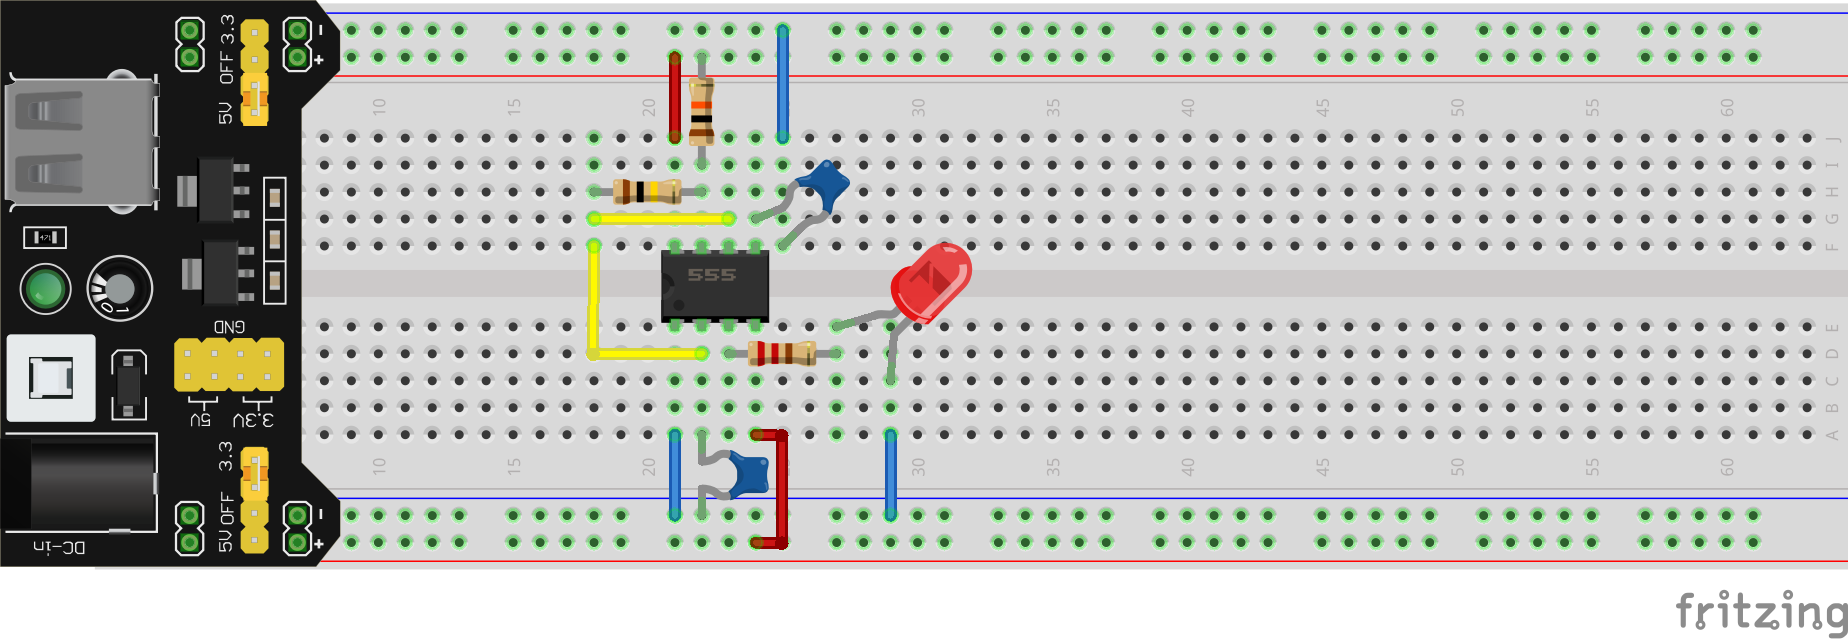
\includegraphics[width=0.8\textwidth]{lesson_circuits/L11/lesson_11.png}
    \caption{555 LED flasher Breadboard Schematic}
    \label{fig:555_led_sch}
\end{figure}
\begin{figure}[!htp]
    \centering
    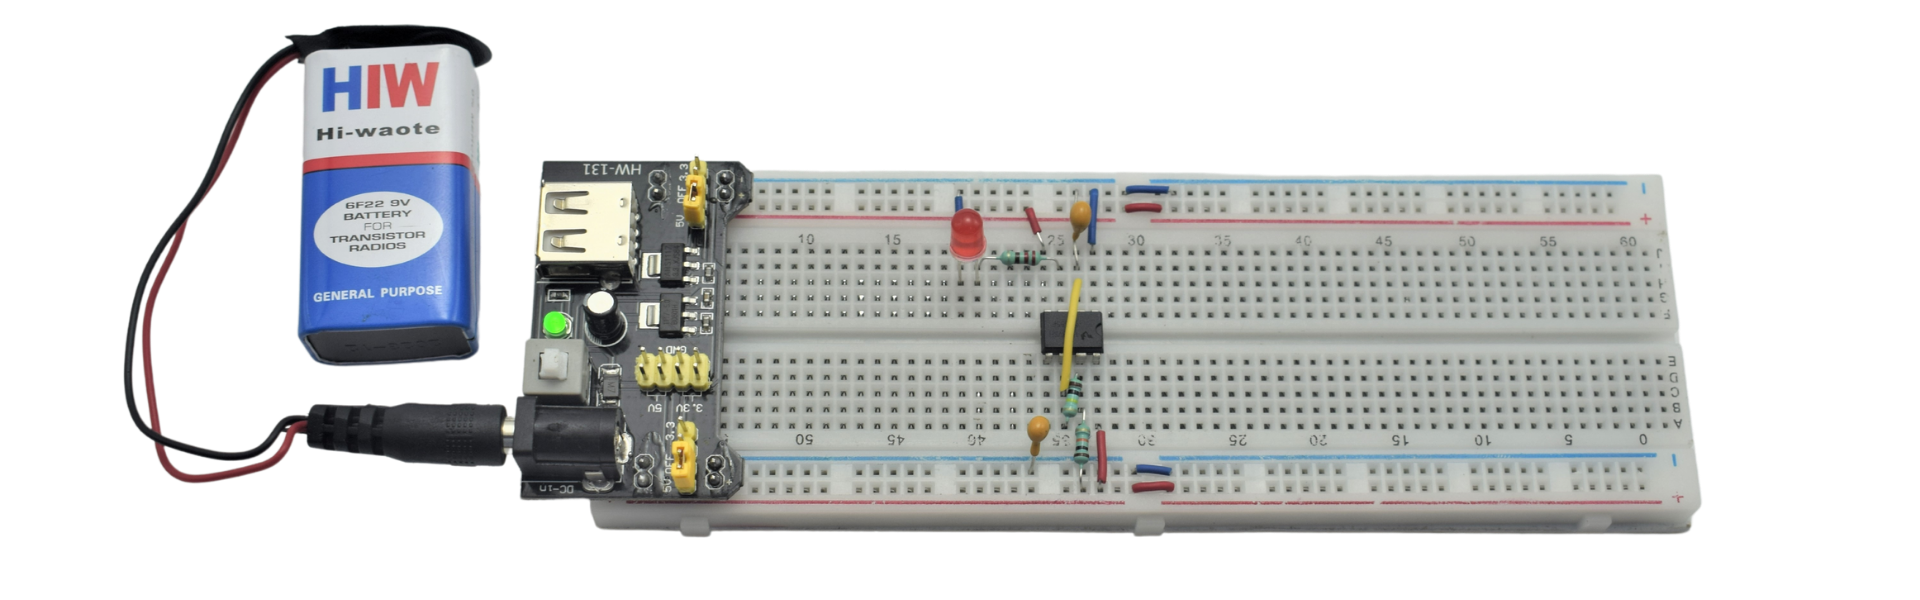
\includegraphics[width=\textwidth]{lesson_circuits/L11/L11-A.png}
    \caption{555 LED flasher: LED OFF}
    \label{fig:555_led_obb}
\end{figure}
\begin{figure}[!htp]
    \centering
    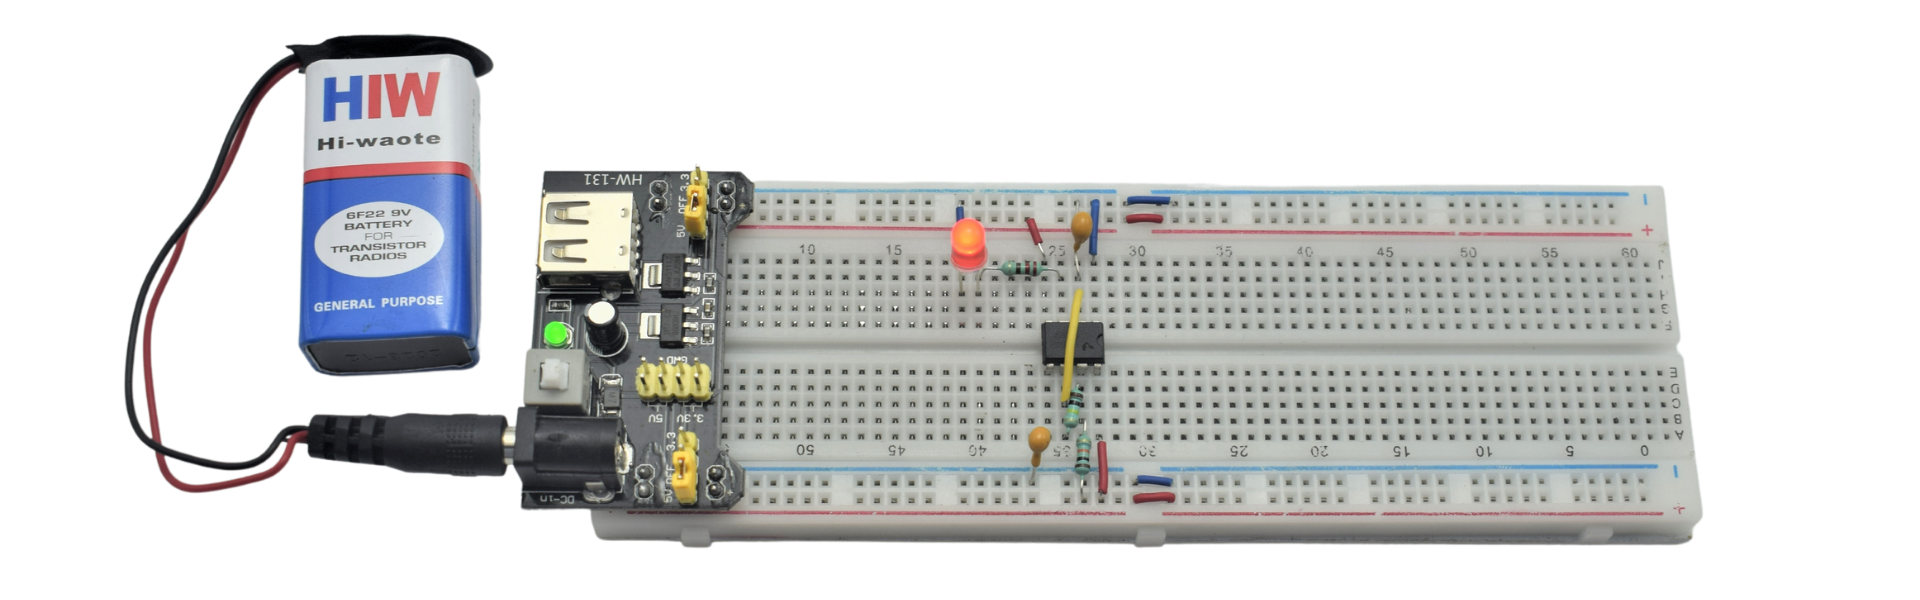
\includegraphics[width=\textwidth]{lesson_circuits/L11/L11-B.png}
    \caption{555 LED flasher: LED ON}
    \label{fig:555_led_obb1}
\end{figure}

\section{Lesson 12: 555 Dual LED Flasher}
\subsection{Objective}
In this activity we'll flash two LEDs on and off using astable 555 multivibrator circuit.
\subsection{Components Required}
\begin{enumerate}
    \item Breadboard Power Supply $\times$ 1
    \item 9V Battery $\times$ 1
    \item 9V Battery Connector $\times$ 1
    \item Breadboard $\times$ 1
    \item 555 IC $\times$ 1
    \item Red LED $\times$ 1
    \item Blue LED $\times$ 1
    \item \SI{220}{\ohm} $\times$ 2
    \item \SI{10}{\kilo\ohm} $\times$ 1
    \item \SI{100}{\kilo\ohm} $\times$ 1
    \item \SI{100}{\nano\farad} $\times$ 1
    \item \SI{10}{\micro\farad} $\times$ 1
    \item Male-Male jumper wire $\times$ 7
\end{enumerate}
\subsection{Circuit}
\begin{figure}[!htp]
    \centering
    \begin{circuitikz}[scale = 1.2]
        \TIMER555(0,0){1}
        \draw (1 GND) to[short, -*] ++(0,-0.7) node[ground](g1){};
        \draw (1 CTRL) to[C, l=$100\si{\nano\farad}$] ++(0,-0.5)
            to[short, -*] ++(0,-0.2)node[](ctr){} |- (g1);
        \draw (1 VCC) to[short, -*] ++(0,0.5) node[vcc](v1){$V_{cc}$};
        \draw (1 RESET) |- (v1);
        \draw (1 THR) to[short, -*] ++(-0.5,0) node[](s6){};
        \draw (1 TRG) to[short, -*] ++(-0.5,0) node[](s2){};
        \draw (1 DIS) to[short, -*] ++(-0.5,0) node[](s7){};
        \draw (s7) to[R, l_=$10\si{\kohm}$] ($(1 THR)-(0.5,0)$);
        \draw (s7) to[R, l=$100\si{\kohm}$] ++(0,1.5) |- (v1);
        \draw (s6) -- (s2) to[C, l_=$10\si{\micro\farad}$] ++(0,-1.5) |- (g1);
        \draw (1 OUT) to[short, -*] ++(0.5,0)node[](ll){} -- ++(0,-0.5) 
            to[R, l=$220\si{\ohm}$] ++ (0,-1)
            to[empty led, color=red] ++(0,-1.5) |- (ctr);
        \draw (ll) -- ++(0,0.5) 
            to[R, l=$220\si{\ohm}$] ++ (0,1)
            to[empty led, color=blue, invert, mirror] ++(0,1.5)
            to[short,-*] ++(-1.6,0);
    \end{circuitikz}
    \caption{555 Dual LED Flasher Circuit}
    \label{fig:555_dual_led_cir}
\end{figure}
\subsection{Circuit Explanation}
The circuit operates in astable mode as explained in section \ref{astablemode}. In this circuit one more LED is connected between 
the output pin and $V_{cc}$, in such a way that it glows up when output is low and turns off when output is high.
\subsection{Circuit Picture}
\begin{figure}[!htp]
    \centering
    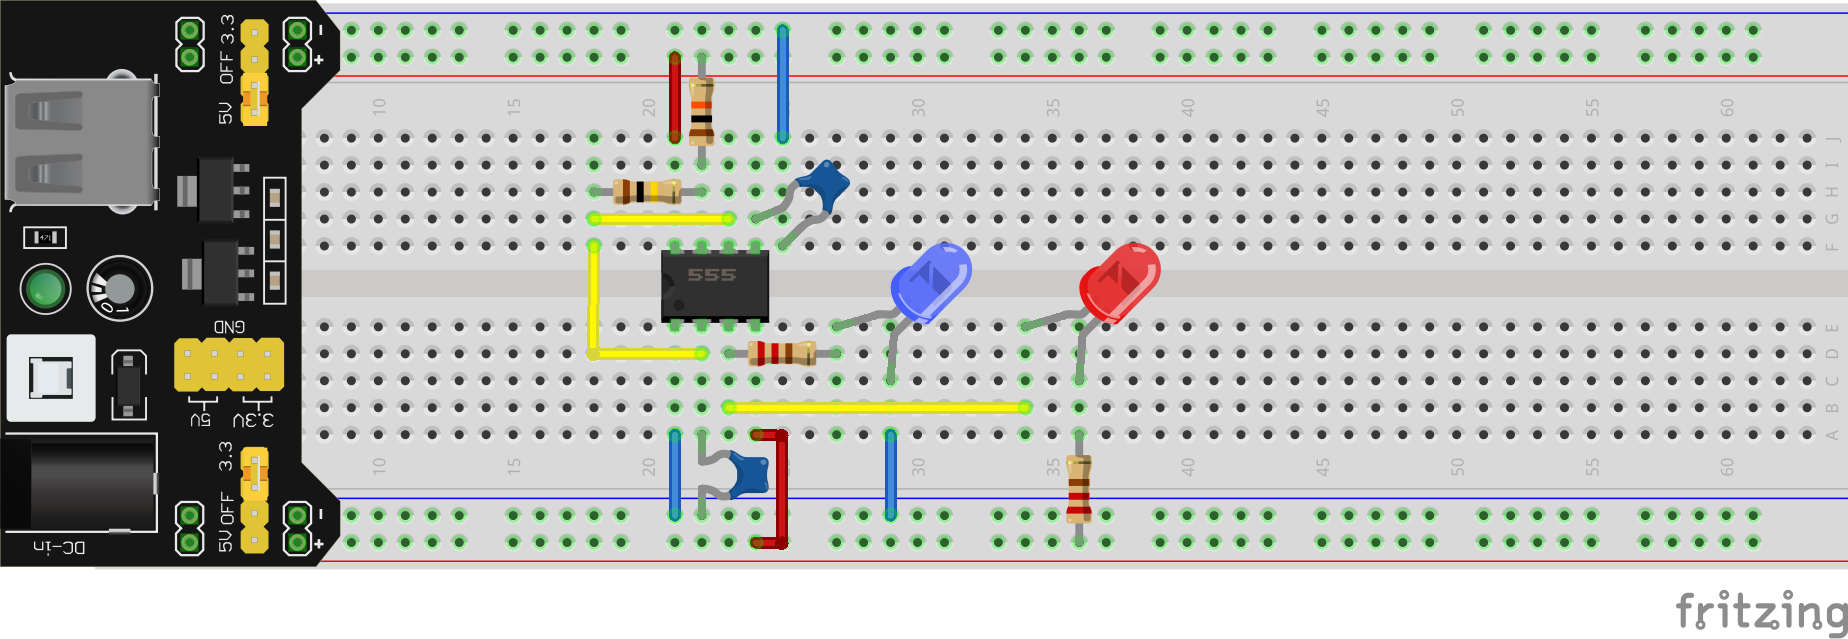
\includegraphics[width=0.8\textwidth]{lesson_circuits/L12/lesson_12.png}
    \caption{555 Dual LED flasher Breadboard Schematic}
    \label{fig:555_2led_sch}
\end{figure}
\begin{figure}[!htp]
    \centering
    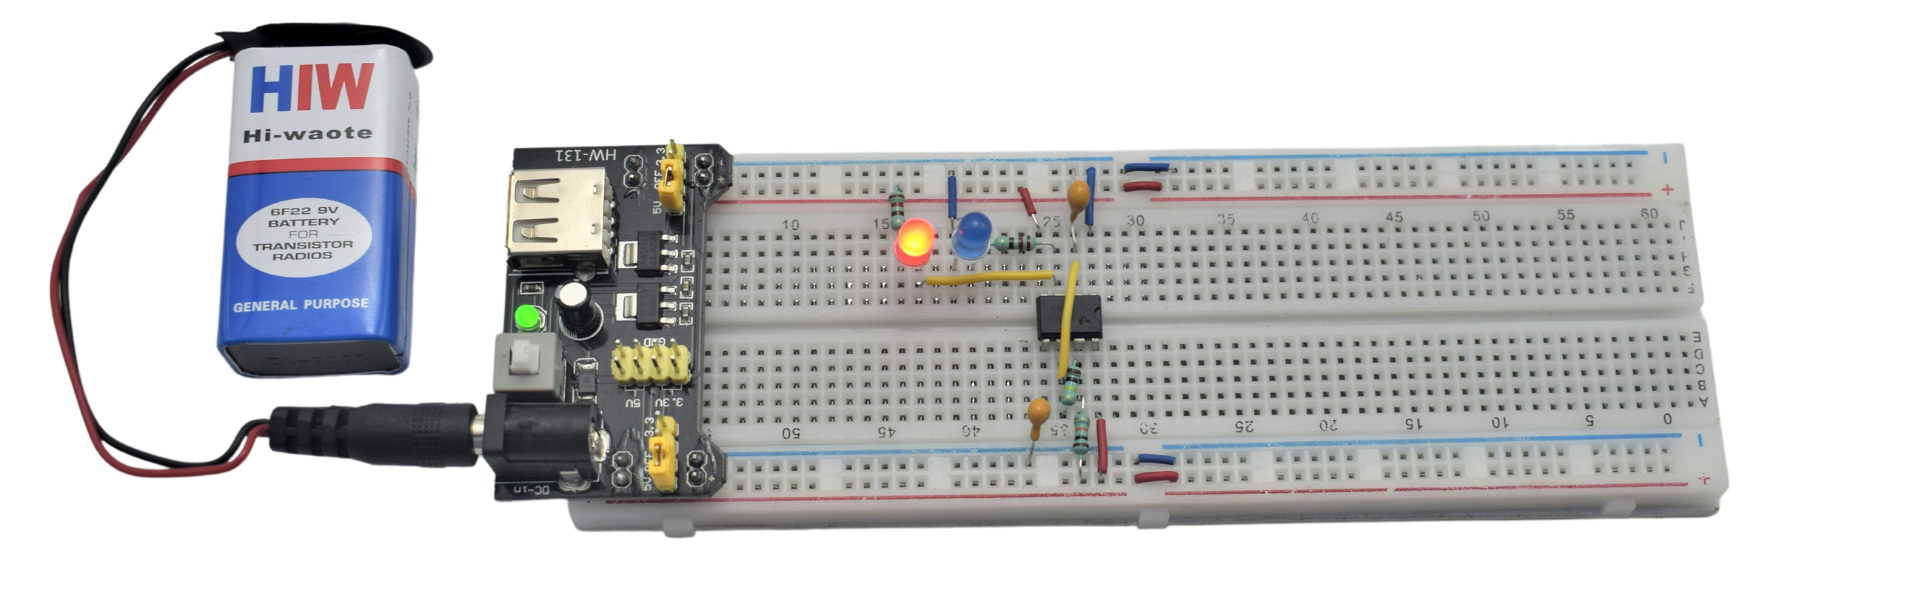
\includegraphics[width=\textwidth]{lesson_circuits/L12/L12-A.png}
    \caption{555 Dual LED flasher 1}
    \label{fig:555_2led_obb}
\end{figure}
\begin{figure}[!htp]
    \centering
    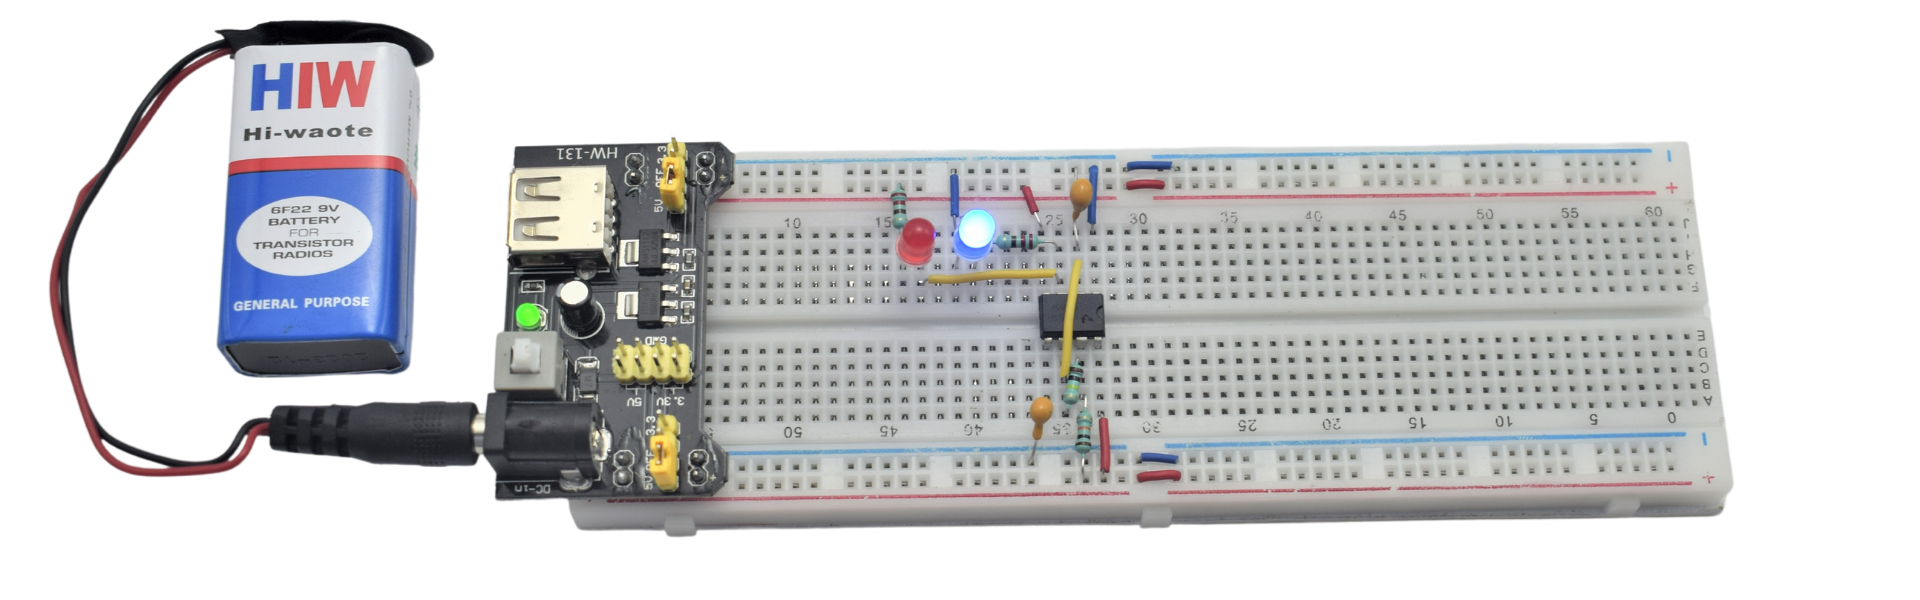
\includegraphics[width=\textwidth]{lesson_circuits/L12/L12-B.png}
    \caption{555 LED flasher 2}
    \label{fig:555_2led_obb1}
\end{figure}

\section{Lesson 13: Fading LED using 555}
\subsection{Objective}
In this activity we'll fade an LED up and down using astable 555 multivibrator circuit.
\subsection{Components Required}
\begin{enumerate}
    \item Breadboard Power Supply $\times$ 1
    \item 9V Battery $\times$ 1
    \item 9V Battery Connector $\times$ 1
    \item Breadboard $\times$ 1
    \item 555 IC $\times$ 1
    \item Red LED $\times$ 1
    \item 2N2222 $\times$ 1
    \item \SI{220}{\ohm} $\times$ 1
    \item \SI{10}{\kilo\ohm} $\times$ 1
    \item \SI{100}{\kilo\ohm} $\times$ 1
    \item \SI{1}{\Mohm} $\times$ 1
    \item \SI{100}{\nano\farad} $\times$ 1
    \item \SI{10}{\micro\farad} $\times$ 2
    \item Male-Male jumper wire $\times$ 11
\end{enumerate}
\subsection{Circuit}
\begin{figure}[!htp]
    \centering
    \begin{circuitikz}[scale = 1.2]
        \TIMER555(0,0){1}
        \draw (1 GND) to[short, -*] ++(0,-0.7) node[ground](g1){};
        \draw (1 CTRL) to[C, l=$100\si{\nano\farad}$] ++(0,-0.5)
            to[short, -*] ++(0,-0.2)node[](ctr){} |- (g1);
        \draw (1 VCC) to[short, -*] ++(0,0.5) node[vcc](v1){$V_{cc}$};
        \draw (1 RESET) to[short, -*] ++(0,0.5)node[](rst){} |- (v1);
        \draw (1 THR) to[short, -*] ++(-0.5,0) node[](s6){};
        \draw (1 TRG) to[short, -*] ++(-0.5,0) node[](s2){};
        \draw (1 DIS) to[short, -*] ++(-0.5,0) node[](s7){};
        \draw (s7) to[R, l_=$10\si{\kohm}$] ($(1 THR)-(0.5,0)$);
        \draw (s7) to[R, l=$100\si{\kohm}$] ++(0,1.5) |- (v1);
        \draw (s6) -- (s2) to[C, l_=$10\si{\micro\farad}$] 
            ++(0,-1.5) |- (g1);
        \draw ($(1 OUT) + (2,0)$) node[npn](t1){};
        \draw (1 OUT) to[R,l=$1\si{\Mohm}$] (t1.B);
        \draw (t1.B) to[short, *-] ++(0,-1)
                to[C, l_=$10\si{\uF}$] ++(0,-1.5)
                to[short, -*] ++(0,-0.7)node[](tt){} |- (ctr);
        \draw (t1.E) |- (tt);
        \draw (rst) to[R, l=$220\si{\ohm}$] ++(3.1,0)
                to[empty led, color=red] (t1.C);
    \end{circuitikz}
    \caption{Fading LED using 555}
    \label{fig:555_fade_led_cir}
\end{figure}
\subsection{Circuit Explanation}
In this circuit 555 operates in astable mode \ref{astablemode}. When the output is high, the capacitor connected to transistor base 
starts charging up, slowly lighting up the LED. And, as the output turns low, the capacitor slowly discharges through the transistor 
fading the LED off.
\subsection{Circuit Picture}
\begin{figure}[!htp]
    \centering
    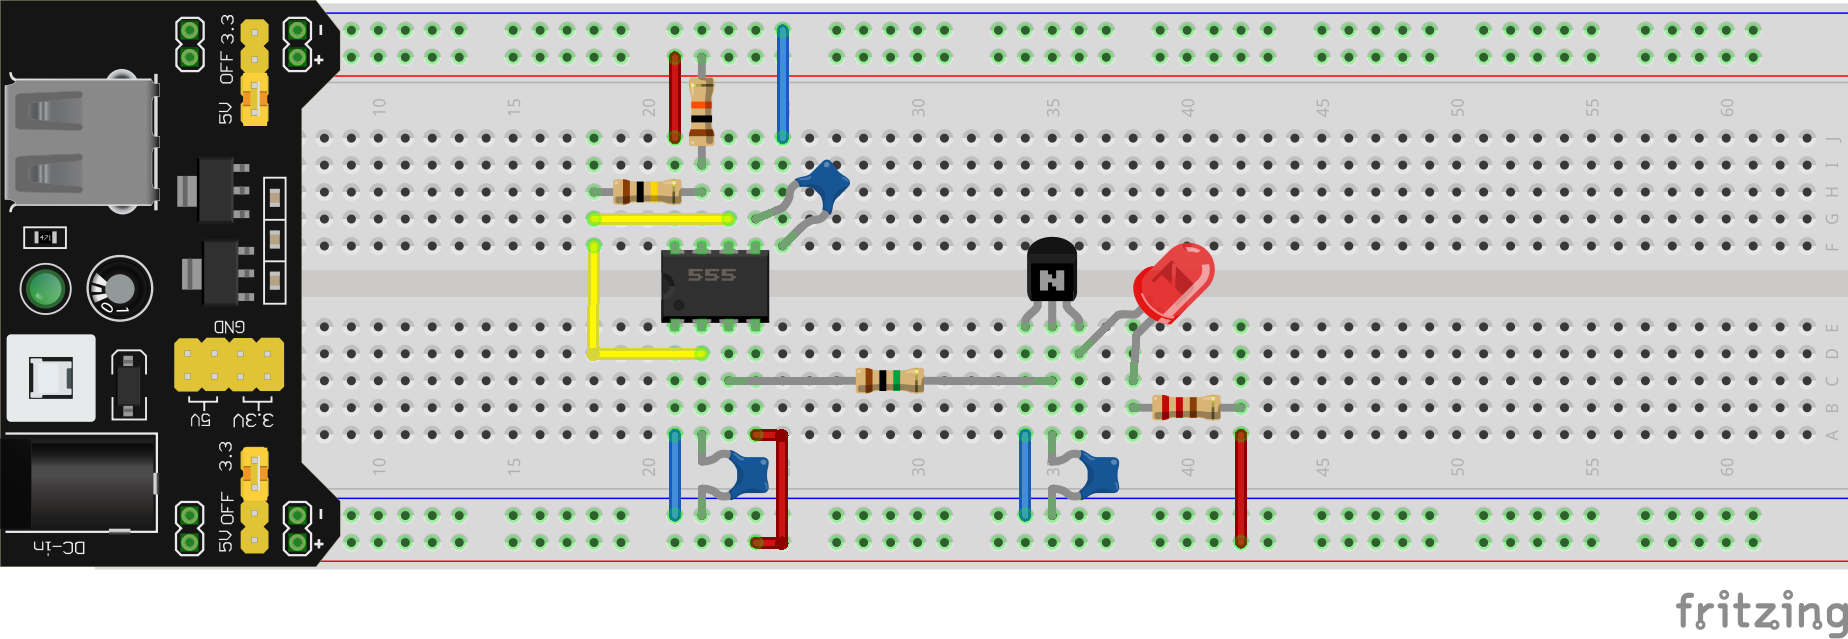
\includegraphics[width=0.8\textwidth]{lesson_circuits/L13/lesson_13.png}
    \caption{Fading LED using 555 Breadboard Schematic}
    \label{fig:555_fled_sch}
\end{figure}
\begin{figure}[!htp]
    \centering
    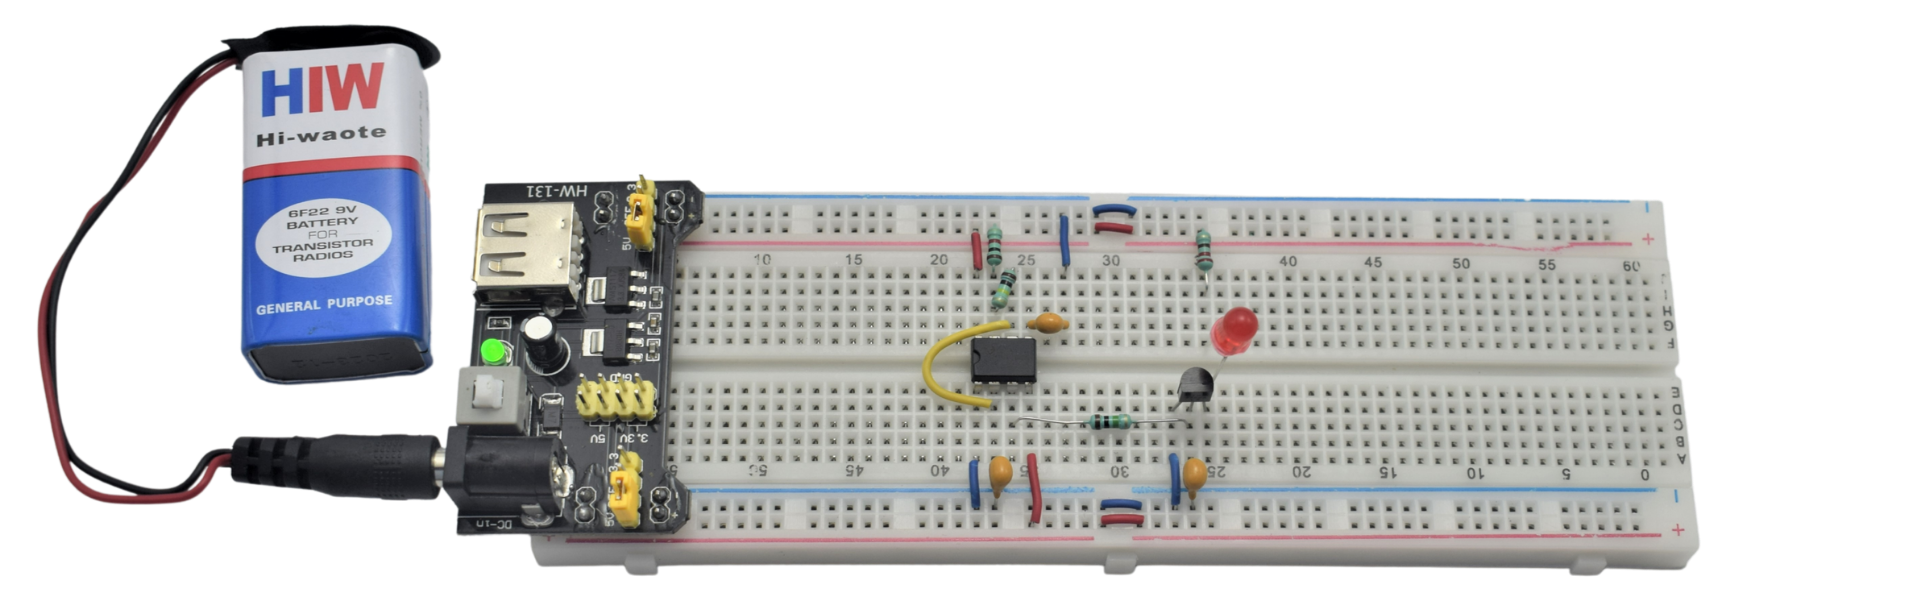
\includegraphics[width=\textwidth]{lesson_circuits/L13/L13-A.png}
    \caption{LED fading 1}
    \label{fig:555_fled_obb}
\end{figure}
\begin{figure}[!htp]
    \centering
    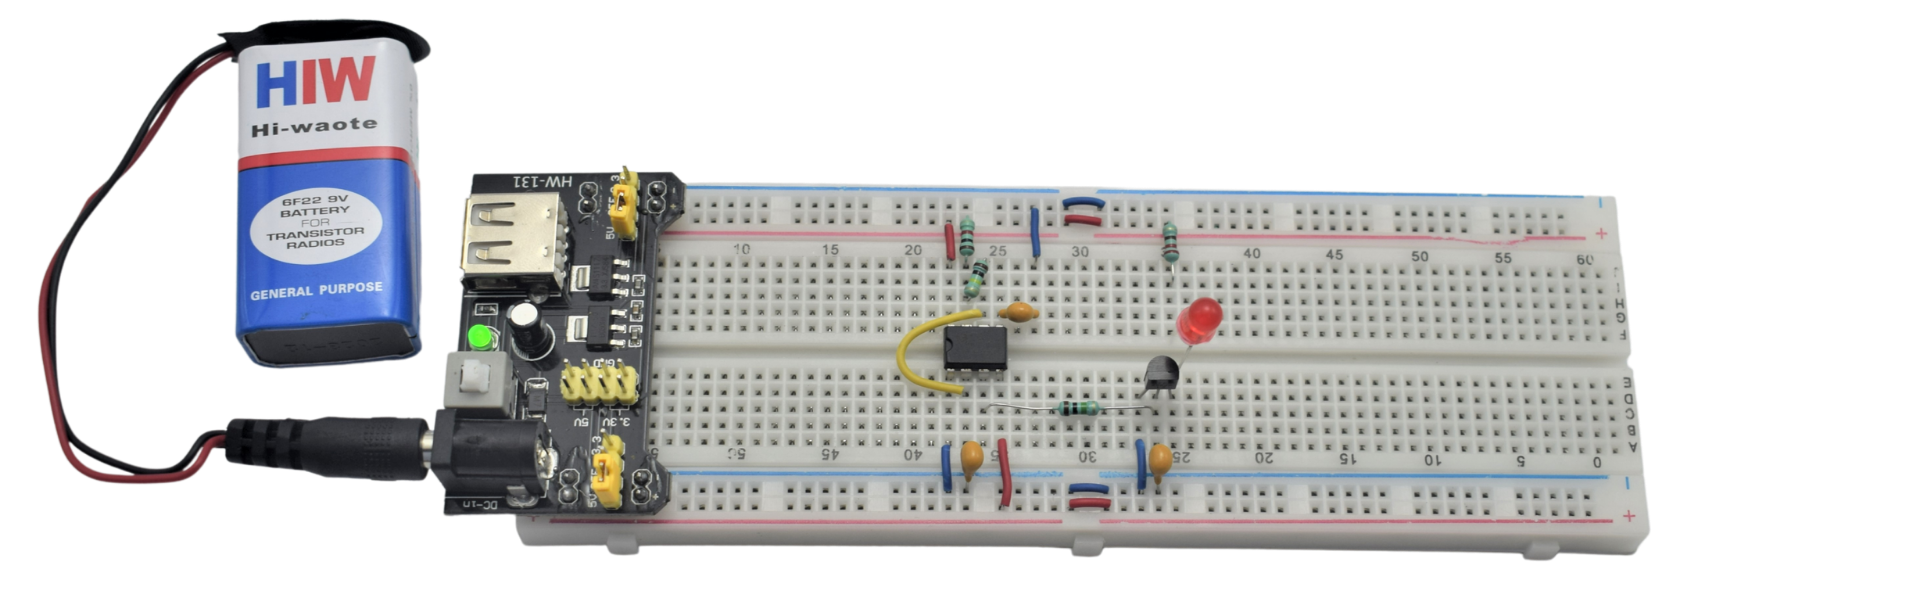
\includegraphics[width=\textwidth]{lesson_circuits/L13/L13-B.png}
    \caption{LED fading 2}
    \label{fig:555_fled_obb1}
\end{figure}

\section{Lesson 14: Bistable Button Flip/Flop using 555}
\subsection{Objective}
In this activity we'll create bistable 555 circuit.
\subsection{Components Required}
\begin{enumerate}
    \item Breadboard Power Supply $\times$ 1
    \item 9V Battery $\times$ 1
    \item 9V Battery Connector $\times$ 1
    \item Breadboard $\times$ 1
    \item 555 IC $\times$ 1
    \item Red LED $\times$ 1
    \item Push Button $\times$ 2
    \item \SI{220}{\ohm} $\times$ 1
    \item \SI{10}{\kilo\ohm} $\times$ 2
    \item \SI{100}{\nano\farad} $\times$ 2
    \item Male-Male jumper wire $\times$ 9
\end{enumerate}
\subsection{Circuit}
\begin{figure}[!htp]
    \centering
    \begin{circuitikz}[scale = 1.2]
        \TIMER555(0,0){1}
        \draw (1 GND) to[short, -*] ++(0,-0.7) node[ground](g1){};
        \draw (1 CTRL) to[C, l=$100\si{\nano\farad}$] ++(0,-0.5)
            to[short, -*] ++(0,-0.2)node[](ctr){} |- (g1);
        \draw (1 VCC) to[short, -*] ++(0,0.5) node[vcc](v1){$V_{cc}$};
        \draw (1 RESET) -- ++(0,0.2) -- ++(-3.5,0) -- ++(0,-3)
            to[short, -*] ++(-0.5,0)node[](br){} to[R,l=$10\si{\kohm}$] 
            ++(0,3.3)node[](j1){} |- (v1);
        \draw (1 TRG) to[short, -*] ++(-2,0)node[](bt){} 
            -- ++(0,1.2) to[R, l=$10\si{\kohm}$] ++(0,3.3) 
            to[short, -*] (j1);
        \draw (bt) to[push button, mirror, l_=TRIG] ++(0,-1.5) |- (g1);
        \draw (br) -- ++(0,-1.2) to[push button, l=RST] ++(0,-1.5) |- (g1);
        \draw (1 OUT) -- ++(0.5,0) -- ++(0,-0.5) 
            to[R, l=$220\si{\ohm}$] ++ (0,-1)
            to[empty led, color=red] ++(0,-1.5) |- (ctr);
    \end{circuitikz}
    \caption{Bistable Button Flip/Flop Circuit}
    \label{fig:555_bistable_cir}
\end{figure}
\subsection{Circuit Explanation}
This circuit is explained in section \ref{bistablemode}
\subsection{Circuit Picture}
\begin{figure}[!htp]
    \centering
    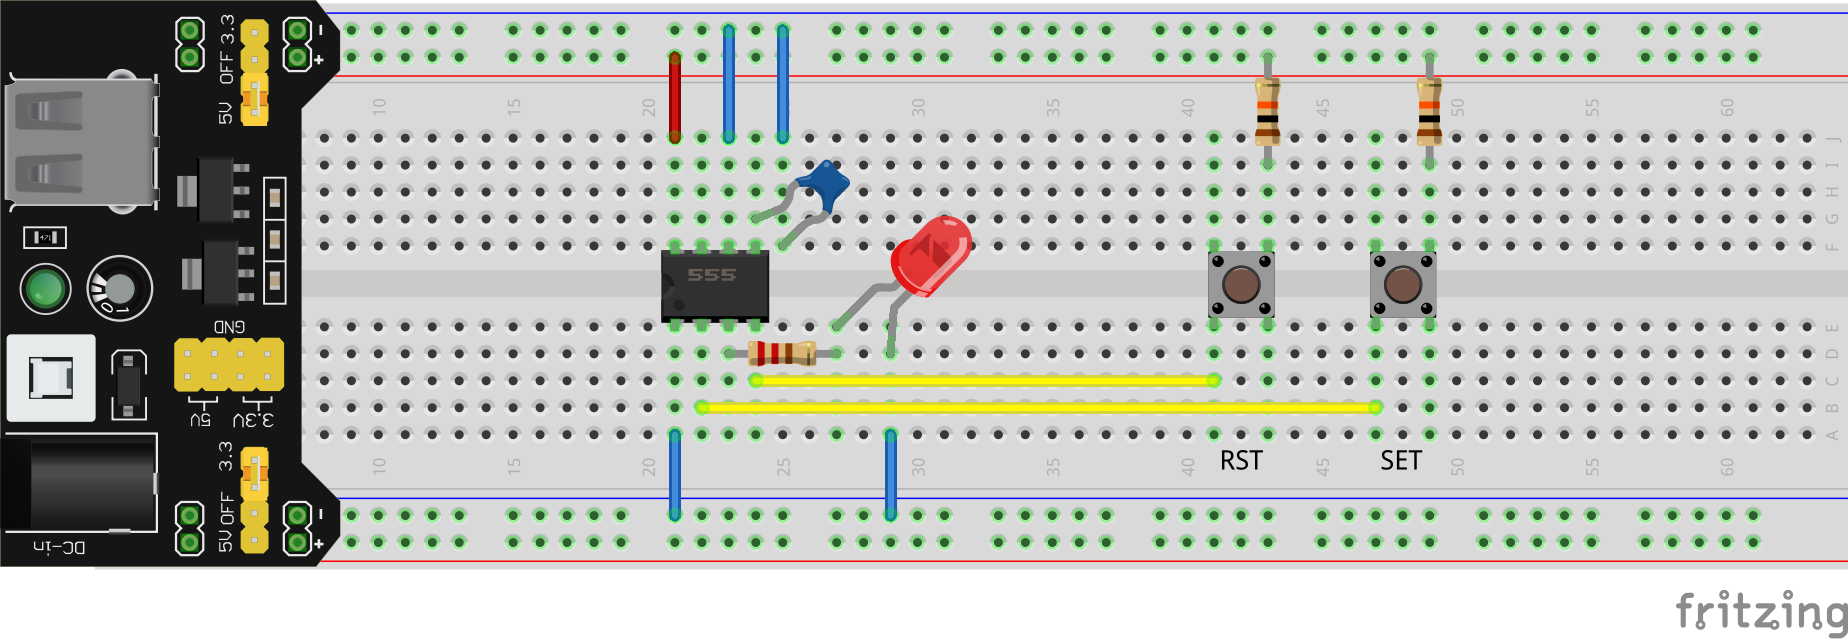
\includegraphics[width=0.8\textwidth]{lesson_circuits/L14/lesson_14.png}
    \caption{Bistable Button Flip/Flop using 555 Breadboard Schematic}
    \label{fig:555_ff_sch}
\end{figure}
\begin{figure}[!htp]
    \centering
    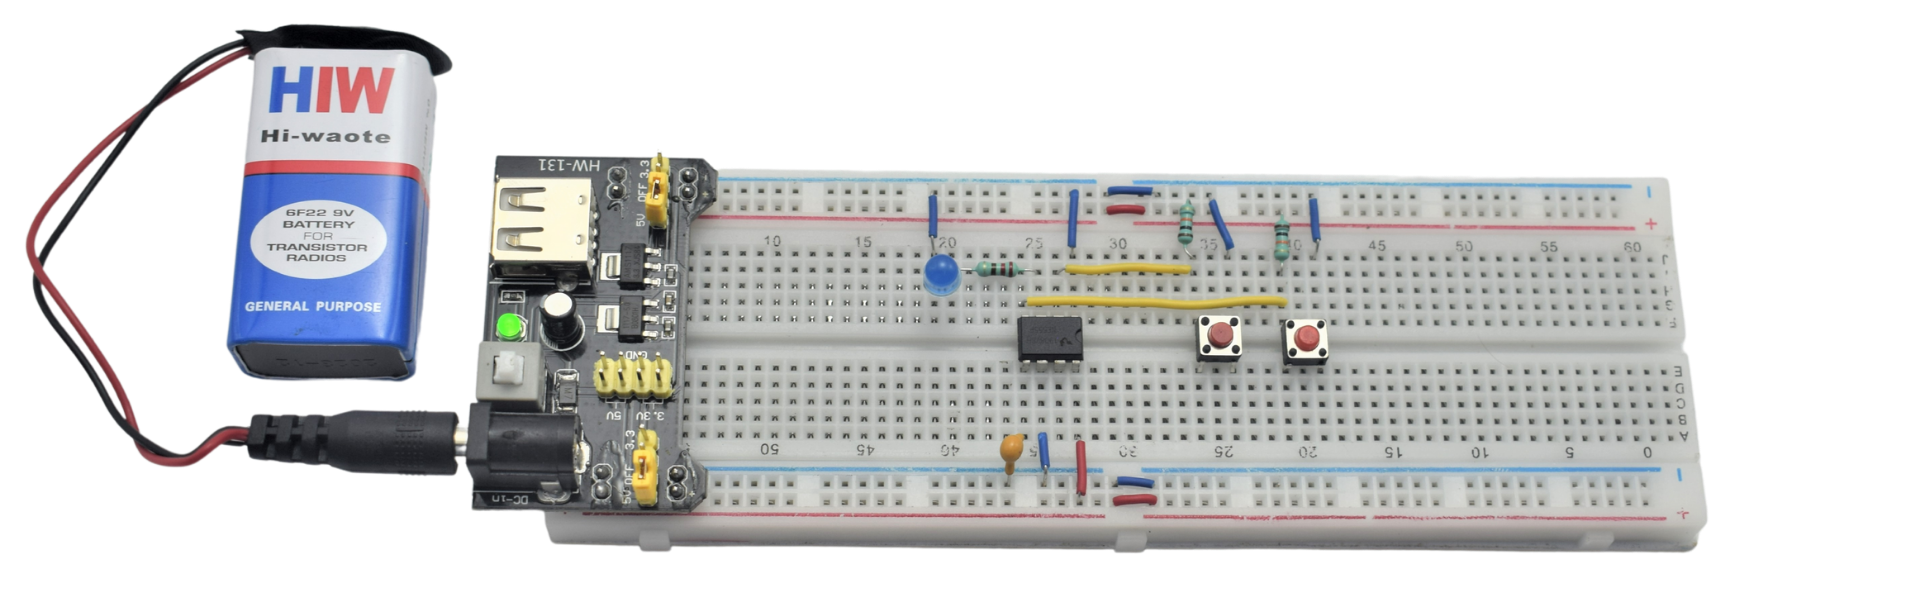
\includegraphics[width=\textwidth]{lesson_circuits/L14/L14-A.png}
    \caption{FF Idle}
    \label{fig:555_ff_obb}
\end{figure}
\begin{figure}[!htp]
    \centering
    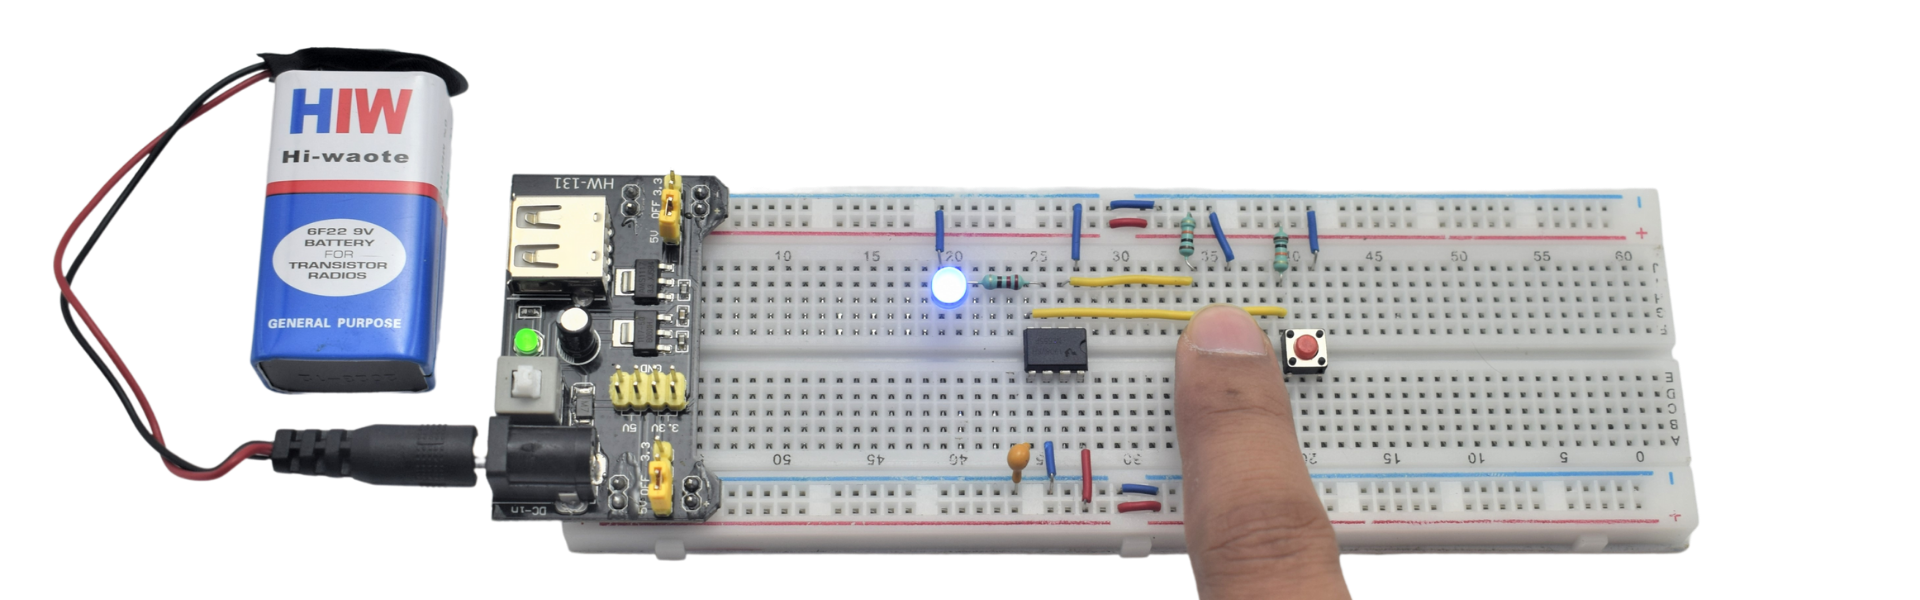
\includegraphics[width=\textwidth]{lesson_circuits/L14/L14-B.png}
    \caption{FF SET Button Pressed}
    \label{fig:555_ff_obb1}
\end{figure}
\begin{figure}[!htp]
    \centering
    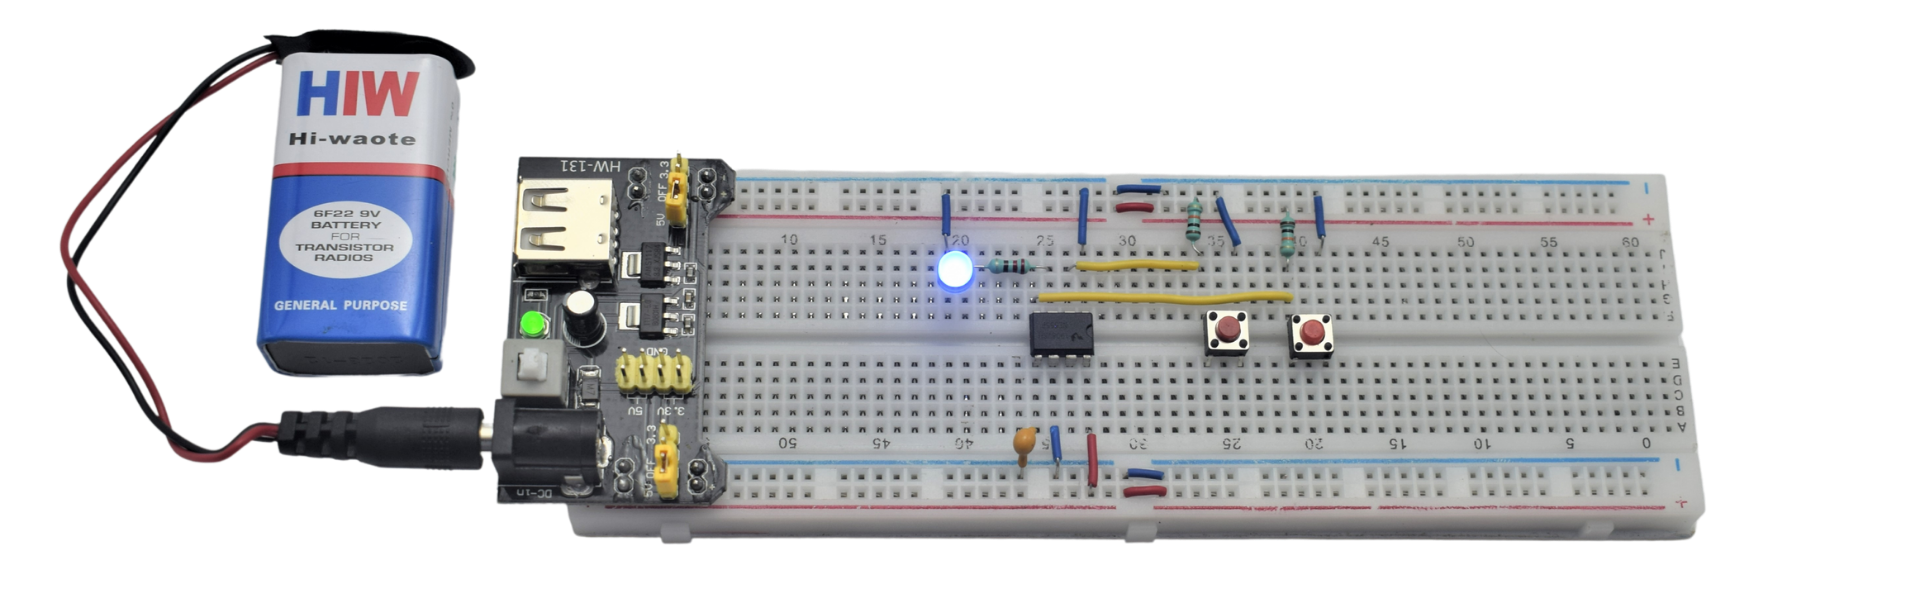
\includegraphics[width=\textwidth]{lesson_circuits/L14/L14-C.png}
    \caption{FF Idle after leaving SET button}
    \label{fig:555_ff_obb2}
\end{figure}
\begin{figure}[!htp]
    \centering
    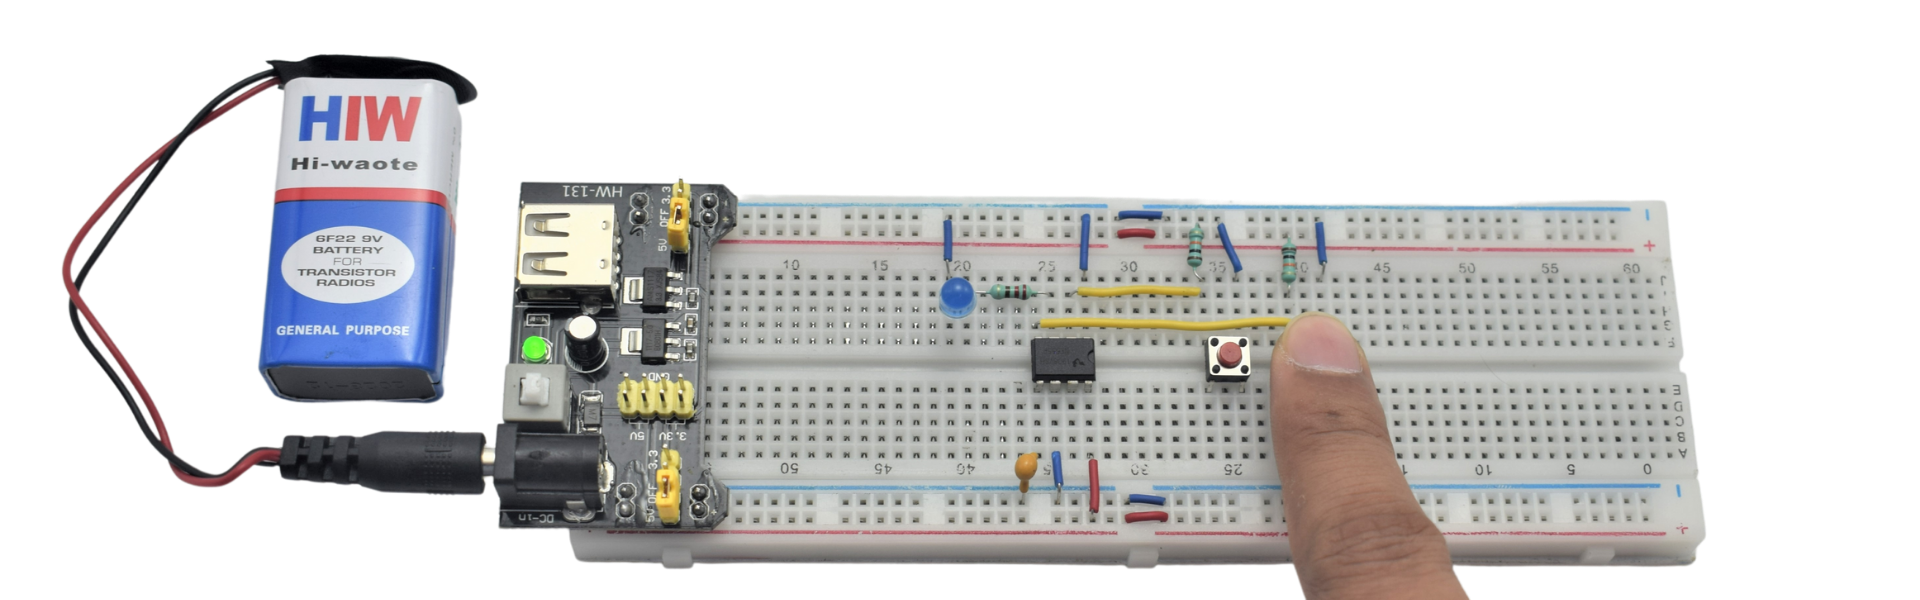
\includegraphics[width=\textwidth]{lesson_circuits/L14/L14-D.png}
    \caption{FF RST Button Pressed}
    \label{fig:555_ff_obb3}
\end{figure}
\begin{figure}[!htp]
    \centering
    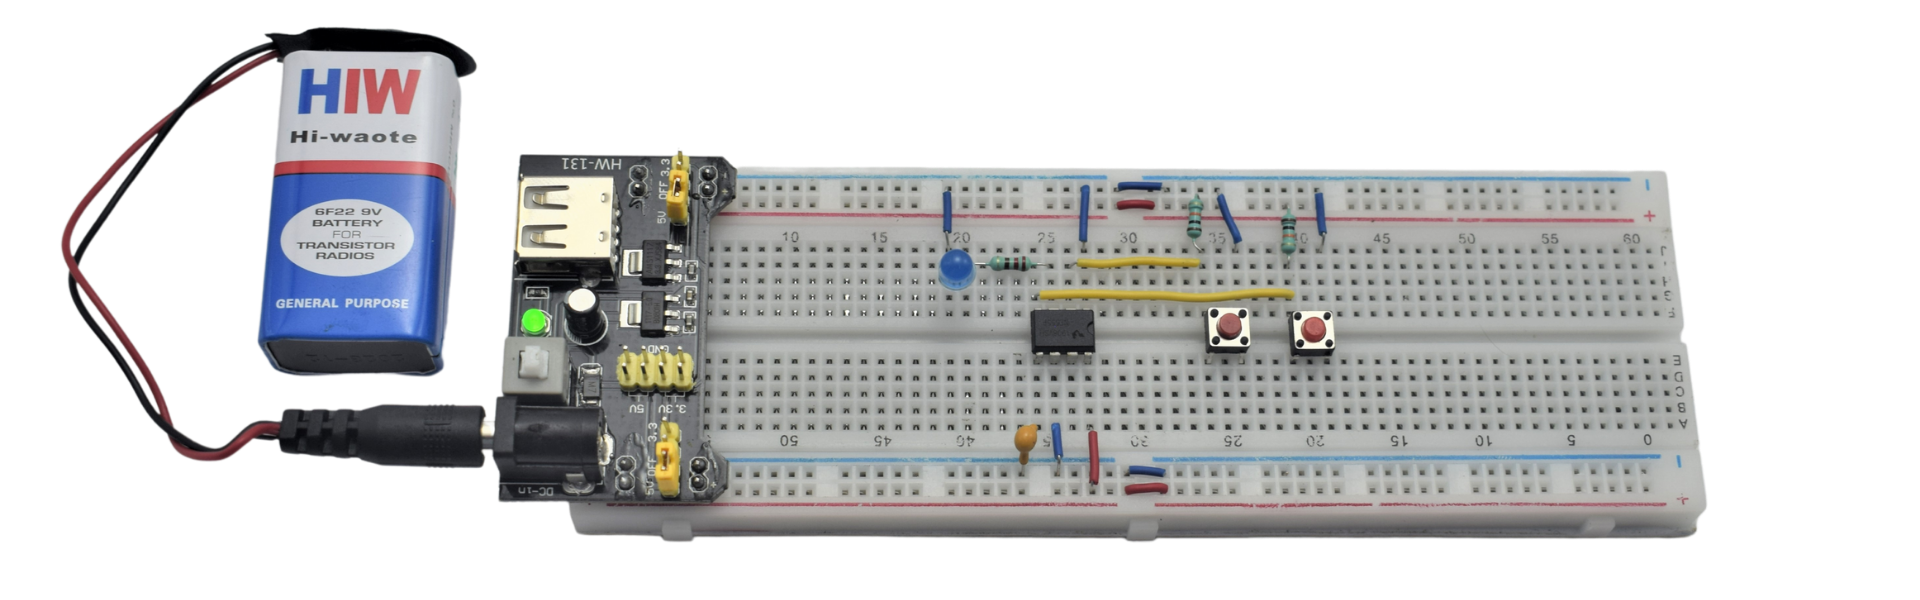
\includegraphics[width=\textwidth]{lesson_circuits/L14/L14-E.png}
    \caption{FF Idle after leaving RST Button}
    \label{fig:555_ff_obb4}
\end{figure}
\section{Lesson 15: Toggle Switch with 555}
\subsection{Objective}
In this activity we'll create a toggle switch using bistable 555 circuit.
\subsection{Components Required}
\begin{enumerate}
    \item Breadboard Power Supply $\times$ 1
    \item 9V Battery $\times$ 1
    \item 9V Battery Connector $\times$ 1
    \item Breadboard $\times$ 1
    \item 555 IC $\times$ 1
    \item Red LED $\times$ 1
    \item Push Button $\times$ 1
    \item \SI{220}{\ohm} $\times$ 1
    \item \SI{10}{\kilo\ohm} $\times$ 2
    \item \SI{100}{\kilo\ohm} $\times$ 1
    \item \SI{100}{\nano\farad} $\times$ 2
    \item Male-Male jumper wire $\times$ 11
\end{enumerate}
\subsection{Circuit}
\begin{figure}[!htp]
    \centering
    \begin{circuitikz}[scale = 1.2]
        \TIMER555(0,0){1}
        \draw (1 GND) to[short, -*] ++(0,-0.7) node[ground](g1){};
        \draw (1 CTRL) to[C, l=$100\si{\nano\farad}$] ++(0,-0.5)
            to[short, -*] ++(0,-0.2)node[](ctr){} |- (g1);
        \draw (1 VCC) to[short, -*] ++(0,0.5) node[vcc](v1){$V_{cc}$};
        \draw (1 RESET) |- (v1);
        \draw (1 THR) to[short, -*] ++(-0.5,0) node[](s6){};
        \draw (1 TRG) to[short, -*] ++(-0.5,0) node[](s2){};
        \draw (s6) -- (s2);
        \draw (s6) to[R, l=$10\si{\kohm}$] ++(0,3) |- (v1);
        \draw (s2) to[R, l=$10\si{\kohm}$] ++(0,-1.7) |- (g1);
        \draw (1 OUT) -- ++(0.5,0)node[circ](oo){} -- ++(0,-0.5) 
            to[R, l=$220\si{\ohm}$] ++ (0,-1)
            to[empty led, color=red] ++(0,-1.7)node[circ](g2){} |- (ctr);
        \draw (oo) to[R, l=$100\si{\kohm}$] ++(1.5,0)node[circ](rc){}
            to[C, l=$100\si{\nF}$] ++(0,-2) |- (g2);
        \draw (rc) to[push button, mirror] ++(0,2.5) -- ++(-8,0) |- (s6);
    \end{circuitikz}
    \caption{Toggle Switch with 555 Circuit}
    \label{fig:555_toggle_cir}
\end{figure}
\subsection{Circuit Explanation}
In this circuit we control the voltage at pin 2 and 6 of the 555 IC with help of the push button and capacitor. When the circuit is 
powered on the capacitor $C_2$ is discharged, therefore it's upper plate is close to 0 volts. When the switch is pressed the voltage 
at pin 2 goes low, turning the output of 555 on. Now the LED is on and the capacitor starts charging.

Now, if we again press the switch, the capacitor is charged, therefore the upper plate is close to $V_{out}$ which makes the voltage 
at pin 6 high, turning the 555 output low. Now the capacitor discharges through the 555 output pin and LED is turned off.
\subsection{Circuit Picture}
\begin{figure}[!htp]
    \centering
    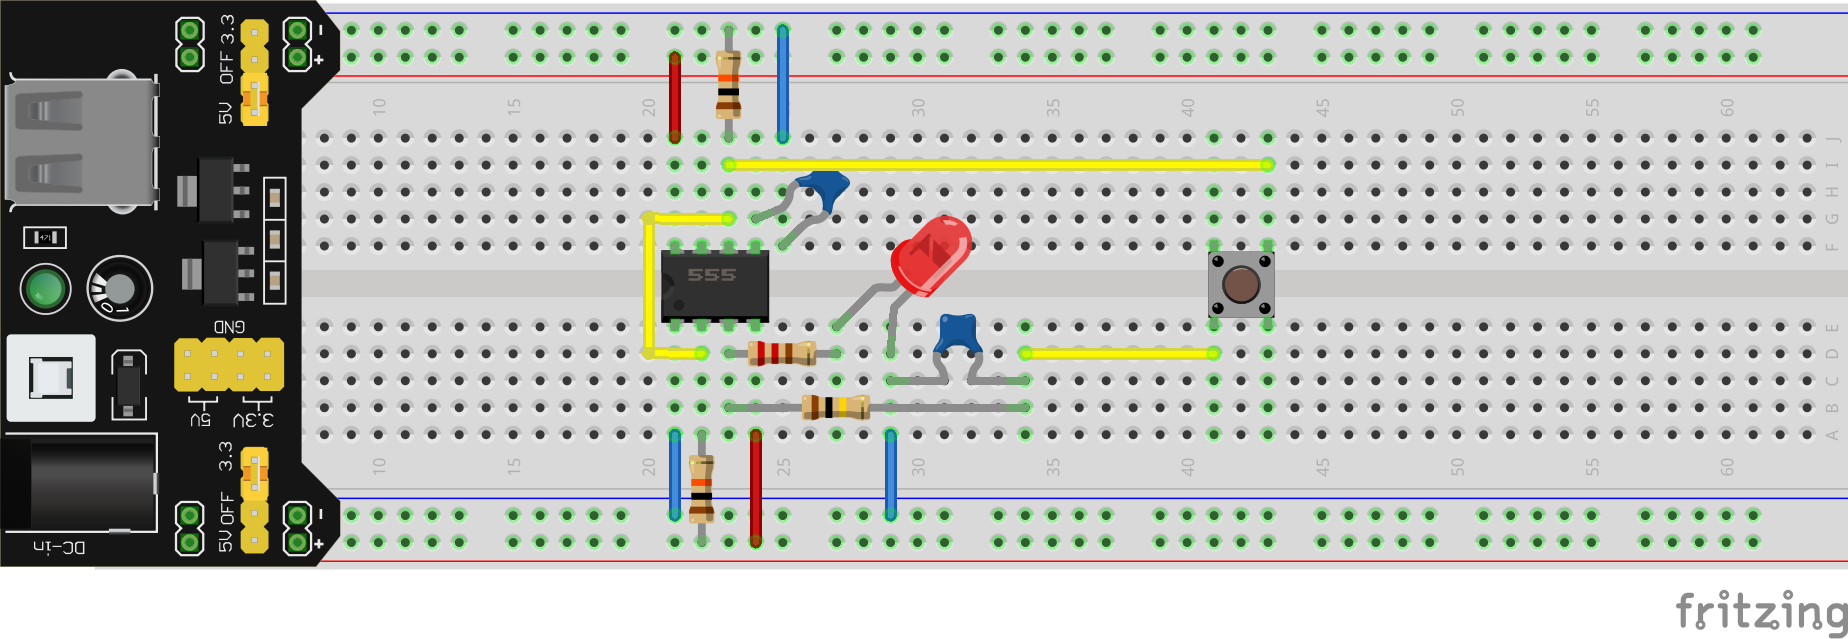
\includegraphics[width=0.8\textwidth]{lesson_circuits/L15/lesson_15.png}
    \caption{Toggle Switch using 555 Breadboard Schematic}
    \label{fig:555_ts_sch}
\end{figure}
\begin{figure}[!htp]
    \centering
    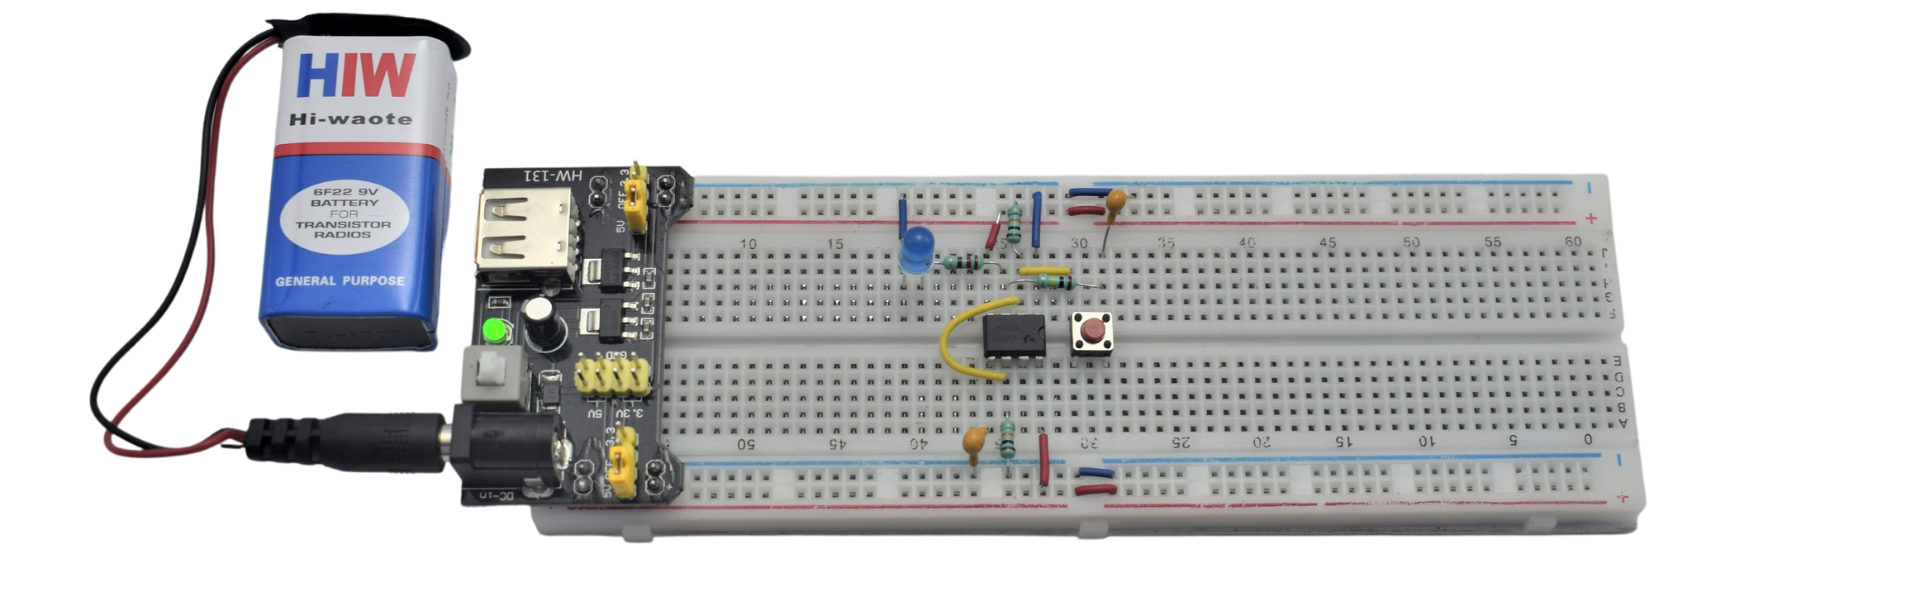
\includegraphics[width=\textwidth]{lesson_circuits/L15/L15-A.png}
    \caption{Idle}
    \label{fig:555_ts_obb}
\end{figure}
\begin{figure}[!htp]
    \centering
    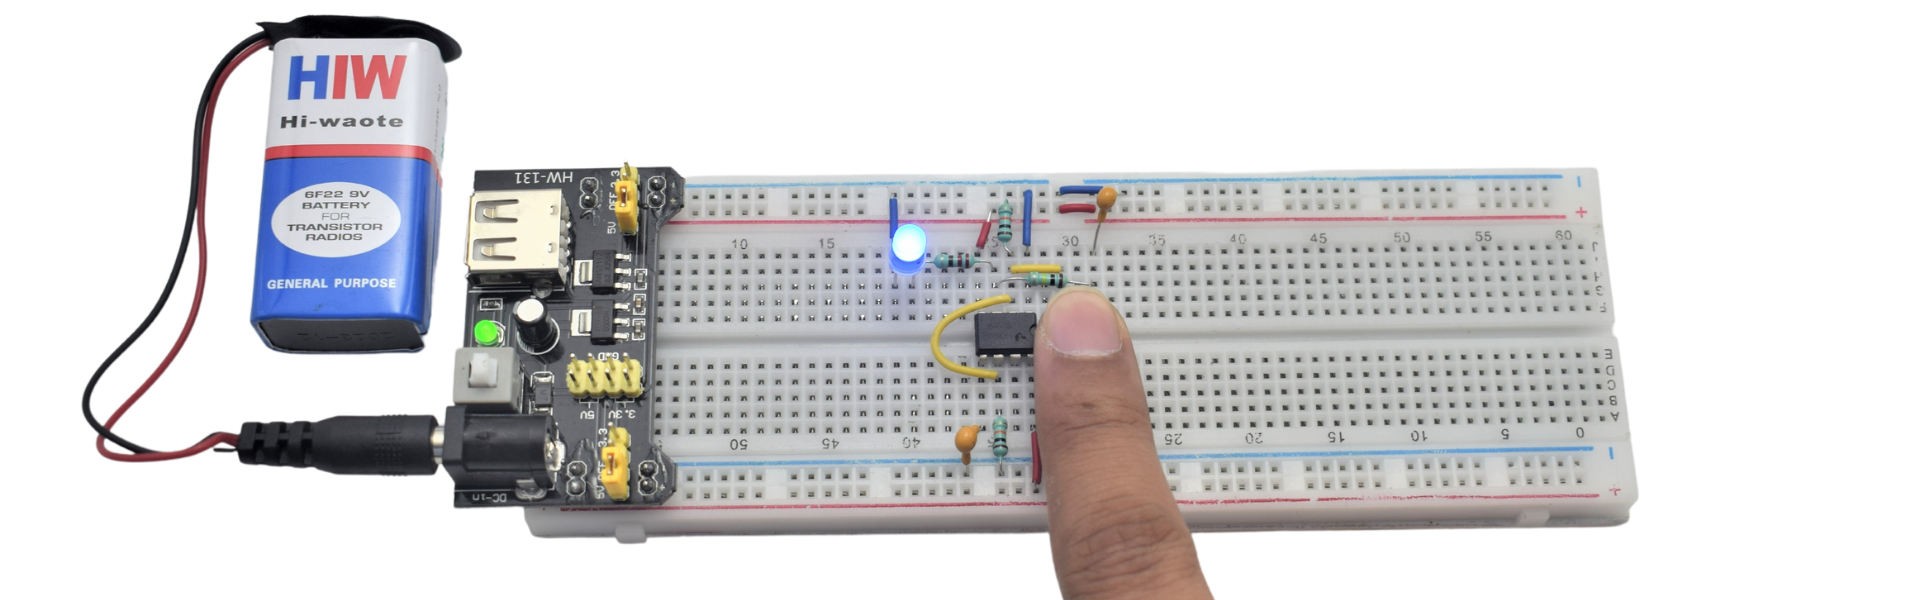
\includegraphics[width=\textwidth]{lesson_circuits/L15/L15-B.png}
    \caption{Button Pressed: LED turned ON}
    \label{fig:555_ts_obb1}
\end{figure}
\begin{figure}[!htp]
    \centering
    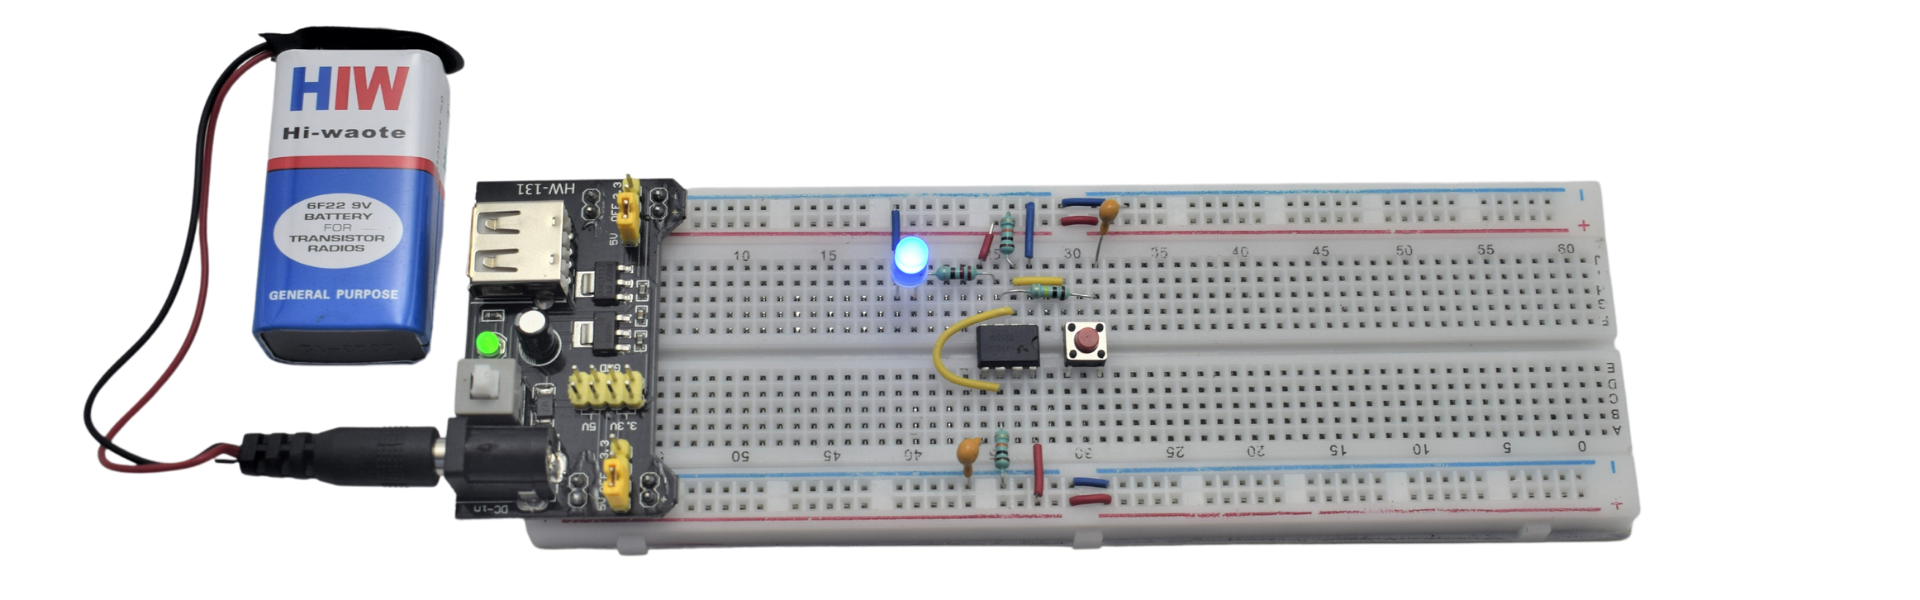
\includegraphics[width=\textwidth]{lesson_circuits/L15/L15-C.png}
    \caption{Button released}
    \label{fig:555_ts_obb2}
\end{figure}
\begin{figure}[!htp]
    \centering
    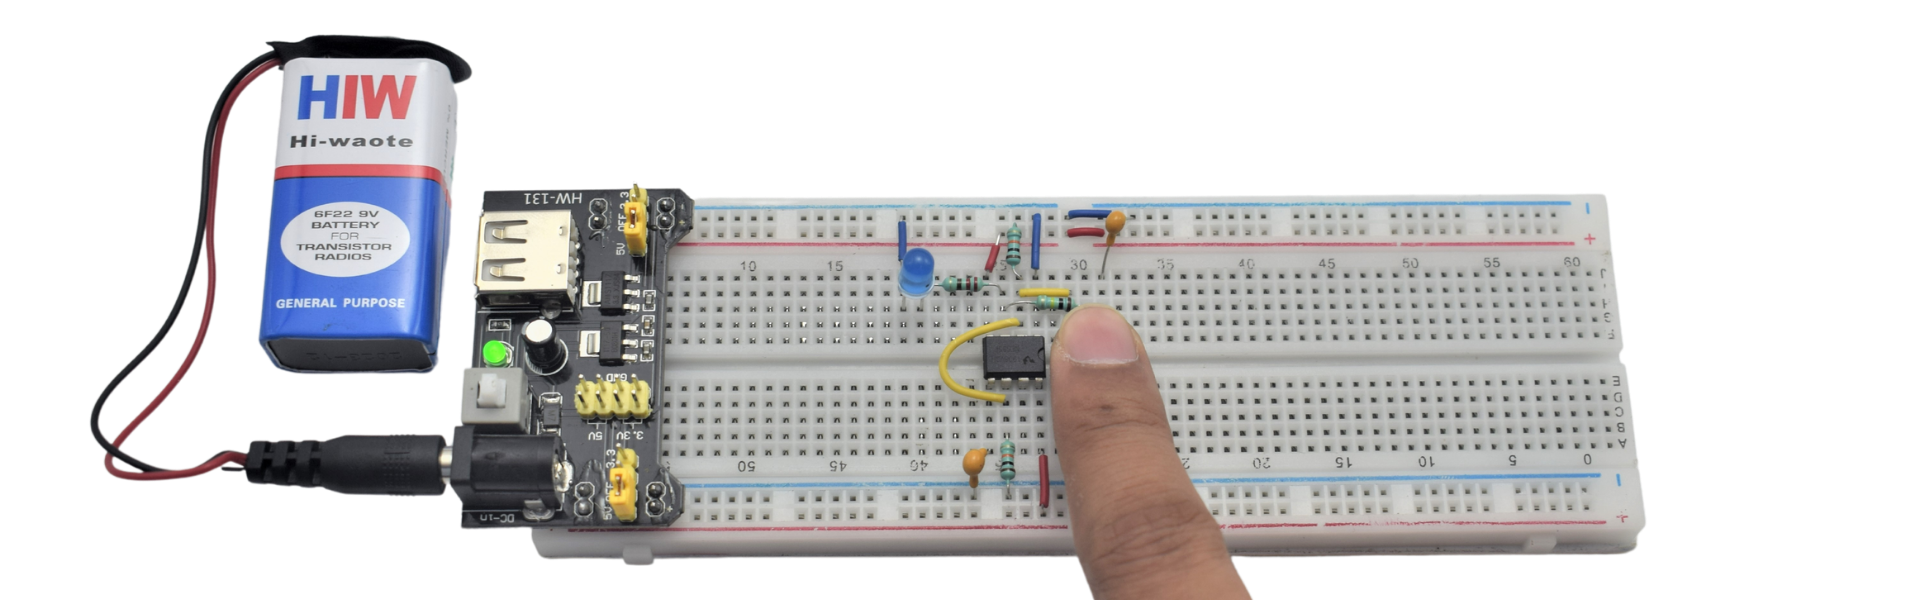
\includegraphics[width=\textwidth]{lesson_circuits/L15/L15-D.png}
    \caption{Button Pressed: LED turned OFF}
    \label{fig:555_ts_obb3}
\end{figure}
\begin{figure}[!htp]
    \centering
    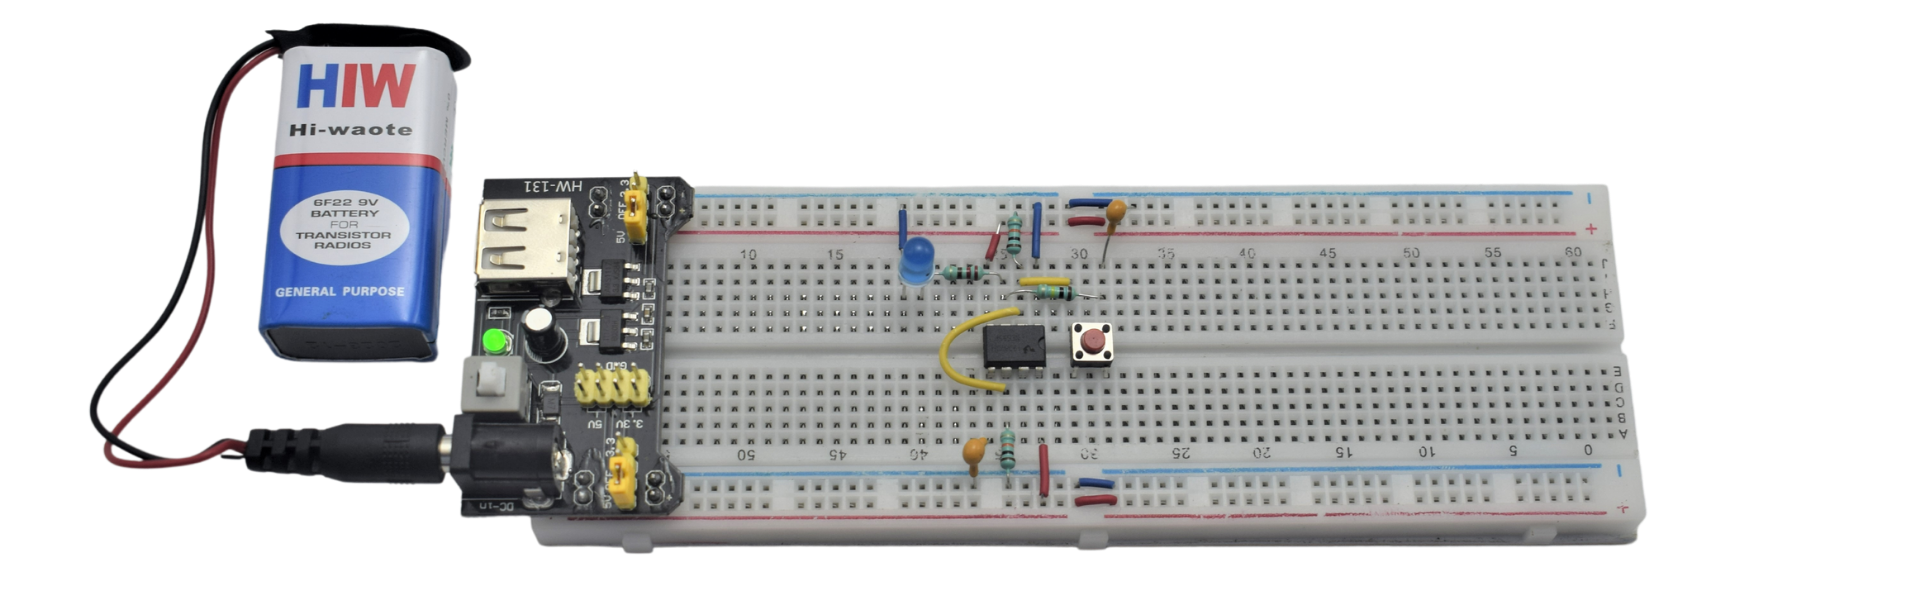
\includegraphics[width=\textwidth]{lesson_circuits/L15/L15-E.png}
    \caption{Button released}
    \label{fig:555_ts_obb4}
\end{figure}
\section{Lesson 16: Timer Delay using 555}
\subsection{Objective}
In this activity we'll use monostable 555 circuit to turn on an LED for fixed duration.
\subsection{Components Required}
\begin{enumerate}
    \item Breadboard Power Supply $\times$ 1
    \item 9V Battery $\times$ 1
    \item 9V Battery Connector $\times$ 1
    \item Breadboard $\times$ 1
    \item 555 IC $\times$ 1
    \item Red LED $\times$ 1
    \item Push Button $\times$ 1
    \item \SI{220}{\ohm} $\times$ 1
    \item \SI{10}{\kilo\ohm} $\times$ 1
    \item \SI{1}{\Mohm} $\times$ 1
    \item \SI{100}{\nano\farad} $\times$ 2
    \item \SI{100}{\nano\farad} $\times$ 2
    \item Male-Male jumper wire $\times$ 11
\end{enumerate}
\subsection{Circuit}
\begin{figure}[!htp]
    \centering
    \begin{circuitikz}[scale = 1.2]
        \TIMER555(0,0){1}
        \draw (1 GND) to[short, -*] ++(0,-0.7) node[ground](g1){};
        \draw (1 CTRL) to[C, l=$100\si{\nano\farad}$] ++(0,-0.5)
            to[short, -*] ++(0,-0.2)node[](ctr){} |- (g1);
        \draw (1 VCC) to[short, -*] ++(0,0.5) node[vcc](v1){$V_{cc}$};
        \draw (1 RESET) |- (v1);
        \draw (1 THR) to[short, -*] ++(-0.5,0) node[](s6){};
        \draw (1 TRG) to[short, -*] ++(-1.5,0) node[](s2){};
        \draw (1 DIS) to[short, -*] ++(-0.5,0) node[](s7){};
        \draw (s7) -- ($(1 THR)-(0.5,0)$);
        \draw (s7) to[R, l=$1\si{\Mohm}$] ++(0,1.5)node[circ](a){} |- (v1);
        \draw (s6) -- ++(0,-1) to[C, l_=$4.7\si{\uF}$] ++(0,-1.7)node[circ](b){} |- (g1);
        \draw (1 OUT) to[short, -*] ++(0.5,0)node[](ll){} -- ++(0,-0.5) 
            to[R, l=$220\si{\ohm}$] ++ (0,-1)
            to[empty led, color=red] ++(0,-1.5) |- (ctr);
        \draw (s2) to[R, l=$10\si{\kohm}$] ++(0,2) |- (a);
        \draw (s2) to[push button, mirror] ++(0,-1.7) |- (b);
    \end{circuitikz}
    \caption{Timer Delay using 555 Circuit}
    \label{fig:555_timer_cir}
\end{figure}
\subsection{Circuit Explanation}
This circuit is explained in section \ref{monostable}.
\subsection{Circuit Picture}
\begin{figure}[!htp]
    \centering
    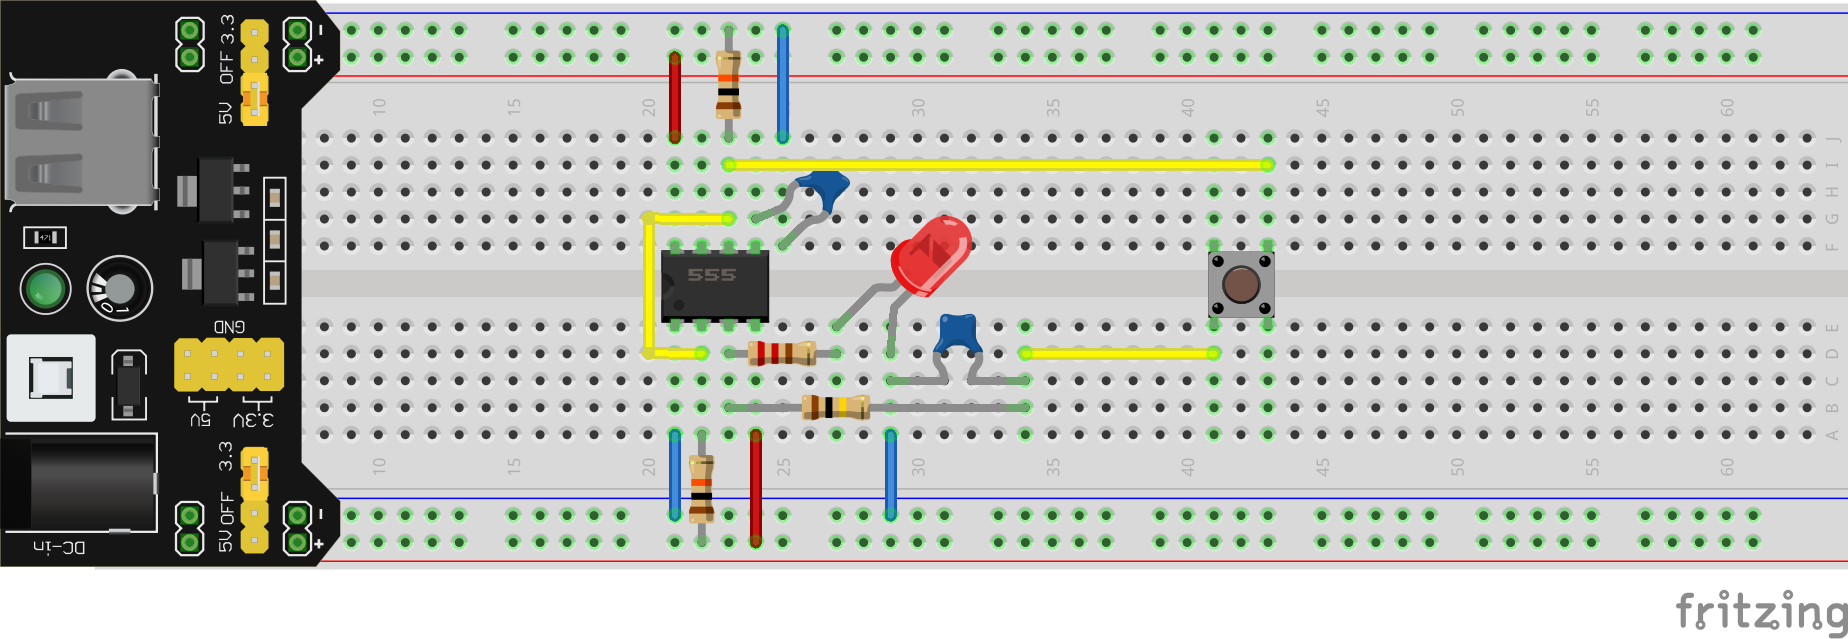
\includegraphics[width=0.8\textwidth]{lesson_circuits/L15/lesson_15.png}
    \caption{Timer Delay using 555 Breadboard Schematic}
    \label{fig:555_timer_sch}
\end{figure}
\begin{figure}[!htp]
    \centering
    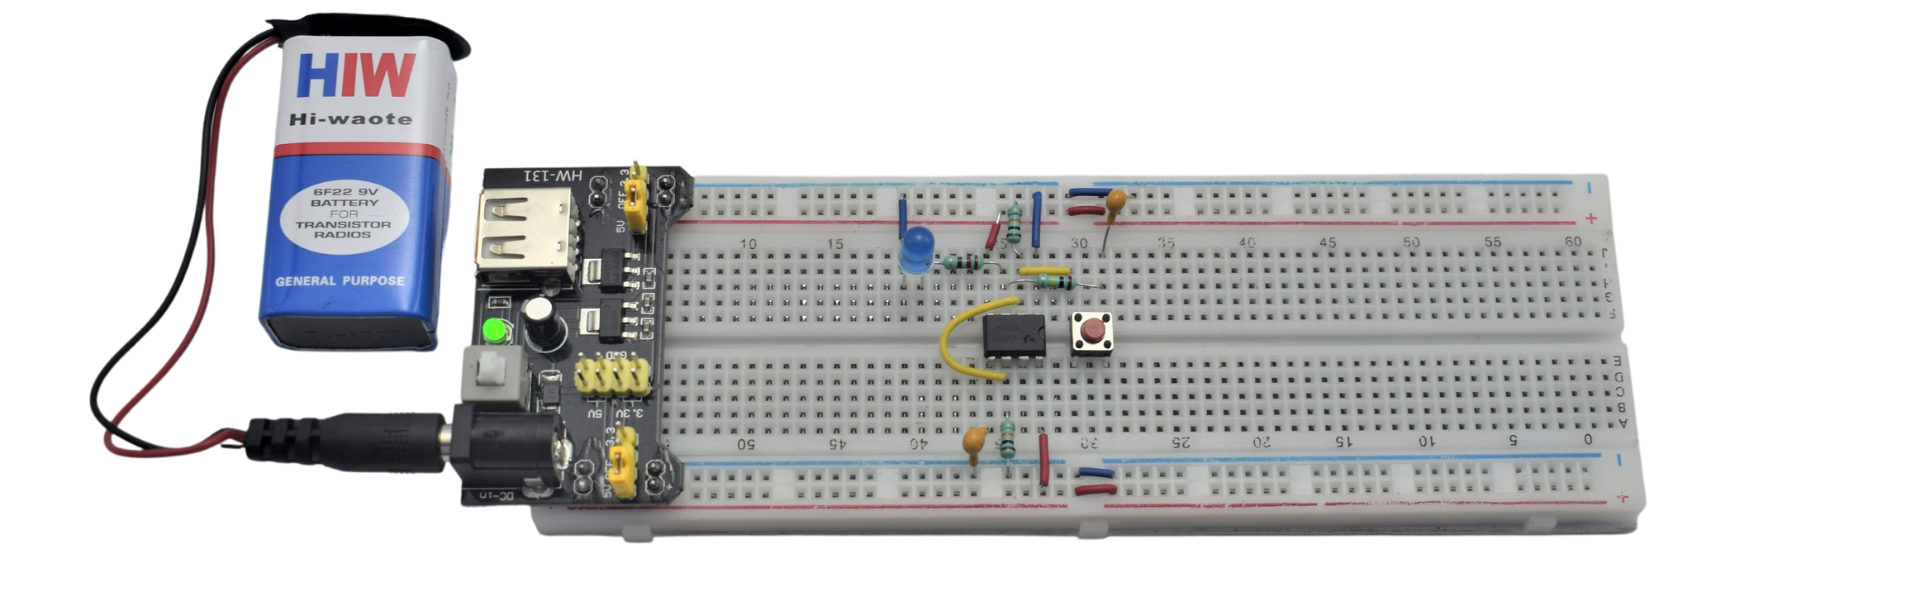
\includegraphics[width=\textwidth]{lesson_circuits/L15/L15-A.png}
    \caption{Idle}
    \label{fig:555_timer_obb}
\end{figure}
\begin{figure}[!htp]
    \centering
    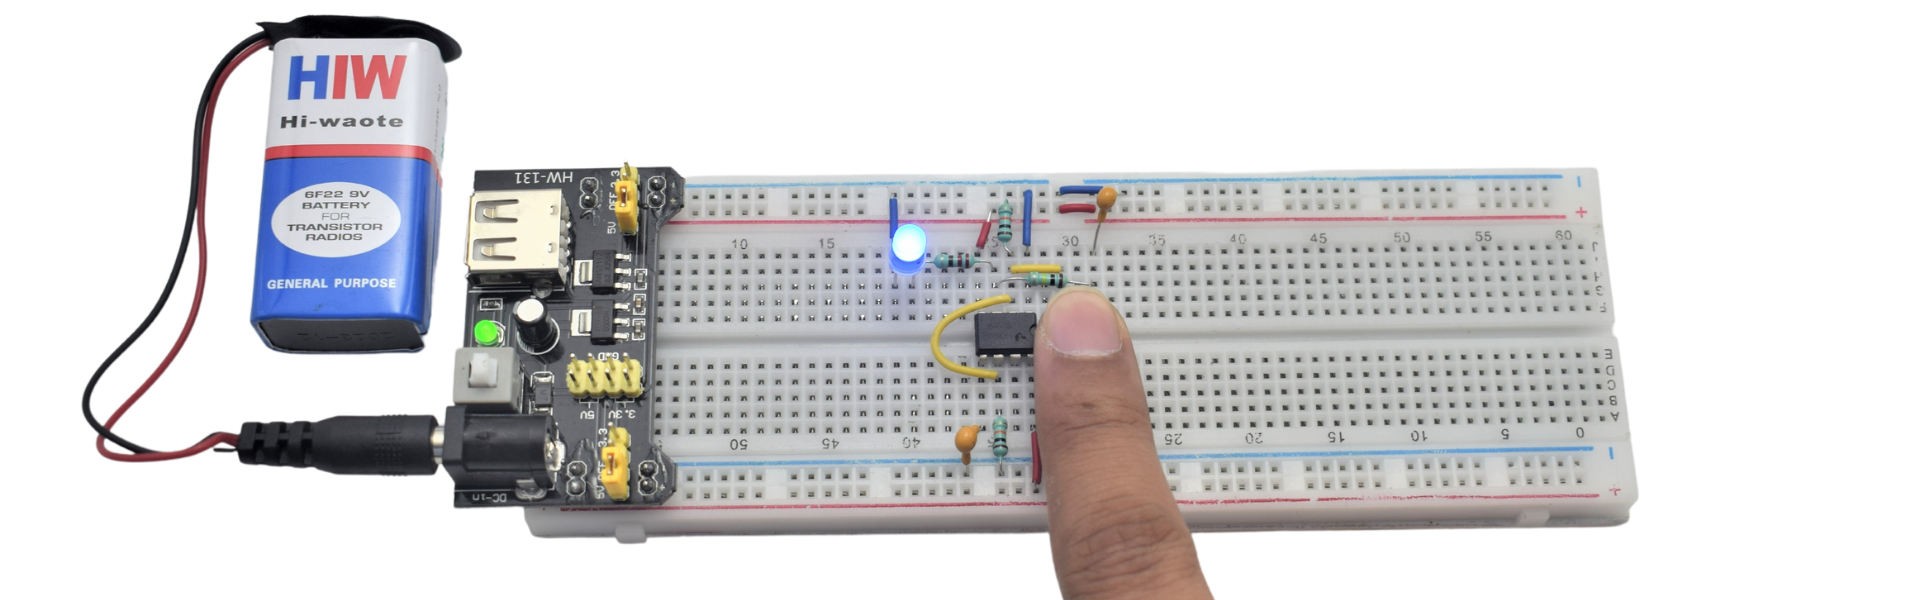
\includegraphics[width=\textwidth]{lesson_circuits/L15/L15-B.png}
    \caption{Button Pressed}
    \label{fig:555_timer_obb1}
\end{figure}
\begin{figure}[!htp]
    \centering
    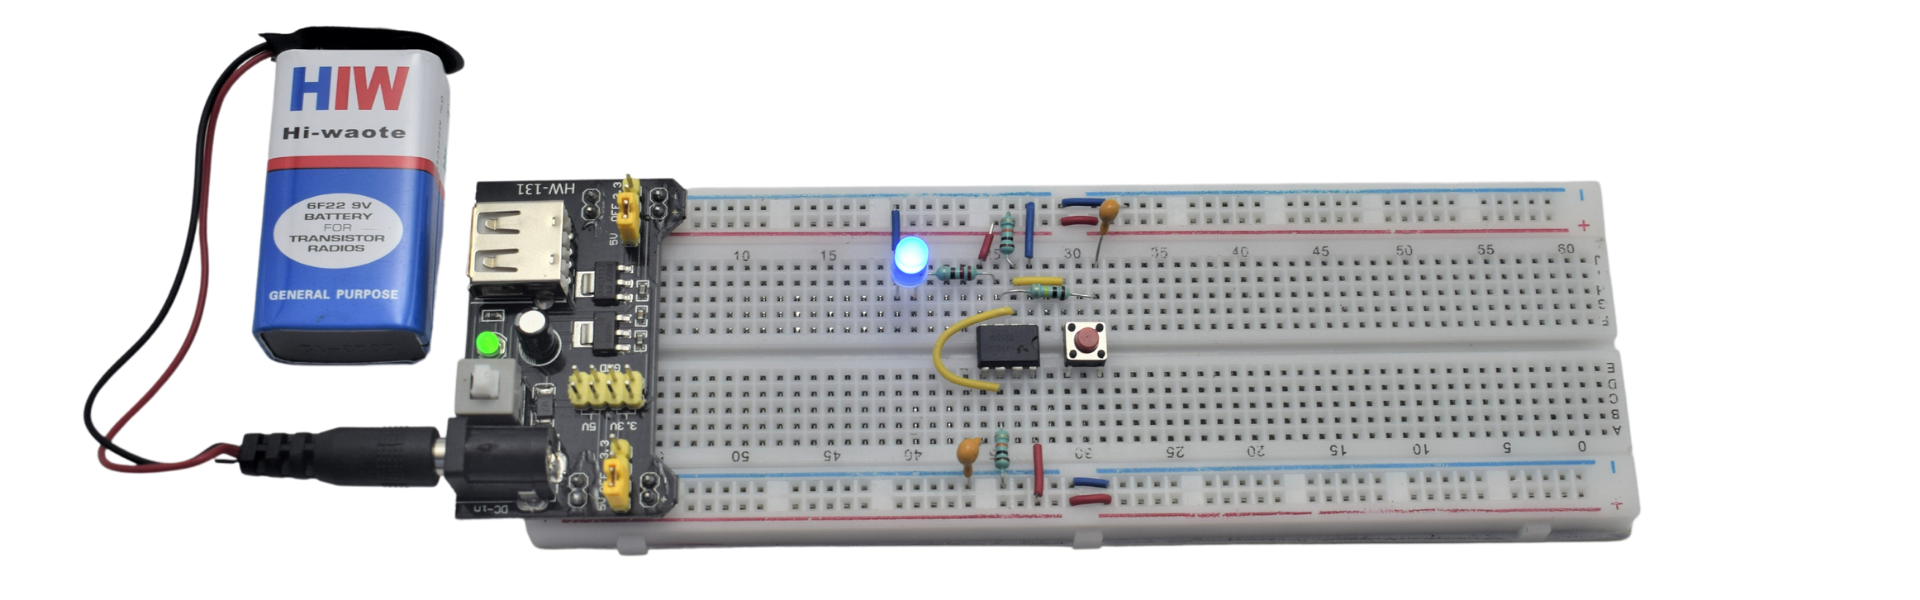
\includegraphics[width=\textwidth]{lesson_circuits/L15/L15-C.png}
    \caption{Button released}
    \label{fig:555_timer_obb2}
\end{figure}
\begin{figure}[!htp]
    \centering
    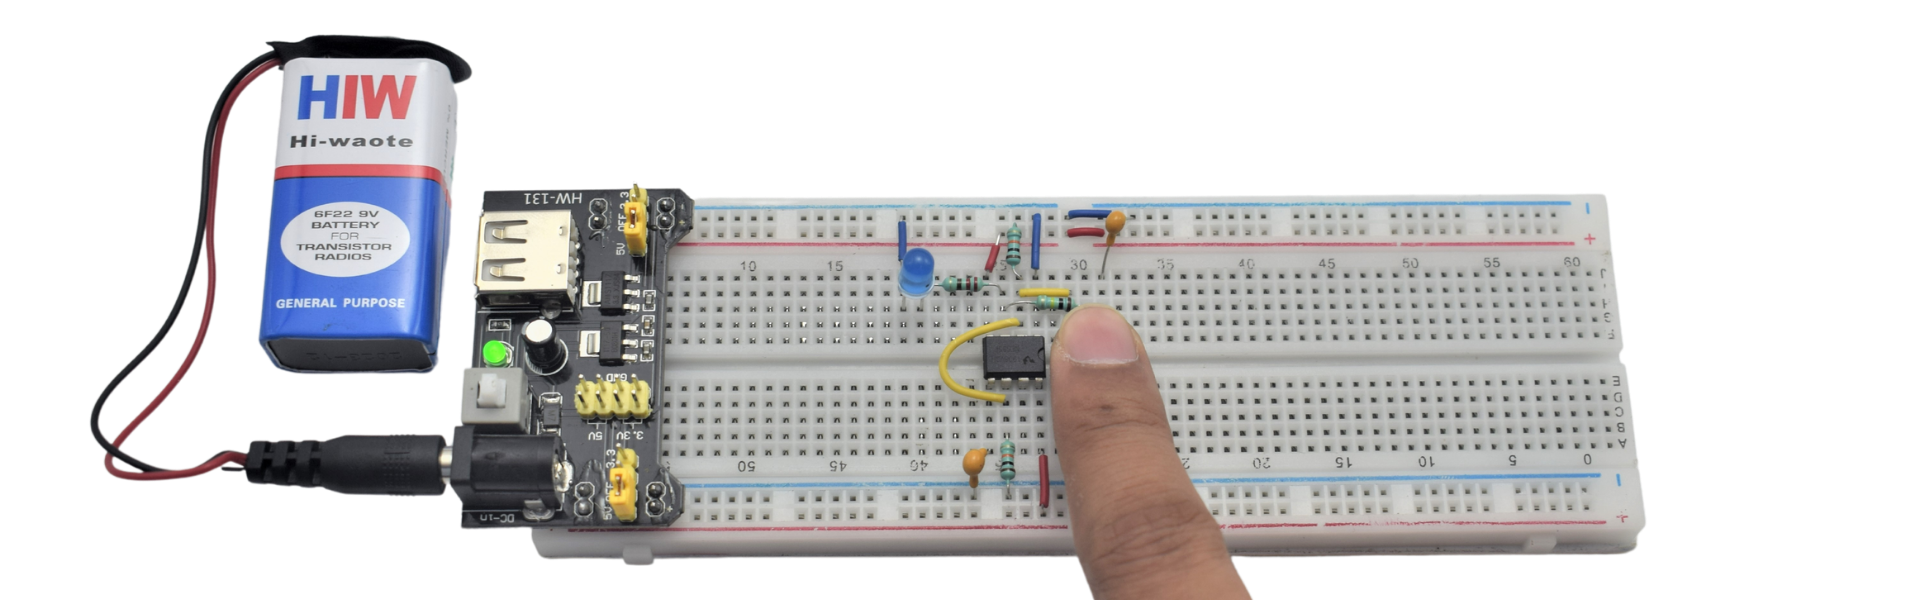
\includegraphics[width=\textwidth]{lesson_circuits/L15/L15-D.png}
    \caption{LED turned off after delay time}
    \label{fig:555_timer_obb3}
\end{figure}
\section{Lesson 17: Single Tone Buzzer with 555}
\subsection{Objective}
In this activity we'll use astable 555 circuit to produce sound using an buzzer.
\subsection{Components Required}
\begin{enumerate}
    \item Breadboard Power Supply $\times$ 1
    \item 9V Battery $\times$ 1
    \item 9V Battery Connector $\times$ 1
    \item Breadboard $\times$ 1
    \item 555 IC $\times$ 1
    \item Active Buzzer $\times$ 1
    \item \SI{10}{\kilo\ohm} $\times$ 1
    \item \SI{100}{\kilo\ohm} $\times$ 1
    \item \SI{100}{\nano\farad} $\times$ 1
    \item \SI{10}{\micro\farad} $\times$ 1
    \item Male-Male jumper wire $\times$ 7
\end{enumerate}
\subsection{Circuit}
\begin{figure}[!htp]
    \centering
    \begin{circuitikz}[scale = 1.2]
        \TIMER555(0,0){1}
        \draw (1 GND) to[short, -*] ++(0,-0.7) node[ground](g1){};
        \draw (1 CTRL) to[C, l=$100\si{\nano\farad}$] ++(0,-0.5)
            to[short, -*] ++(0,-0.2)node[](ctr){} |- (g1);
        \draw (1 VCC) to[short, -*] ++(0,0.5) node[vcc](v1){$V_{cc}$};
        \draw (1 RESET) |- (v1);
        \draw (1 THR) to[short, -*] ++(-0.5,0) node[](s6){};
        \draw (1 TRG) to[short, -*] ++(-0.5,0) node[](s2){};
        \draw (1 DIS) to[short, -*] ++(-0.5,0) node[](s7){};
        \draw (s7) to[R, l_=$10\si{\kohm}$] ($(1 THR)-(0.5,0)$);
        \draw (s7) to[R, l=$100\si{\kohm}$] ++(0,1.5) |- (v1);
        \draw (s6) -- (s2) to[C, l_=$10\si{\micro\farad}$] ++(0,-1.5) |- (g1);
        \draw (1 OUT) -- ++(0.5,0) -- ++(0,-0.5)
            to[loudspeaker, color=red] ++(0,-2.5) |- (ctr);
    \end{circuitikz}
    \caption{Single Tone Buzzer Circuit}
    \label{fig:555_sibuzz_cir}
\end{figure}
\subsection{Circuit Explanation}
In this circuit 555 is in astable mode, with a buzzer connected at the output.
\subsection{Circuit Picture}
\begin{figure}[!htp]
    \centering
    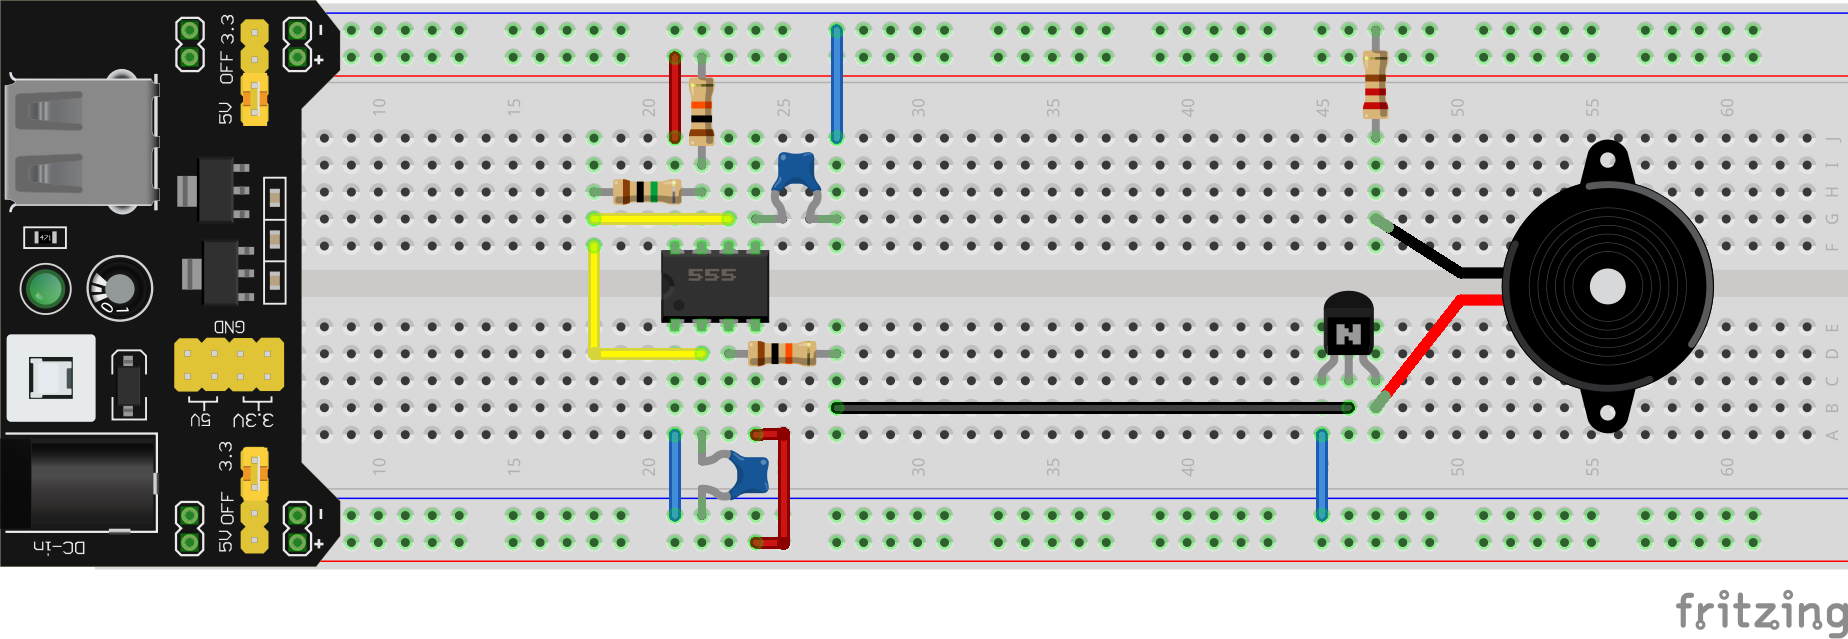
\includegraphics[width=0.8\textwidth]{lesson_circuits/L17/lesson_17.png}
    \caption{Single tone Buzzer with 555 Breadboard Schematic}
    \label{fig:555_sbuz_sch}
\end{figure}
\begin{figure}[!htp]
    \centering
    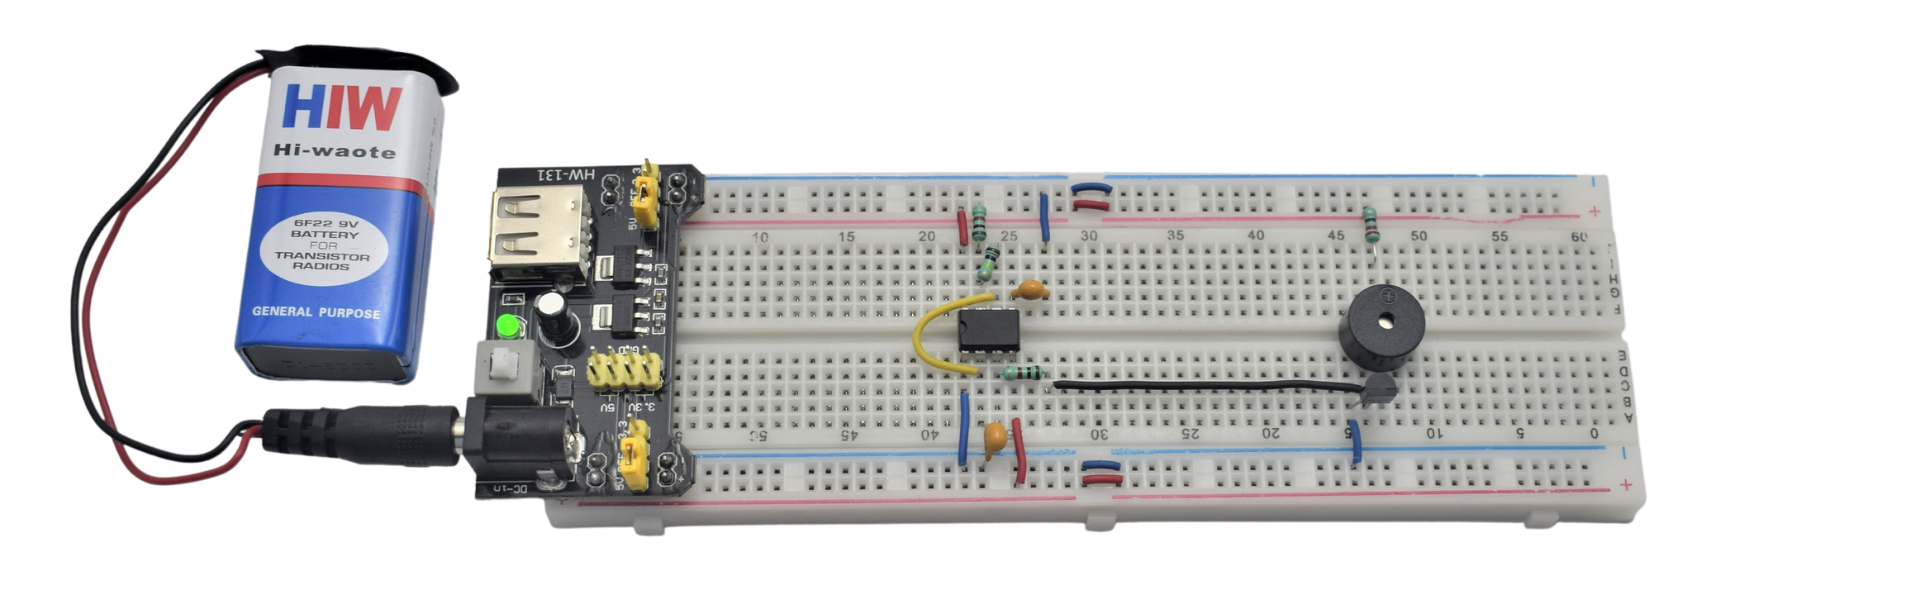
\includegraphics[width=\textwidth]{lesson_circuits/L17/L17-A.png}
    \caption{Single tone Buzzer}
    \label{fig:555_sbuz_obb}
\end{figure}
\section{Lesson 18: Short Beep}
\subsection{Objective}
In this activity we'll make a short beep sound.
\subsection{Components Required}
\begin{enumerate}
    \item Breadboard Power Supply $\times$ 1
    \item 9V Battery $\times$ 1
    \item 9V Battery Connector $\times$ 1
    \item Breadboard $\times$ 1
    \item 555 IC $\times$ 1
    \item Active Buzzer $\times$ 1
    \item 1N4007 Diode $\times$ 1
    \item \SI{10}{\kilo\ohm} $\times$ 1
    \item \SI{100}{\kilo\ohm} $\times$ 1
    \item \SI{1}{\Mohm} $\times$ 1
    \item \SI{100}{\nano\farad} $\times$ 1
    \item \SI{2.2}{\micro\farad} $\times$ 1
    \item Male-Male jumper wire $\times$ 10
\end{enumerate}
\subsection{Circuit}
\begin{figure}[!htp]
    \centering
    \begin{circuitikz}[scale = 1.2]
        \TIMER555(0,0){1}
        \draw (1 GND) to[short, -*] ++(0,-0.7) node[ground](g1){};
        \draw (1 CTRL) to[C, l=$100\si{\nano\farad}$] ++(0,-0.5)
            to[short, -*] ++(0,-0.2)node[](ctr){} |- (g1);
        \draw (1 VCC) to[short, -*] ++(0,0.5) node[vcc](v1){$V_{cc}$};
        \draw (1 RESET) |- (v1);
        \draw (1 THR) to[short, -*] ++(-0.5,0) node[](s6){};
        \draw (1 TRG) to[short, -*] ++(-0.5,0) node[](s2){};
        \draw (1 DIS) to[short, -*] ++(-0.5,0) node[](s7){};
        \draw (s7) to[R, l_=$1\si{\Mohm}$] ($(1 THR)-(0.5,0)$);
        \draw (s7) to[R, l=$10\si{\kohm}$] ++(0,1.5) |- (v1);
        \draw (s6) -- (s2) to[C, l_=$2.2\si{\micro\farad}$] ++(0,-1.5) |- (g1);
        \draw (1 OUT) -- ++(0.5,0) -- ++(0,-0.5)
            to[loudspeaker, color=red] ++(0,-2.5) |- (ctr);
        \draw (s7) -- ++(-1.5,0)
            to[R, l_=$100\si{\kohm}$] ++(0,-1.5)
            to[empty diode] ++(0,-1.5) |- (s2);
    \end{circuitikz}
    \caption{Short Beep Circuit}
    \label{fig:555_shbeep_cir}
\end{figure}
\subsection{Circuit Explanation}
In circuit is similar to the one explained in section \ref{astablemode}. In this circuit when the output is high, the capacitor 
get charged via the $100\si{\kohm}$ resistor and diode instead of $1\si{\Mohm}$, therefore it charges very rapidly.
\begin{figure}[!htp]
    \centering
    \begin{circuitikz}[scale = 1.2]
        \TIMER555(0,0){1}
        \draw (1 GND) to[short, -*] ++(0,-0.7) node[ground](g1){};
        \draw (1 CTRL) to[C, l=$100\si{\nano\farad}$] ++(0,-0.5)
            to[short, -*] ++(0,-0.2)node[](ctr){} |- (g1);
        \draw (1 VCC) to[short, -*] ++(0,0.5) node[vcc](v1){$V_{cc}$};
        \draw (1 RESET) |- (v1);
        \draw (1 THR) to[short, -*] ++(-0.5,0) node[](s6){};
        \draw (1 TRG) to[short, -*] ++(-0.5,0) node[](s2){};
        \draw (1 DIS) to[short, -*] ++(-0.5,0) node[](s7){};
        \draw (s7) to[R, l_=$1\si{\Mohm}$] ($(1 THR)-(0.5,0)$);
        \draw (s7) to[R, l=$10\si{\kohm}$] ++(0,1.5) |- (v1);
        \draw (s6) -- (s2) to[C, l_=$2.2\si{\micro\farad}$] ++(0,-1.5) |- (g1);
        \draw (1 OUT) -- ++(0.5,0) -- ++(0,-0.5)
            to[loudspeaker, color=red] ++(0,-2.5) |- (ctr);
        \draw (s7) -- ++(-1.5,0)
            to[R, l_=$100\si{\kohm}$] ++(0,-1.5)
            to[empty diode] ++(0,-1.5) |- (s2);
        \draw[->, red]
            ($(v1)+(-0.2,0.2)$) -- ++(-2,0) -- ++(0,-2) -- ++(-1.4,0)
            -- ++(0,-2.5) -- ++(0.6,0) -- ++(0,-0.4);
    \end{circuitikz}
    \caption{Short Beep Circuit : Capacitor Charging}
    \label{fig:555_shbeep_charge_cir}
\end{figure}

And when the output is low, it discharges through $1\si{\Mohm}$ resistor. Since the high time is very less compared to the 
low time, the buzzer produces a short beep tone.
\begin{figure}[!htp]
    \centering
    \begin{circuitikz}[scale = 1.2]
        \TIMER555(0,0){1}
        \draw (1 GND) to[short, -*] ++(0,-0.7) node[ground](g1){};
        \draw (1 CTRL) to[C, l=$100\si{\nano\farad}$] ++(0,-0.5)
            to[short, -*] ++(0,-0.2)node[](ctr){} |- (g1);
        \draw (1 VCC) to[short, -*] ++(0,0.5) node[vcc](v1){$V_{cc}$};
        \draw (1 RESET) |- (v1);
        \draw (1 THR) to[short, -*] ++(-0.5,0) node[](s6){};
        \draw (1 TRG) to[short, -*] ++(-0.5,0) node[](s2){};
        \draw (1 DIS) to[short, -*] ++(-0.5,0) node[](s7){};
        \draw (s7) to[R, l_=$1\si{\Mohm}$] ($(1 THR)-(0.5,0)$);
        \draw (s7) to[R, l=$10\si{\kohm}$] ++(0,1.5) |- (v1);
        \draw (s6) -- (s2) to[C, l_=$2.2\si{\micro\farad}$] ++(0,-1.5) |- (g1);
        \draw (1 OUT) -- ++(0.5,0) -- ++(0,-0.5)
            to[loudspeaker, color=red] ++(0,-2.5) |- (ctr);
        \draw (s7) -- ++(-1.5,0)
            to[R, l_=$100\si{\kohm}$] ++(0,-1.5)
            to[empty diode] ++(0,-1.5) |- (s2);
        \draw[<-, blue]
            ($(1 DIS)-(0.2,0.2)$) -- ++(-0.5,0) -- ++(0,-3.2);
    \end{circuitikz}
    \caption{Short Beep Circuit : Capacitor Discharging}
    \label{fig:555_shbeep_discharge_cir}
\end{figure}

\subsection{Circuit Picture}
\begin{figure}[!htp]
    \centering
    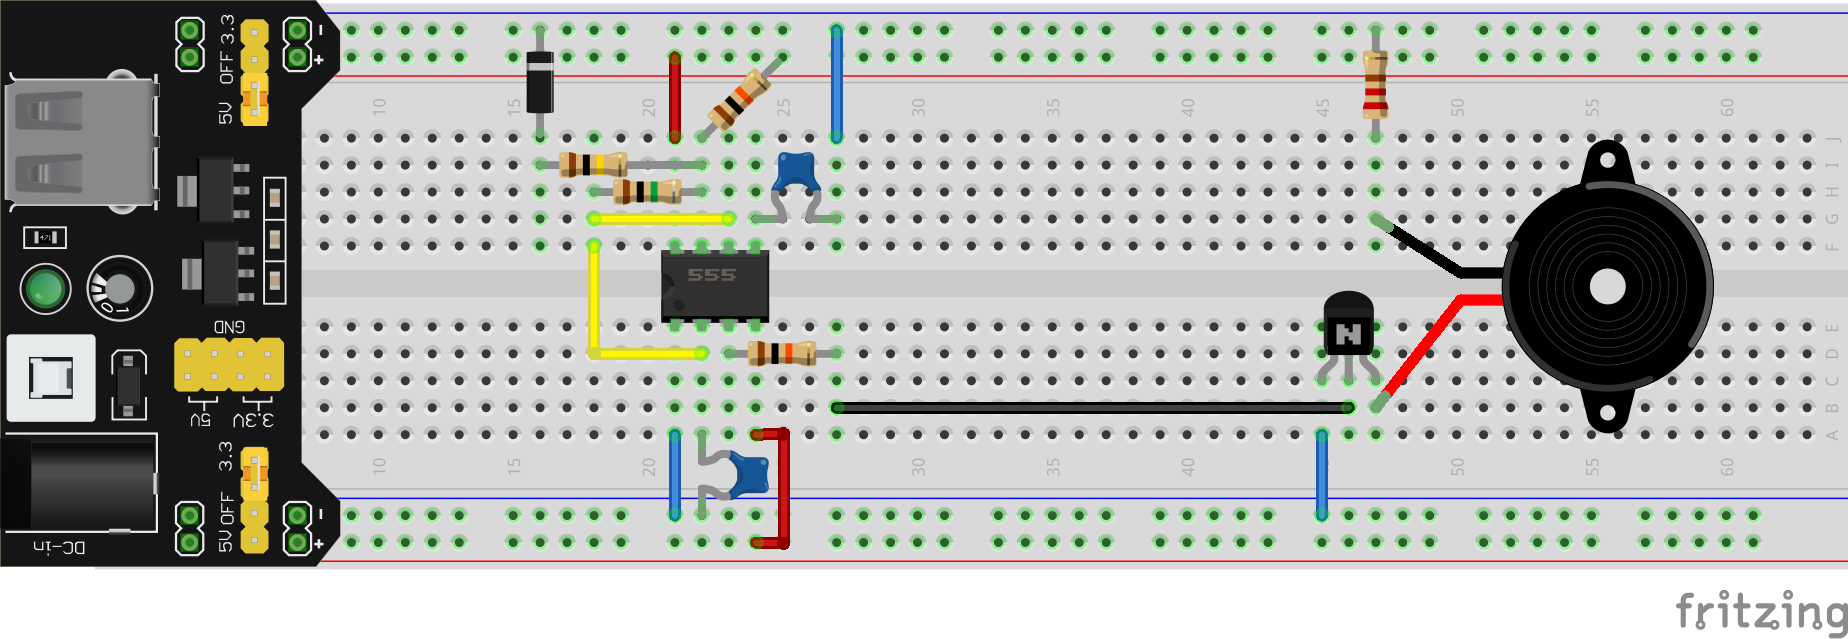
\includegraphics[width=0.8\textwidth]{lesson_circuits/L18/lesson_18.png}
    \caption{Short Beep using 555 Breadboard Schematic}
    \label{fig:555_sbeep_sch}
\end{figure}
\begin{figure}[!htp]
    \centering
    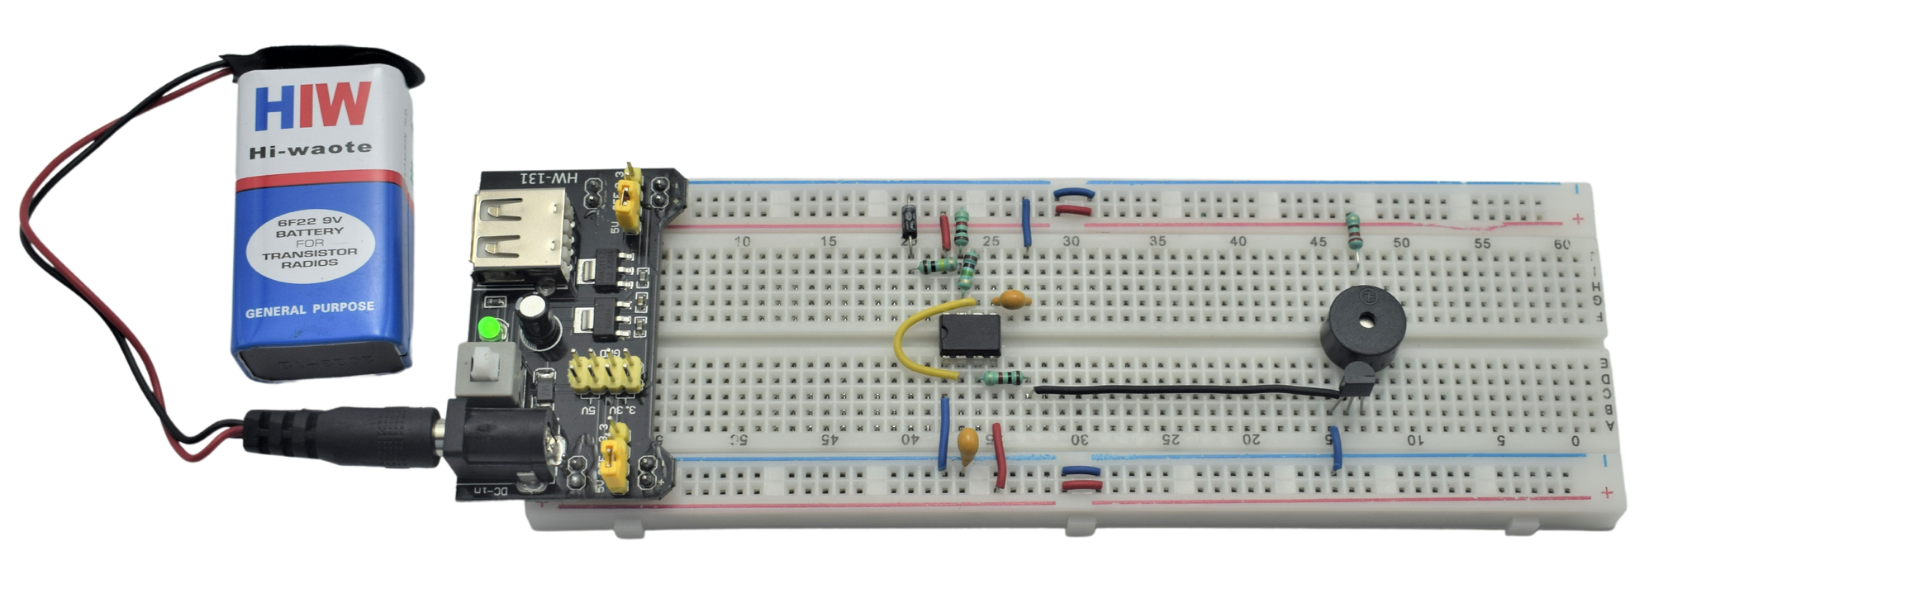
\includegraphics[width=\textwidth]{lesson_circuits/L18/L18-A.png}
    \caption{Short Beep}
    \label{fig:555_sbeep_obb}
\end{figure}
\section{Lesson 19: Break Beam Detector using 555 and LDR}
\subsection{Objective}
In this activity we'll make a break beam detector circuit.
\subsection{Components Required}
\begin{enumerate}
    \item Breadboard Power Supply $\times$ 1
    \item 9V Battery $\times$ 1
    \item 9V Battery Connector $\times$ 1
    \item Breadboard $\times$ 1
    \item 555 IC $\times$ 1
    \item Passive Buzzer $\times$ 1
    \item White LED $\times$ 1
    \item LDR $\times$ 1
    \item \SI{220}{\ohm} $\times$ 1
    \item \SI{10}{\kilo\ohm} $\times$ 3
    \item \SI{100}{\nano\farad} $\times$ 2
    \item \SI{10}{\micro\farad} $\times$ 1
    \item Male-Male jumper wire $\times$ 15
\end{enumerate}
\subsection{Circuit}
\begin{figure}[!htp]
    \centering
    \begin{circuitikz}[scale = 1.2]
        \TIMER555(0,0){1}
        \draw (0,-3.5) node[npn](t1){T1};
        \draw (1 GND) -- (t1.C);
        \draw (t1.E) -- ++(0,-0.2) node[circ](g1){} -- node[ground](g1){} ++(0,0);
        \draw (1 CTRL) to[C, l=$100\si{\nano\farad}$] ++(0,-0.5)
            to[short, -*] ++(0,-0.2)node[](ctr){} |- (g1);
        \draw (1 VCC) to[short, -*] ++(0,0.5) node[vcc](v1){$V_{cc}$};
        \draw (1 RESET) |- (v1);
        \draw (1 THR) to[short, -*] ++(-0.5,0) node[](s6){};
        \draw (1 TRG) to[short, -*] ++(-0.5,0) node[](s2){};
        \draw (1 DIS) to[short, -*] ++(-0.5,0) node[](s7){};
        \draw (s7) to[R, l_=$10\si{\kohm}$] ($(1 THR)-(0.5,0)$);
        \draw (s7) to[R, l=$100\si{\kohm}$] ++(0,1.5)node[circ](sh1){} |- (v1);
        \draw (s6) -- (s2) to[C, l_=$10\si{\micro\farad}$] ++(0,-1.5) |- (g1);
        \draw (1 OUT) -- ++(0.5,0) -- ++(0,-0.5) 
            to[C, l=$10\si{\uF}$] ++ (0,-1)
            to[loudspeaker] ++(0,-1.5) |- (ctr);
        \draw (-4,0) node[npn](t2){T2};
        \draw (t1.B) -| (t2.E);
        \draw (t2.C) -- ++(0,2.35)node[circ](t2c){} |- (sh1);
        \draw (t2.B) -- ++(-1,0)node[circ](t2b){};
        \draw (t2c) -- ++(-1.7,0)node[circ](ab){} to[R, l=$10\si{\kohm}$] (t2b)
            to[sR] ++(0,-4.35)node[circ](g3){} to[short,-*] ++(3.2,0);
        \draw (ab) -- ++(-1,0) to[R, l_=$220\si{\ohm}$] ++(0,-3) to[empty led] ++(0,-4) |- (g3);
    \end{circuitikz}
    \caption{Break Beam Detector Circuit}
    \label{fig:555_bbdet_cir}
\end{figure}
\subsection{Circuit Explanation}
When there is no barrier in between the LED and LDR, the resistance of LDR is very low and there the base transistor $T2$ is near 
ground potential or 0 volt and is in cut-off mode. Since, $T2$ is off, $T1$ is also off and the 555 will not work, because the GND 
pin is connected to collector of $T1$.

When there is obstruction between light and LDR, the resistance of LDR goes high, turning the $T2$ on, which turns on the $T1$. 
Now $T1$ is and 555 will start operating in astable mode.
\subsection{Circuit Picture}
\begin{figure}[!htp]
    \centering
    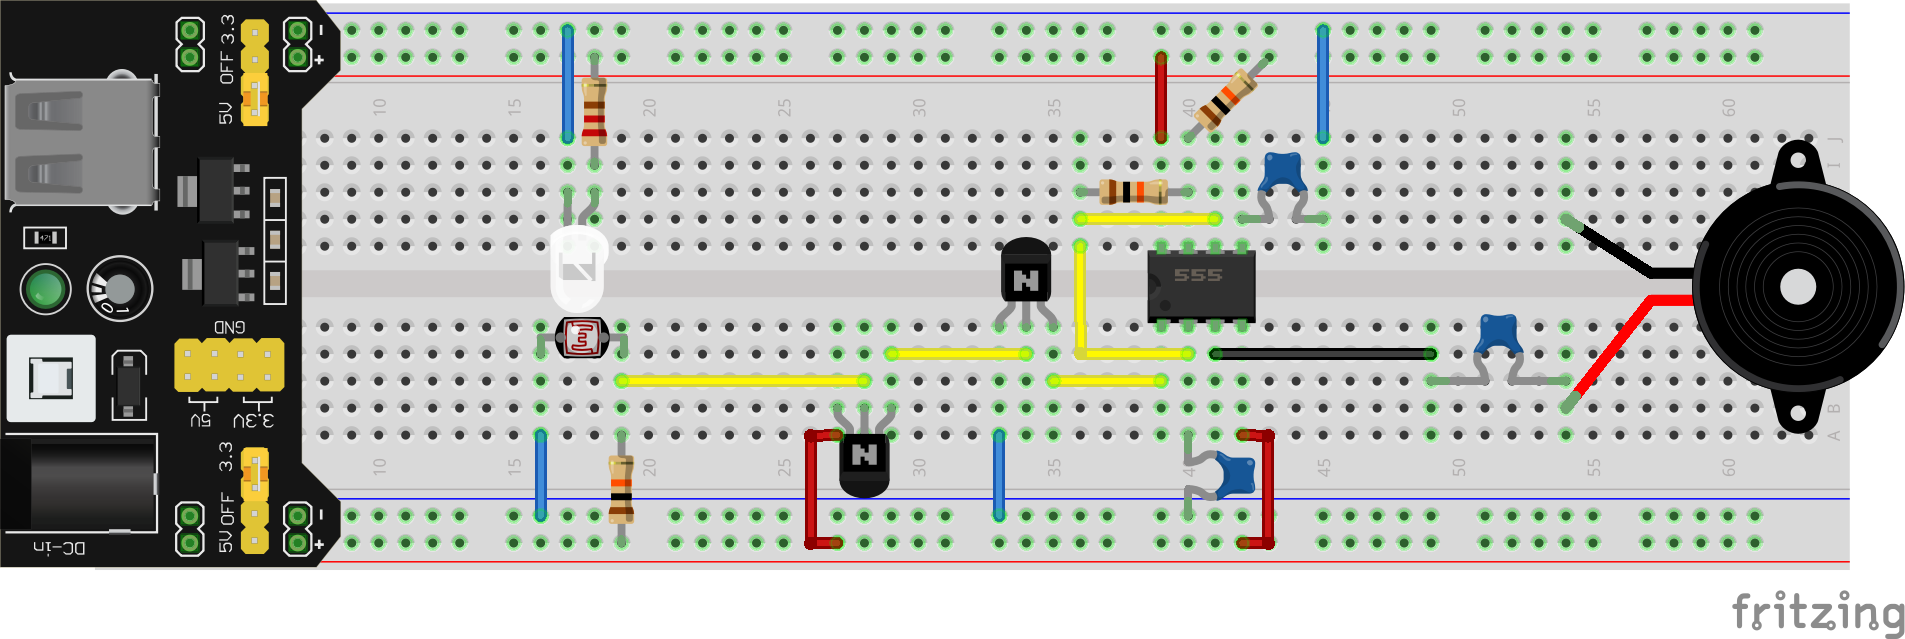
\includegraphics[width=0.8\textwidth]{lesson_circuits/L19/lesson_19.png}
    \caption{Break Beam Detector using 555 and LDR Breadboard Schematic}
    \label{fig:555_bbdet_sch}
\end{figure}
\begin{figure}[!htp]
    \centering
    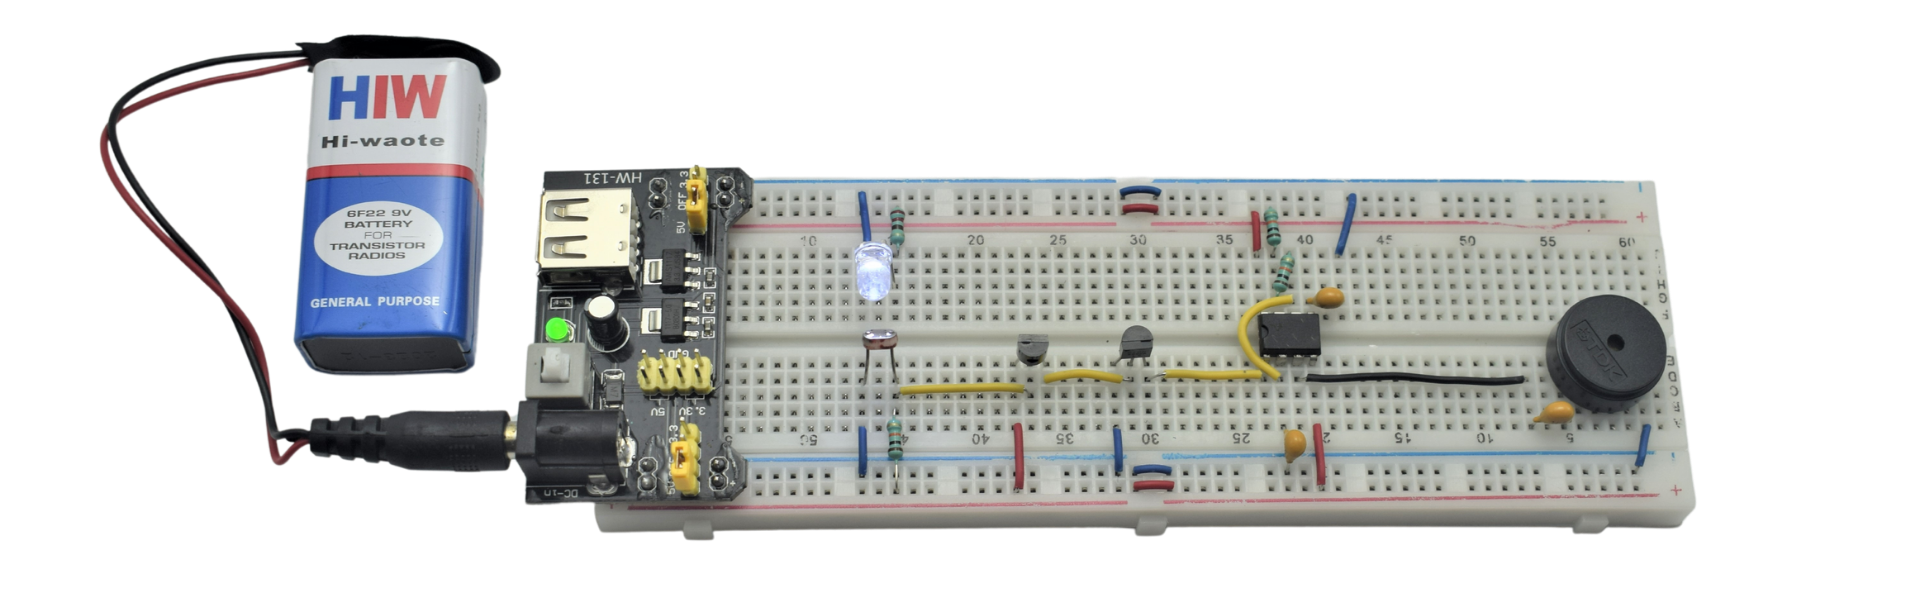
\includegraphics[width=\textwidth]{lesson_circuits/L19/L19-A.png}
    \caption{No Obstacle: Buzzer OFF}
    \label{fig:555_bbdet_obb}
\end{figure}
\begin{figure}[!htp]
    \centering
    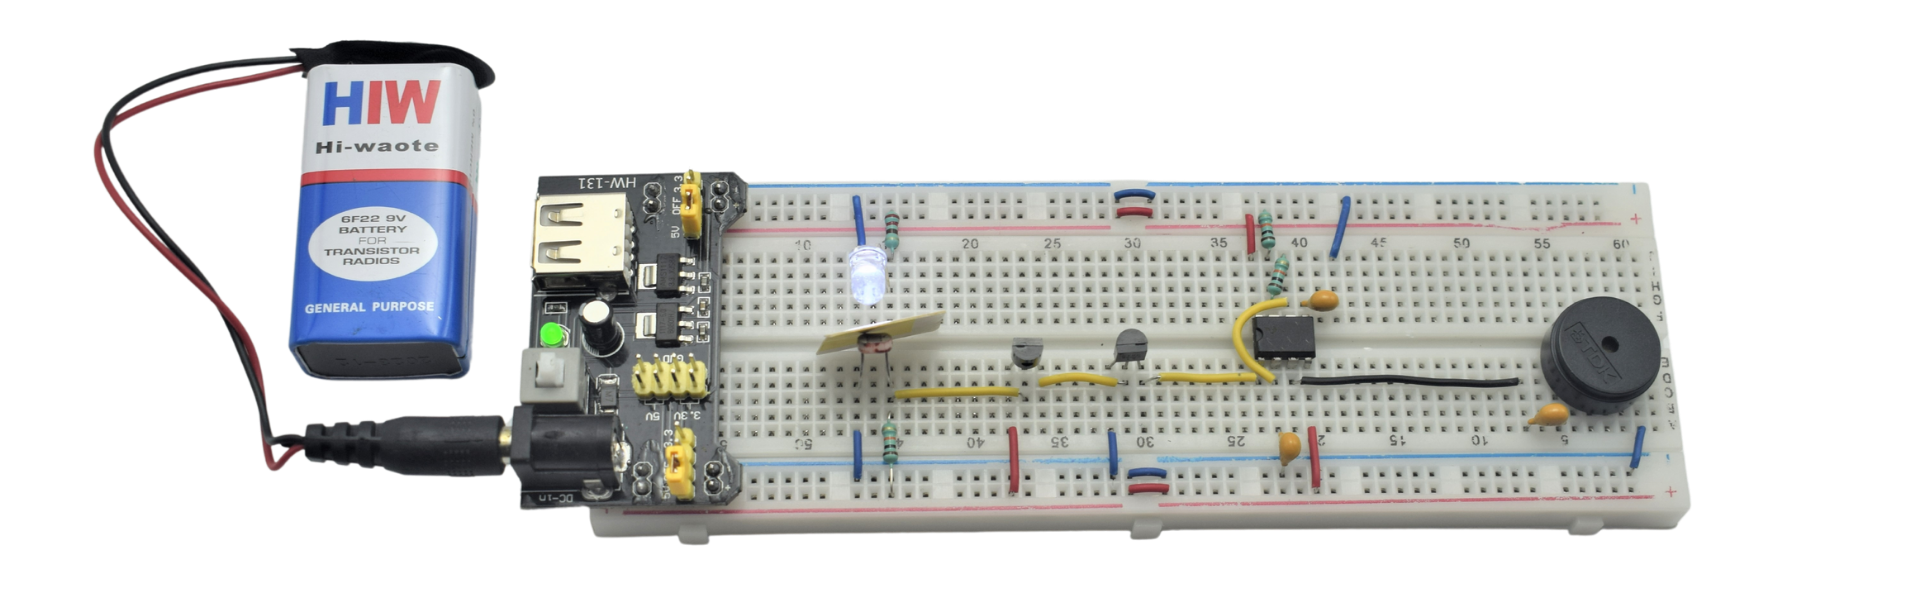
\includegraphics[width=\textwidth]{lesson_circuits/L19/L19-B.png}
    \caption{Obstacle: Buzzer ON}
    \label{fig:555_bbdet_obb1}
\end{figure}
\section{Lesson 20: Light reactive buzzer using 555 and LDR}
\subsection{Objective}
In this activity we'll make a light reactive tone generator.
\subsection{Components Required}
\begin{enumerate}
    \item Breadboard Power Supply $\times$ 1
    \item 9V Battery $\times$ 1
    \item 9V Battery Connector $\times$ 1
    \item Breadboard $\times$ 1
    \item 555 IC $\times$ 1
    \item Passive Buzzer $\times$ 1
    \item LDR $\times$ 1
    \item \SI{10}{\kilo\ohm} $\times$ 1
    \item \SI{100}{\nano\farad} $\times$ 2
    \item \SI{10}{\micro\farad} $\times$ 1
    \item Male-Male jumper wire $\times$ 9
\end{enumerate}
\subsection{Circuit}
\begin{figure}[!htp]
    \centering
    \begin{circuitikz}[scale = 1.2]
        \TIMER555(0,0){1}
        \draw (1 GND) to[short, -*] ++(0,-0.7) node[ground](g1){};
        \draw (1 CTRL) to[C, l=$100\si{\nano\farad}$] ++(0,-0.5)
            to[short, -*] ++(0,-0.2)node[](ctr){} |- (g1);
        \draw (1 VCC) to[short, -*] ++(0,0.5) node[vcc](v1){$V_{cc}$};
        \draw (1 RESET) |- (v1);
        \draw (1 THR) to[short, -*] ++(-0.5,0) node[](s6){};
        \draw (1 TRG) to[short, -*] ++(-0.5,0) node[](s2){};
        \draw (1 DIS) to[short, -*] ++(-0.5,0) node[](s7){};
        \draw (s7) to[sR] ($(1 THR)-(0.5,0)$);
        \draw (s7) to[R, l=$100\si{\kohm}$] ++(0,1.5) |- (v1);
        \draw (s6) -- (s2) to[C, l_=$10\si{\micro\farad}$] ++(0,-1.5) |- (g1);
        \draw (1 OUT) -- ++(0.5,0) -- ++(0,-0.5) 
            to[C, l=$10\si{\uF}$] ++ (0,-1)
            to[loudspeaker] ++(0,-1.5) |- (ctr);
    \end{circuitikz}
    \caption{Light Reactive Buzzer Circuit}
    \label{fig:555_lrbuzz_cir}
\end{figure}
\subsection{Circuit Explanation}
In this circuit the 555 is in astable mode, but the $R_2$ resistor is replaced with an LDR, so according to the change in intensity 
of light falling on the LDR, the frequency of output is changed, changing the tone generated by the buzzer.
\subsection{Circuit Picture}
\begin{figure}[!htp]
    \centering
    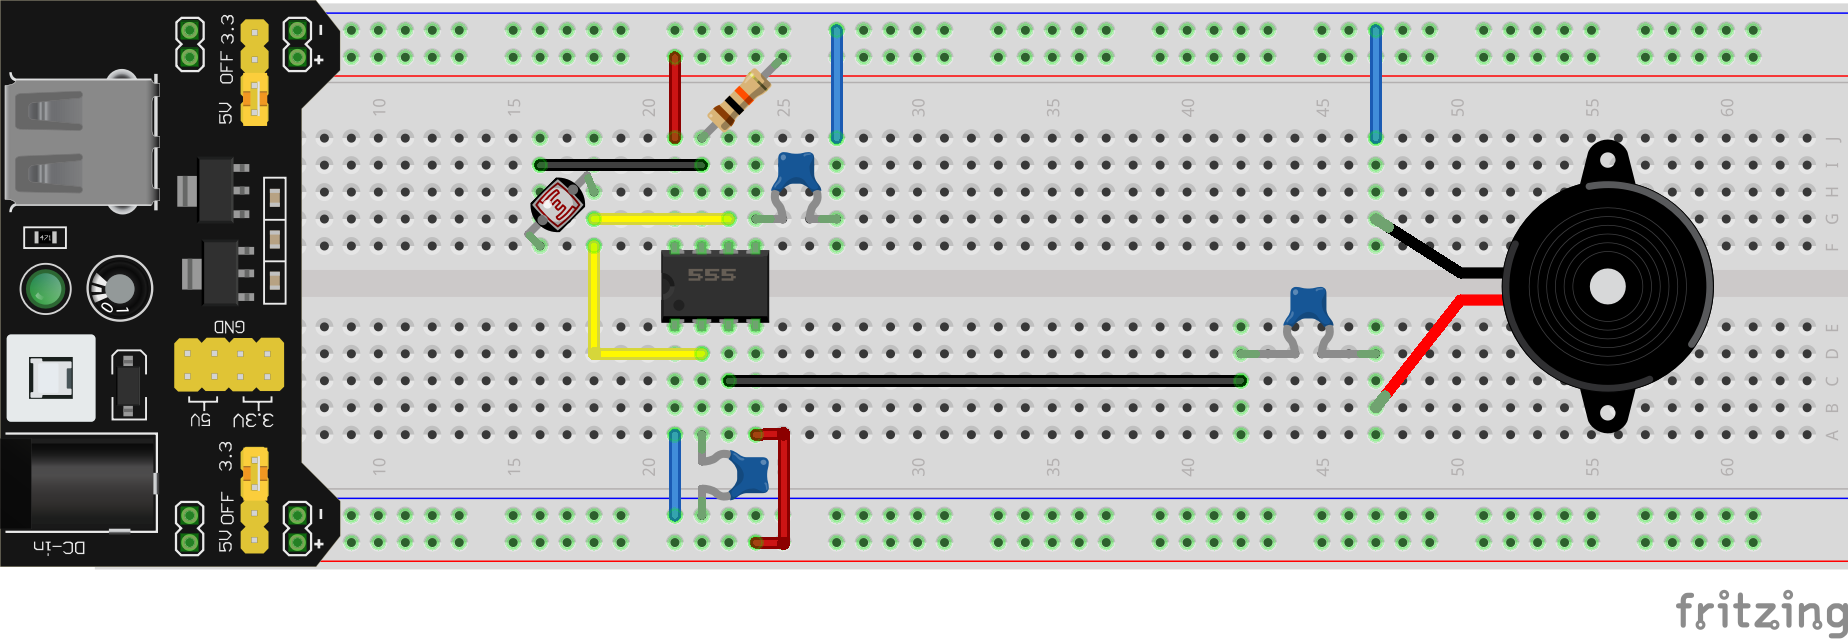
\includegraphics[width=0.8\textwidth]{lesson_circuits/L20/lesson_20.png}
    \caption{Light reactive Buzzer Breadboard Schematic}
    \label{fig:555_ldrbuzz_sch}
\end{figure}
\begin{figure}[!htp]
    \centering
    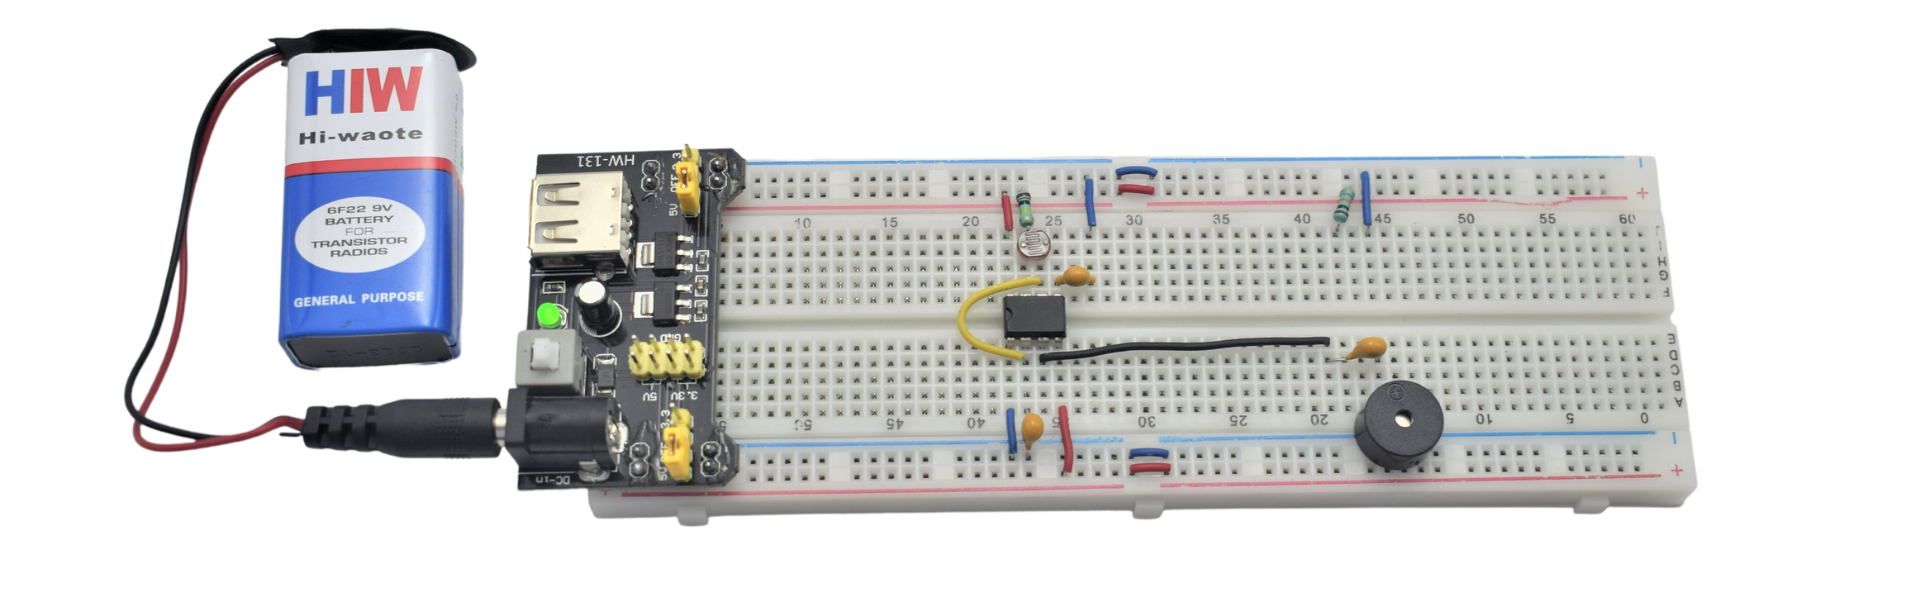
\includegraphics[width=\textwidth]{lesson_circuits/L20/L20-A.png}
    \caption{Light reactive Buzzer}
    \label{fig:555_ldrbuzz_obb}
\end{figure}
\section{Lesson 21: Audio Tone/Siren}
\subsection{Objective}
In this activity we'll make an audio tone/siren generator.
\subsection{Components Required}
\begin{enumerate}
    \item Breadboard Power Supply $\times$ 1
    \item 9V Battery $\times$ 1
    \item 9V Battery Connector $\times$ 1
    \item Breadboard $\times$ 1
    \item 555 IC $\times$ 2
    \item Passive Buzzer $\times$ 1
    \item \SI{10}{\kilo\ohm} $\times$ 5
    \item \SI{100}{\kilo\ohm} $\times$ 1
    \item \SI{100}{\nano\farad} $\times$ 2
    \item \SI{10}{\micro\farad} $\times$ 2
    \item Male-Male jumper wire $\times$ 14
\end{enumerate}
\subsection{Circuit}
\begin{figure}[!htp]
    \centering
    \begin{circuitikz}[scale = 1]
        \TIMER555(0,0){1}
        \draw (1 GND) to[short, -*] ++(0,-0.7) node[ground](g1){};
        \draw (1 CTRL) to[C, l=$100\si{\nano\farad}$] ++(0,-0.5)
            to[short, -*] ++(0,-0.2)node[](ctr){} |- (g1);
        \draw (1 VCC) to[short, -*] ++(0,0.5) node[vcc](v1){$V_{cc}$};
        \draw (1 RESET) |- (v1);
        \draw (1 THR) to[short, -*] ++(-0.5,0) node[](s6){};
        \draw (1 TRG) to[short, -*] ++(-0.5,0) node[](s2){};
        \draw (1 DIS) to[short, -*] ++(-0.5,0) node[](s7){};
        \draw (s7) to[R, l_=$10\si{\kohm}$] ($(1 THR)-(0.5,0)$);
        \draw (s7) to[R, l=$100\si{\kohm}$] ++(0,1.5) |- (v1);
        \draw (s6) -- (s2) to[C, l_=$10\si{\micro\farad}$] ++(0,-1.5) |- (g1);
        
        \TIMER555(8,0){2};
        \draw (2 GND) to[short, -*] ++(0,-0.7) node[ground](g21){};
        \draw (2 VCC) to[short, -*] ++(0,0.5) node[vcc](v21){$V_{cc}$};
        \draw (2 RESET) |- (v21);
        \draw (2 THR) to[short, -*] ++(-0.5,0) node[](s26){};
        \draw (2 TRG) to[short, -*] ++(-0.5,0) node[](s22){};
        \draw (2 DIS) to[short, -*] ++(-0.5,0) node[](s27){};
        \draw (s27) to[R, l=$10\si{\kohm}$] ($(2 THR)-(0.5,0)$);
        \draw (s27) to[R, l=$100\si{\kohm}$] ++(0,1.5) |- (v21);
        \draw (s26) -- (s22) to[C, l_=$10\si{\micro\farad}$] ++(0,-1.5) |- (g21);
        \draw (2 OUT) -- ++(0.5,0) -- ++(0,-0.5) 
            to[C, l=$10\si{\uF}$] ++ (0,-1)
            to[loudspeaker] ++(0,-1.5) |- (g21);
        \draw (2 CTRL) -- ++(0,-0.2) -- ++(-5.5,0) 
            to[R, l=$10\si{\kohm}$] ++(0,2) |- (1 OUT);
    \end{circuitikz}
    \caption{Audio Tone/Siren Circuit}
    \label{fig:555_ausiren_cir}
\end{figure}
\subsection{Circuit Explanation}
In this circuit both the 555 are running in astable. But, we are controlling the input voltage of the second 555 using the output 
of the first, such that whenever the output of first 555 changes, the frequency of output of second 555 changes, producing two 
different tone after each interval. 
\subsection{Circuit Picture}
\begin{figure}[!htp]
    \centering
    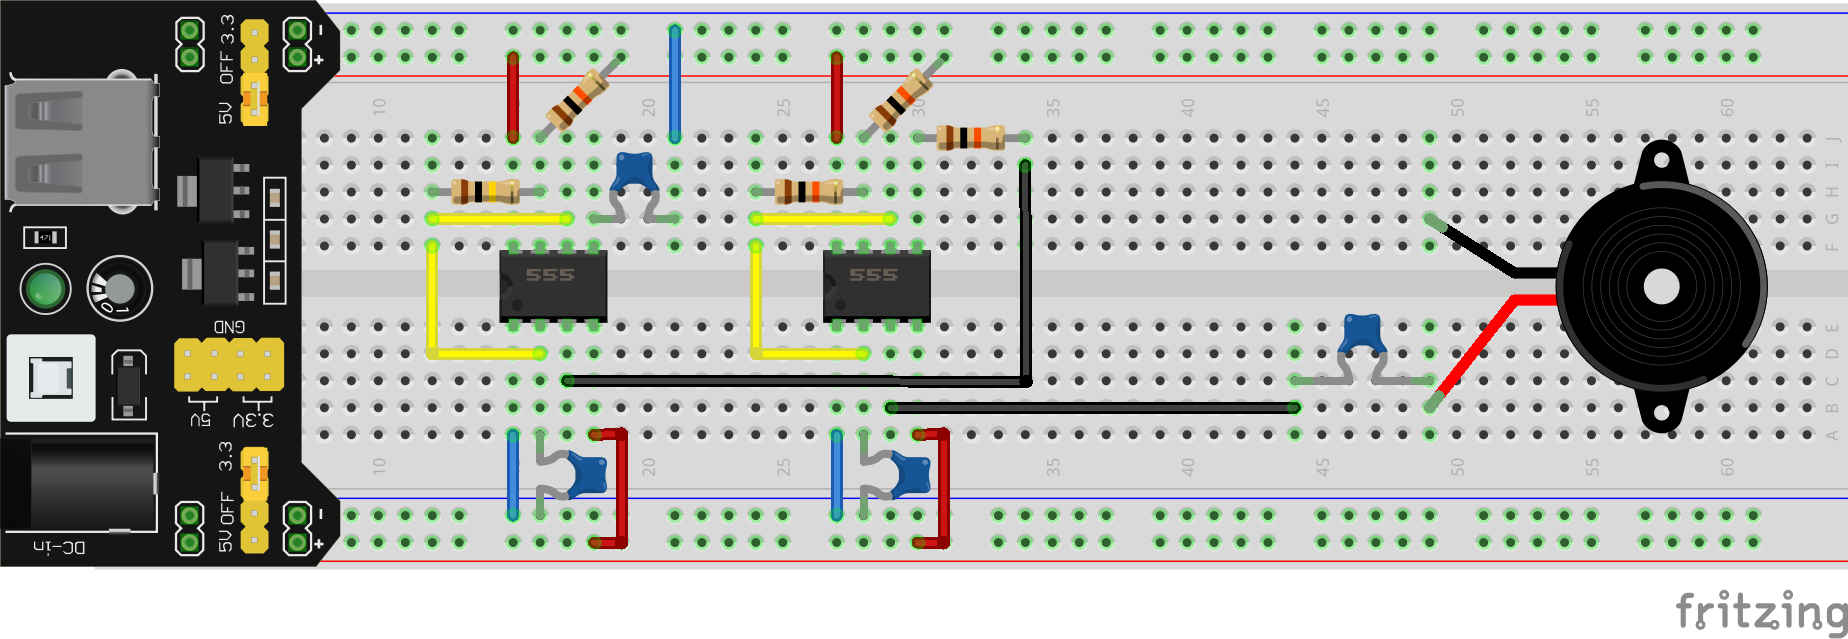
\includegraphics[width=0.8\textwidth]{lesson_circuits/L21/lesson_21.png}
    \caption{Audio Tone/Siren Breadboard Schematic}
    \label{fig:555_audsi_sch}
\end{figure}
\begin{figure}[!htp]
    \centering
    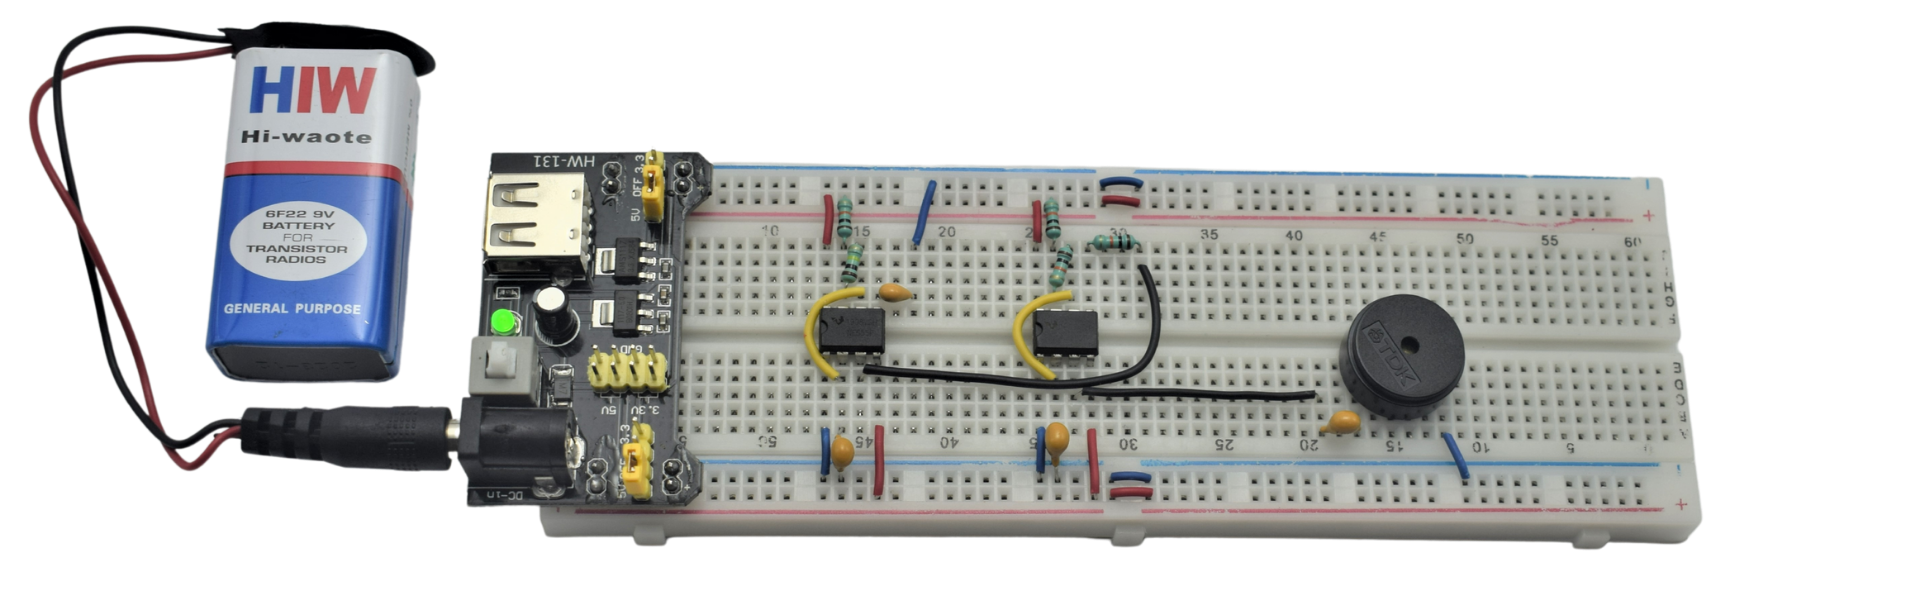
\includegraphics[width=\textwidth]{lesson_circuits/L21/L21-A.png}
    \caption{Audio Tone/Siren}
    \label{fig:555_audsi_obb}
\end{figure}
\section{Lesson 22: Traffic Light}
\subsection{Objective}
In this activity we'll make a Traffic Light using 555.
\subsection{Components Required}
\begin{enumerate}
    \item Breadboard Power Supply $\times$ 1
    \item 9V Battery $\times$ 1
    \item 9V Battery Connector $\times$ 1
    \item Breadboard $\times$ 1
    \item 555 IC $\times$ 2
    \item Red LED $\times$ 1
    \item Yellow LED $\times$ 1
    \item Green LED $\times$ 1
    \item 2N2222 $\times$ 1
    \item \SI{220}{\ohm} $\times$ 3
    \item \SI{330}{\ohm} $\times$ 3
    \item \SI{10}{\kilo\ohm} $\times$ 2
    \item \SI{1}{\Mohm} $\times$ 2
    \item \SI{100}{\nano\farad} $\times$ 2
    \item \SI{2.2}{\micro\farad} $\times$ 1
    \item \SI{10}{\micro\farad} $\times$ 2
    \item Male-Male jumper wire $\times$ 22
\end{enumerate}
\subsection{Circuit}
\begin{figure}[!htp]
    \centering
    \begin{circuitikz}[scale = 1]
        \TIMER555(0,0){1}
        \draw (1 GND) to[short, -*] ++(0,-0.7) node[ground](g1){};
        \draw (1 CTRL) to[C, l=$100\si{\nano\farad}$] ++(0,-0.5)
            to[short, -*] ++(0,-0.2)node[](ctr){} |- (g1);
        \draw (1 VCC) to[short, -*] ++(0,0.5) node[vcc](v1){$V_{cc}$};
        \draw (1 RESET) |- (v1);
        \draw (1 THR) to[short, -*] ++(-0.5,0) node[](s6){};
        \draw (1 TRG) to[short, -*] ++(-0.5,0) node[](s2){};
        \draw (1 DIS) to[short, -*] ++(-0.5,0) node[](s7){};
        \draw (s7) to[R, l_=$10\si{\kohm}$] ($(1 THR)-(0.5,0)$);
        \draw (s7) to[R, l=$100\si{\kohm}$] ++(0,1.5) |- (v1);
        \draw (s6) -- (s2) to[C, l_=$10\si{\micro\farad}$] ++(0,-1.5) |- (g1);
        \draw (1 OUT) to[short, -*] ++(0.5,0)node[](ll1){};
        \draw (ll1) -- ++(0,0.5) 
            to[R, l=$220\si{\ohm}$] ++ (0,1)
            to[empty led, color=red, invert, mirror] ++(0,1.5)
            to[short,-*] ++(-1.6,0)node[](vr1){};
        \TIMER555(8,0){2};
        \draw (2 GND) to[short, -*] ++(0,-0.7) node[ground](g21){};
        \draw (2 CTRL) to[C, l=$100\si{\nano\farad}$] ++(0,-0.5)
            to[short, -*] ++(0,-0.2)node[](ctr2){} |- (g21);
        %\draw (2 VCC) to[short, -*] ++(0,0.5) node[vcc](v21){$V_{cc}$};
        \draw (2 RESET) to[short, -*] ++(0,0.8) node[vcc](v21){$V_{cc}$};
        \draw (2 THR) to[short, -*] ++(-0.5,0) node[](s26){};
        \draw (2 TRG) to[short, -*] ++(-0.5,0) node[](s22){};
        \draw (2 DIS) to[short, -*] ++(-0.5,0) node[](s27){};
        \draw (s27) to[R, l_=$10\si{\kohm}$] ($(2 THR)-(0.5,0)$);
        \draw (s27) to[R, l=$100\si{\kohm}$] ++(0,1.5) |- (v21);
        \draw (s26) -- (s22) to[C, l_=$10\si{\micro\farad}$] ++(0,-1.5) |- (g21);
        \draw (2 OUT) to[short, -*] ++(0.5,0)node[](ll){} -- ++(0,-0.5) 
            to[R, l=$220\si{\ohm}$] ++ (0,-1)
            to[empty led, color=green] ++(0,-1.5) |- (ctr2);
        \draw (ll) -- ++(0,0.5) 
            to[R, l=$220\si{\ohm}$] ++ (0,1)
            to[empty led, color=yellow, invert, mirror] ++(0,1.5)
            to[short, -*] ($(2 VCC)+(0,0.5)$);
        
        \draw (ll1) -- ++(1.5,0) to[R, l=$330\si{\ohm}$] ++(0,3)node[](bb){};
        \draw (bb) node[npn, anchor=B, rotate=90](t1){T1};
        \draw (vr1) |- (t1.C);
        \draw (t1.E) -| (2 VCC);
    \end{circuitikz}
    \caption{Traffic Light Circuit}
    \label{fig:555_traffic_cir}
\end{figure}
\subsection{Circuit Explanation}
In this circuit both the 555 are in astable mode, and the supply of the second 555 is controlled by the output of first. To better 
understand what's going on look at the figure \ref{fig:555_traffic_time_cir}.
\begin{figure}[!htp]
    \centering
    \begin{circuitikz}[scale = 1.2]
        \draw (0,0) -- (1.5,0) -- (1.5,1) -- (5,1) -- (5,0) -- (6,0);
        \draw (0,-2) -- (1.5,-2) -- (1.5,-1) -- (4,-1) -- (4,-2) -- (6,-2);
        \draw (0.75, 0.5) node[]{$R_{ON}$};
        \draw (3.25, 0.5) node[]{$R_{OFF}$};
        \draw (2.75, -1.5) node[]{$G_{ON}$};
        \draw (4.5, -1.5) node[]{$Y_{ON}$};
    \end{circuitikz}
    \caption{Traffic Light Timing Diagram}
    \label{fig:555_traffic_time_cir}
\end{figure}

When the output of first 555 is low, the second 555 is off. Red light is on and both yellow and green are off. As soon as the output 
of the first 555 goes high, the second 555 starts working turning the green light on and both red and yellow are off. The on and off 
time of 555 output are set such that before the red light turns on again, the yellow light is momentarily turned on.
\subsection{Circuit Picture}
\begin{figure}[!htp]
    \centering
    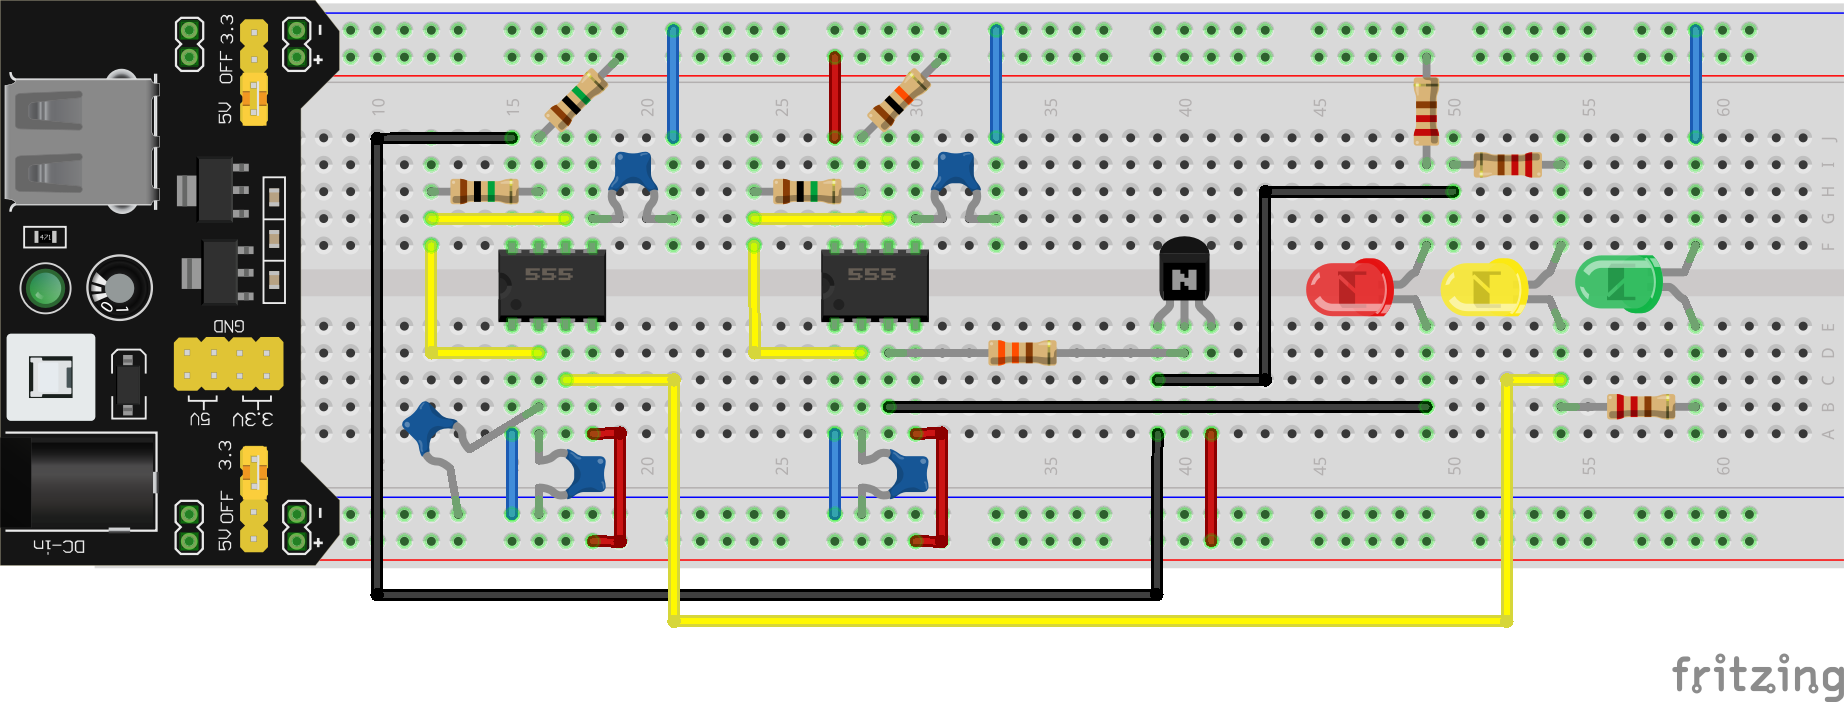
\includegraphics[width=0.8\textwidth]{lesson_circuits/L22/lesson_22.png}
    \caption{Traffic Light Breadboard Schematic}
    \label{fig:555_trlight_sch}
\end{figure}
\begin{figure}[!htp]
    \centering
    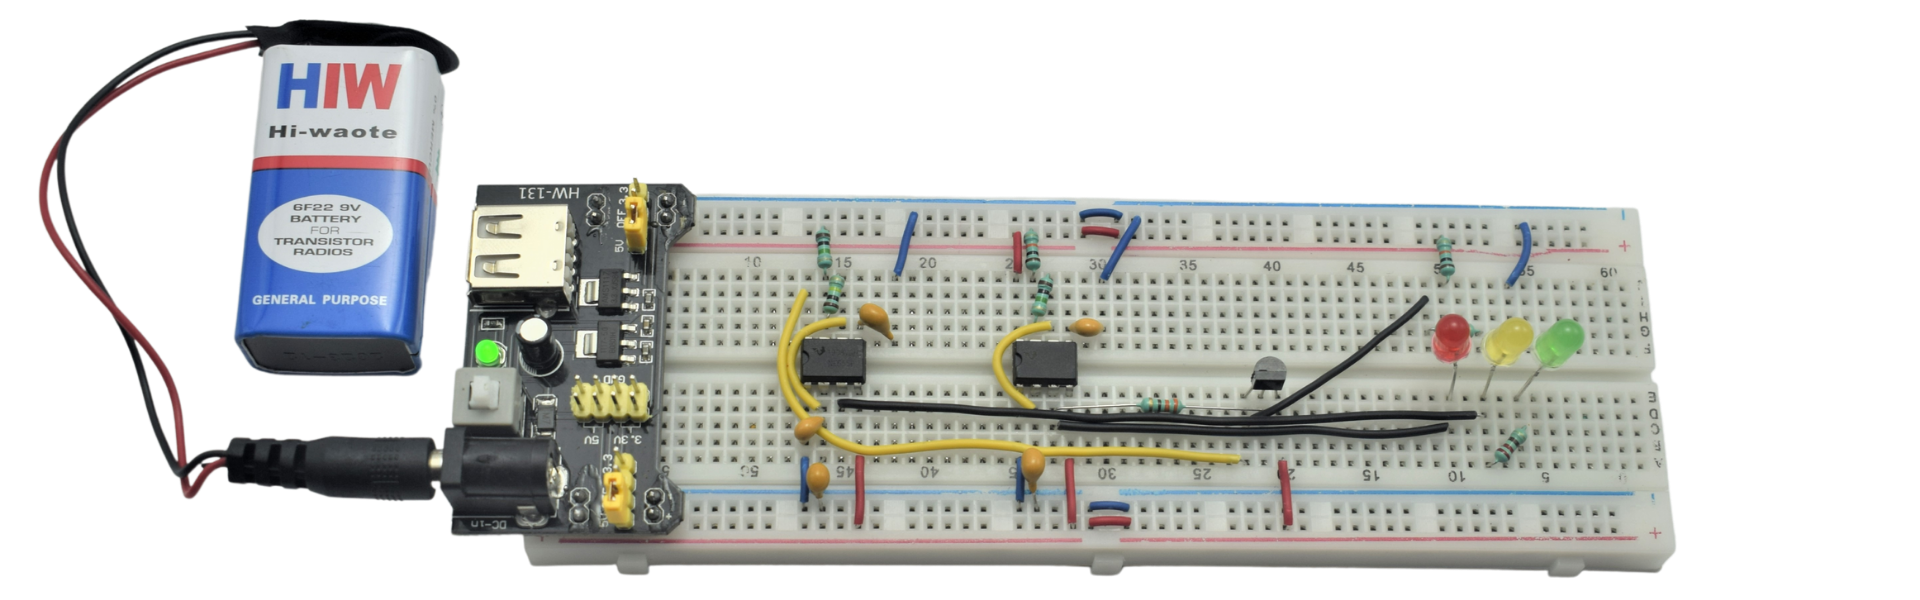
\includegraphics[width=\textwidth]{lesson_circuits/L22/L22-A.png}
    \caption{Green Light On}
    \label{fig:555_trlight_obb}
\end{figure}
\begin{figure}[!htp]
    \centering
    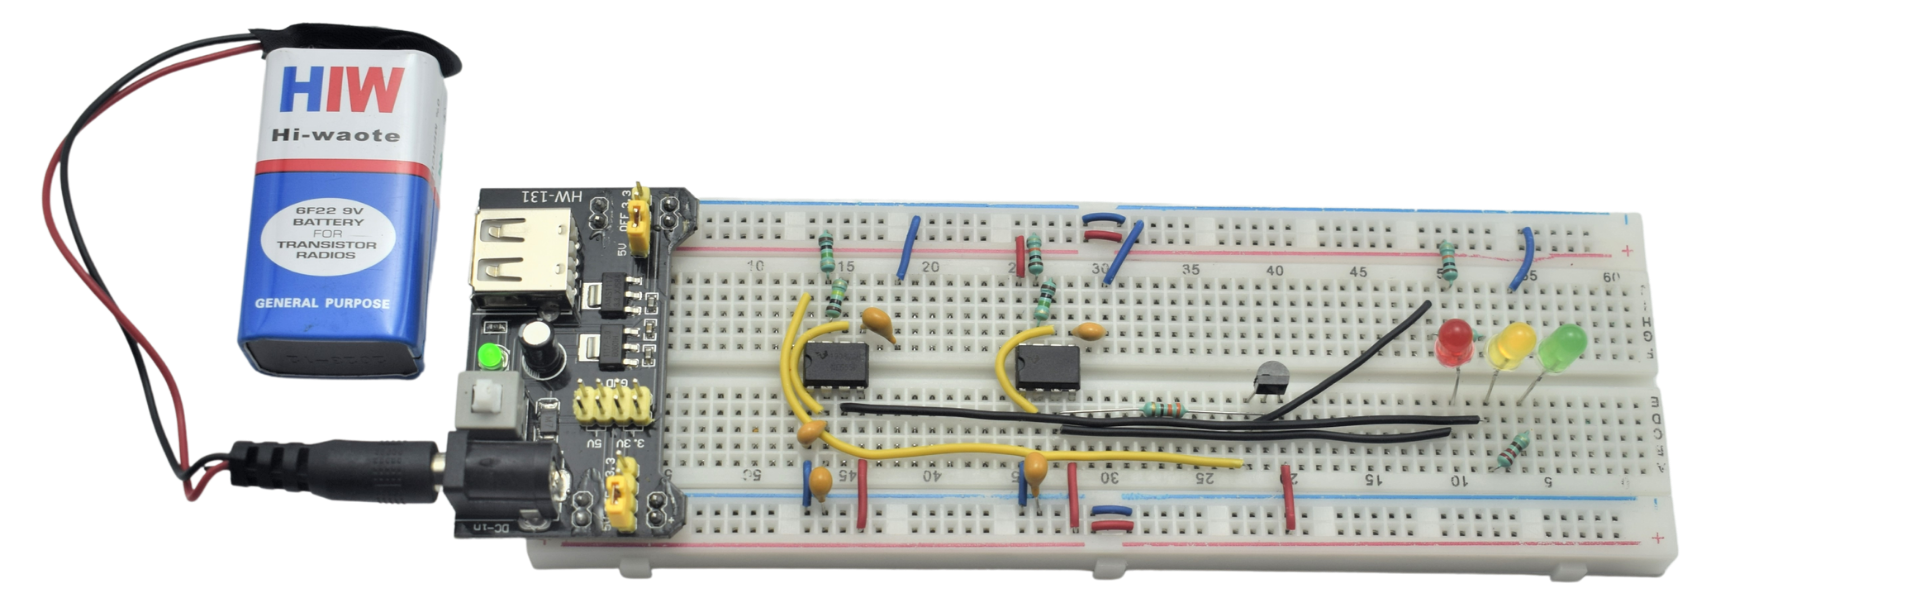
\includegraphics[width=\textwidth]{lesson_circuits/L22/L22-C.png}
    \caption{Yellow Light On}
    \label{fig:555_trlight_obb1}
\end{figure}
\begin{figure}[!htp]
    \centering
    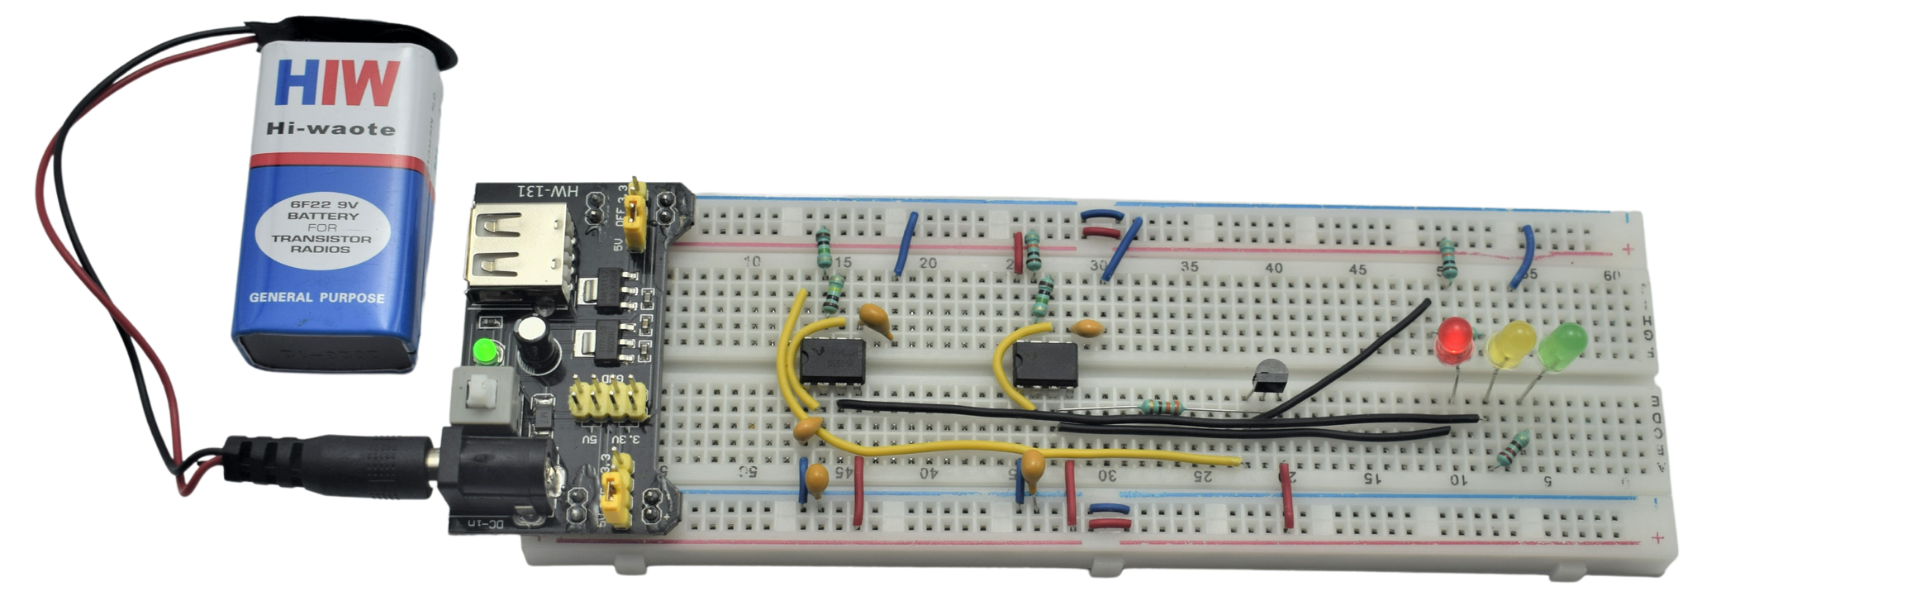
\includegraphics[width=\textwidth]{lesson_circuits/L22/L22-B.png}
    \caption{Red Light On}
    \label{fig:555_trlight_obb2}
\end{figure}
\section{Lesson 23: Doorbell}
\subsection{Objective}
In this activity we'll make a doorbell system using 555.
\subsection{Components Required}
\begin{enumerate}
    \item Breadboard Power Supply $\times$ 1
    \item 9V Battery $\times$ 1
    \item 9V Battery Connector $\times$ 1
    \item Breadboard $\times$ 1
    \item 555 IC $\times$ 2
    \item 2N2222 $\times$ 3
    \item Passive Buzzer $\times$ 1
    \item Push Button $\times$ 1
    \item \SI{1}{\kilo\ohm} $\times$ 3
    \item \SI{10}{\kilo\ohm} $\times$ 3
    \item \SI{1}{\Mohm} $\times$ 1
    \item \SI{100}{\nano\farad} $\times$ 2
    \item \SI{1}{\micro\farad} $\times$ 1
    \item Male-Male jumper wire $\times$ 23
\end{enumerate}
\subsection{Circuit}
\begin{figure}[!htp]
    \centering
    \begin{circuitikz}[scale = 1]
        \TIMER555(0,0){1}
        \draw (1 GND) to[short, -*] ++(0,-1.7) node[ground](g1){};
        \draw (1 CTRL) to[C, l=$100\si{\nano\farad}$] ++(0,-0.5)
            to[short, -*] ++(0,-1.2)node[](ctr){} |- (g1);
        \draw (1 VCC) to[short, -*] ++(0,0.5) node[vcc](v1){$V_{cc}$};
        \draw (1 RESET) |- (v1);
        \draw (1 THR) to[short, -*] ++(-0.5,0) node[](s6){};
        \draw (1 TRG) to[short, -*] ++(-1.5,0) node[](s2){};
        \draw (1 DIS) to[short, -*] ++(-0.5,0) node[](s7){};
        \draw (s7) -- ($(1 THR)-(0.5,0)$);
        \draw (s7) to[R, l=$1\si{\Mohm}$] ++(0,1.5)node[circ](a){} |- (v1);
        \draw (s6) -- ++(0,-1) to[C, l_=$1\si{\uF}$] ++(0,-2.7)node[circ](b){} |- (g1);
        \draw (s2) to[R, l=$10\si{\kohm}$] ++(0,2) |- (a);
        \draw (s2) node[npn,anchor=C](t2){$T2$};
        
        \TIMER555(8,0){2}
        %\draw (2 GND) to[short, -*] ++(0,-1.7) node[ground](2g1){};
        \draw (2 VCC) to[short, -*] ++(0,0.5) node[vcc](2v1){$V_{cc}$};
        \draw (2 RESET) to[short, -*] ++(0,0.5)node[](r2){} |- (2v1);
        \draw (2 THR) to[short, -*] ++(-0.5,0) node[](2s6){};
        \draw (2 TRG) to[short, -*] ++(-0.5,0) node[](2s2){};
        \draw (2 DIS) to[short, -*] ++(-0.5,0) node[](2s7){};
        \draw (2s7) to[R, l_=$10\si{\kohm}$] ($(2 THR)-(0.5,0)$);
        \draw (2s7) to[R, l=$10\si{\kohm}$] ++(0,1.5) |- (2v1);
        \draw (2s6) -- (2s2) to[C, l_=$100\si{\nF}$] ++(0,-1.5) 
            to[short, -*] ++(0,-1.2) node[ground](2g1){};
        \draw (2 OUT) -- ++(0.5,0) -- ++(0,-0.5)
            to[loudspeaker] ++(0,-1.5) |- (2g1);
        \draw (2 GND) -- ++(0,-0.17)node[](1ct){};
        \draw (2 CTRL) -- ++(0,-0.17)node[](1ct2){};
        \draw (1ct) node[npn, anchor=C](t1){$T1$};
        \draw (1ct2) node[npn, anchor=E,rotate=180](t3){};
        \draw (t1.E) node[circ]{};
        
        \draw (1 OUT) -| ++(1.2,-0.5) 
            to[R, l=$220\si{\ohm}$] ++ (0,-2)
            |- (t1.B);
        \draw (t2.E) |- (b);
        \draw (t2.B) -- ++(-0.5,0) to[R, l=$1\si{\kohm}$] ++(0,2.5)node[circ](c){}
            to[push button] ++(0,2) -- ++(0,0.77) to[short, -*] ++(1.35,0);
        \draw (c) -- ++(-1,0) -- ++(0,-5.5) -| (t3.B);
        \draw (t3.C) |- ++(2.5,-0.3) |- (r2);
    \end{circuitikz}
    \caption{Doorbell Circuit}
    \label{fig:555_doorbell_cir}
\end{figure}
\subsection{Circuit Explanation}
In this circuit the first 555 is in monostable mode and the second one is in astable mode. When powered on, the second 555 is 
off, as it's ground is disconnected. When the button is pressed the output of first 555 goes high, turning on the second one. 
And, the output of first 555 also controls the internal voltage of the second 555, so when the button is pressed the second 555 
sounds the buzzer in one frequency and when the button is released it sound the buzzer in different frequency till the output of 
the first 555 goes low.
\subsection{Circuit Picture}
\begin{figure}[!htp]
    \centering
    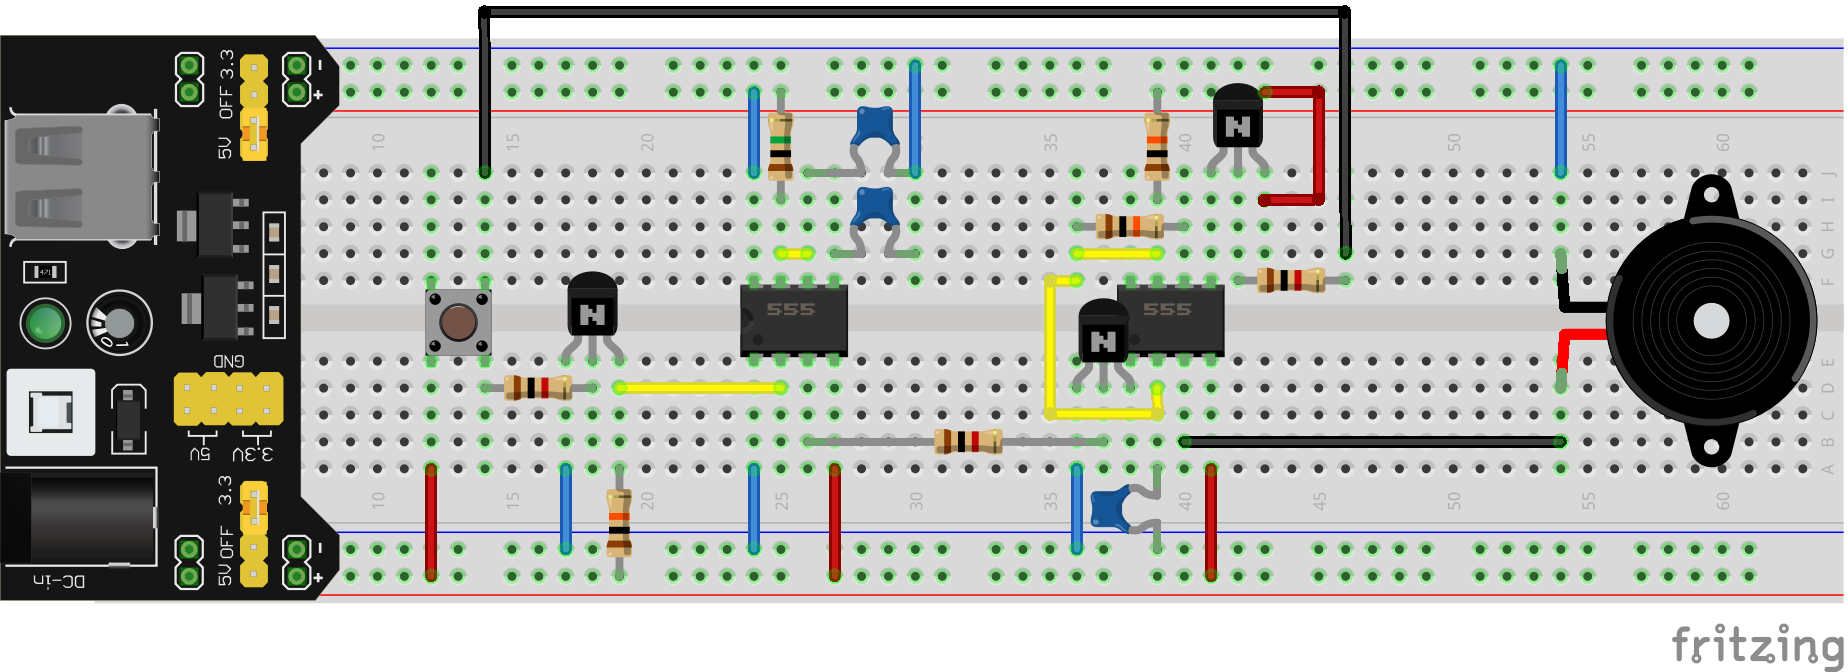
\includegraphics[width=0.8\textwidth]{lesson_circuits/L23/lesson_23.png}
    \caption{Doorbell Breadboard Schematic}
    \label{fig:555_doorbell_sch}
\end{figure}
\begin{figure}[!htp]
    \centering
    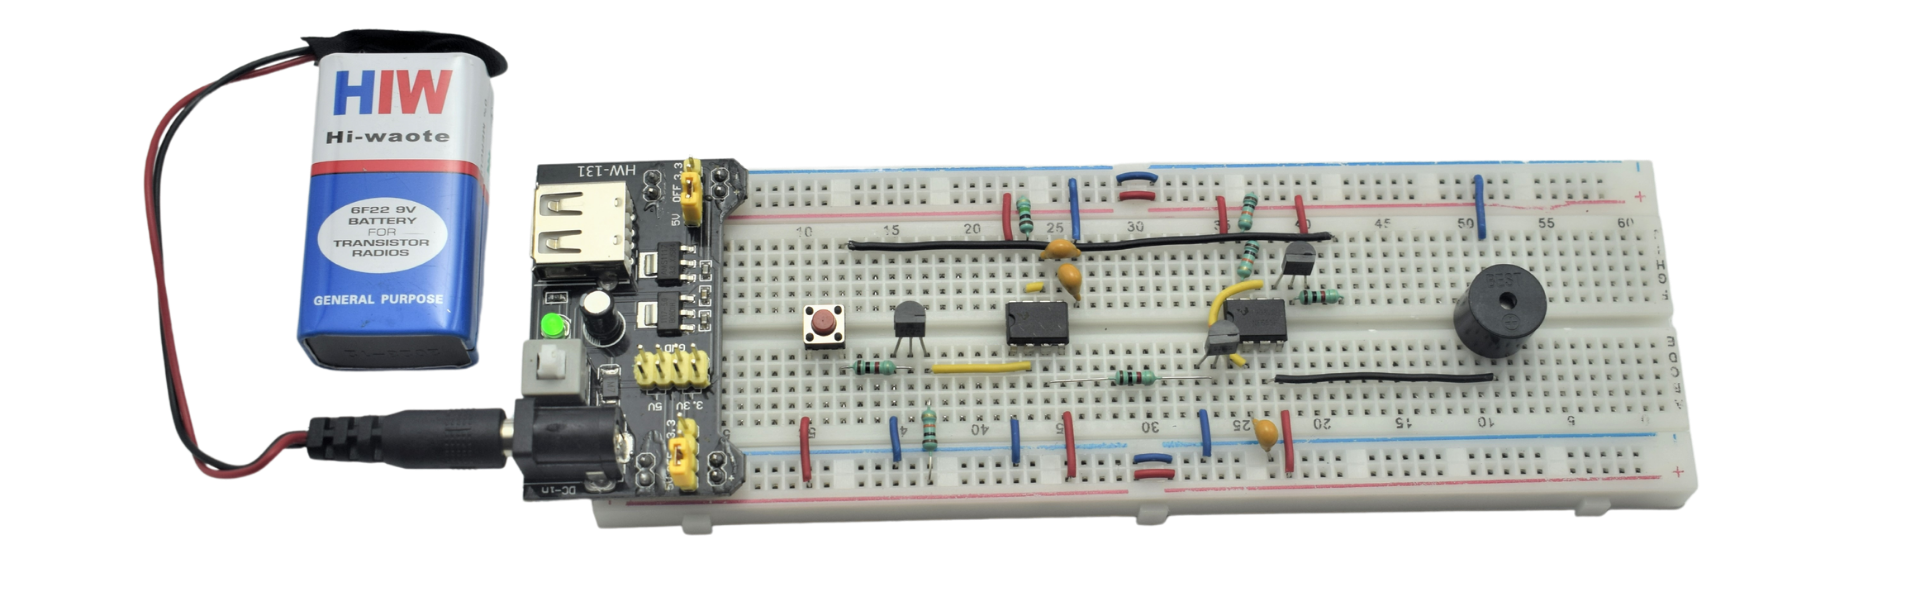
\includegraphics[width=\textwidth]{lesson_circuits/L23/L23-A.png}
    \caption{Idle: Buzzer OFF}
    \label{fig:555_doorbell_obb}
\end{figure}
\begin{figure}[!htp]
    \centering
    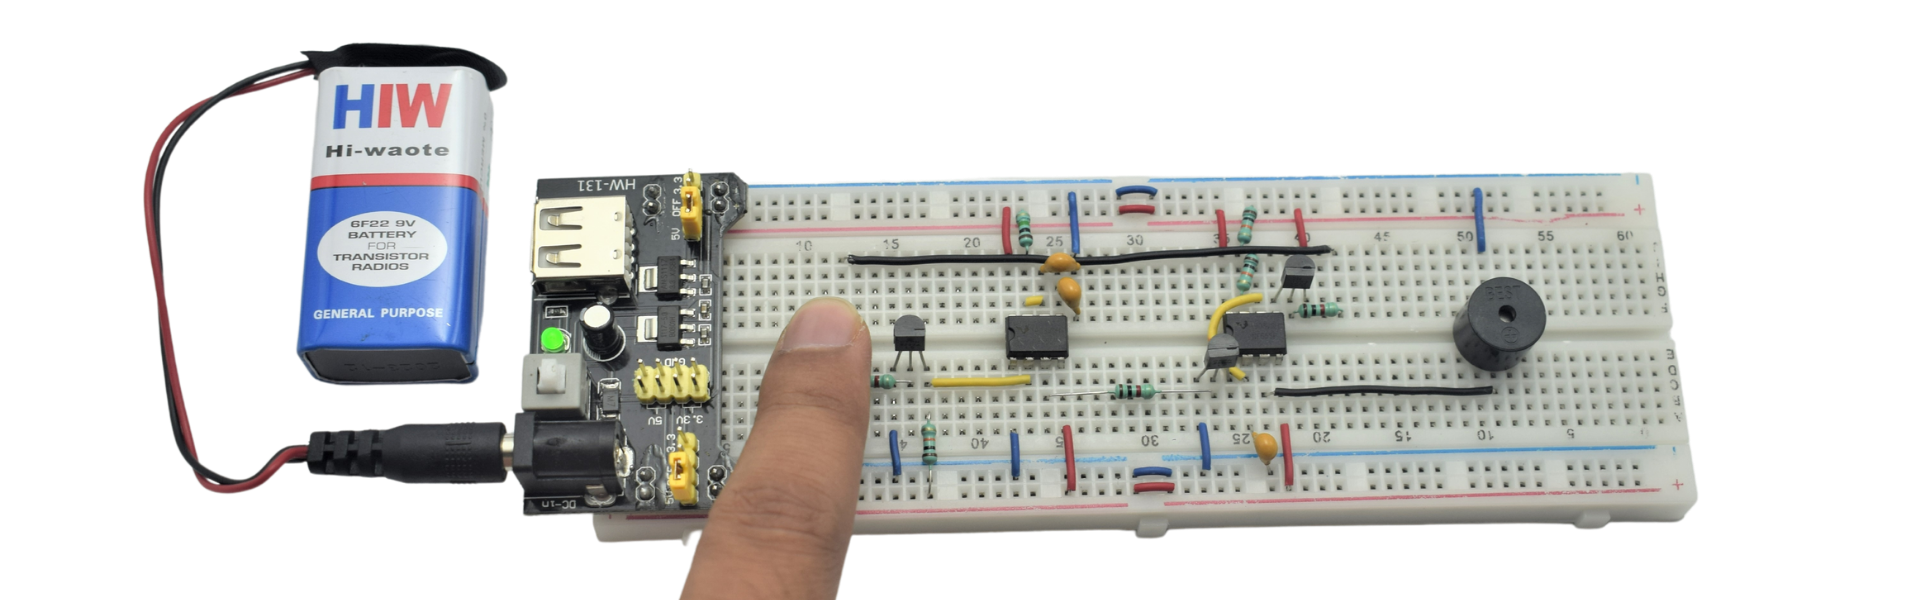
\includegraphics[width=\textwidth]{lesson_circuits/L23/L23-B.png}
    \caption{Button Pressed: Buzzer ON for sometime}
    \label{fig:555_doorbell_obb1}
\end{figure}
\section{Lesson 24: PWM Speed Controller}
\subsection{Objective}
In this activity we'll control a dc motor using 555 as PWM generator.
\subsection{Components Required}
\begin{enumerate}
    \item Breadboard Power Supply $\times$ 1
    \item 9V Battery $\times$ 1
    \item 9V Battery Connector $\times$ 1
    \item Breadboard $\times$ 1
    \item 555 IC $\times$ 1
    \item 2N2222 $\times$ 1
    \item DC Motor $\times$ 1
    \item Propeller $\times$ 1
    \item 1N4007 Diode $\times$ 2
    \item \SI{1}{\kilo\ohm} $\times$ 1
    \item \SI{2}{\kilo\ohm} $\times$ 1
    \item \SI{10}{\kilo\ohm} $\times$ 1
    \item \SI{10}{\kilo\ohm} Potentiometer $\times$ 1
    \item \SI{100}{\nano\farad} $\times$ 2
    \item \SI{10}{\micro\farad} $\times$ 1
    \item Male-Male jumper wire $\times$ 11
\end{enumerate}
\subsection{Circuit Picture}
\begin{figure}[!htp]
    \centering
    %\includegraphics[width=0.8\textwidth]{lesson_circuits/L24/lesson_24.png}
    \caption{PWM Speed Controller Breadboard Schematic}
    \label{fig:555_pwm_sch}
\end{figure}
\begin{figure}[!htp]
    \centering
    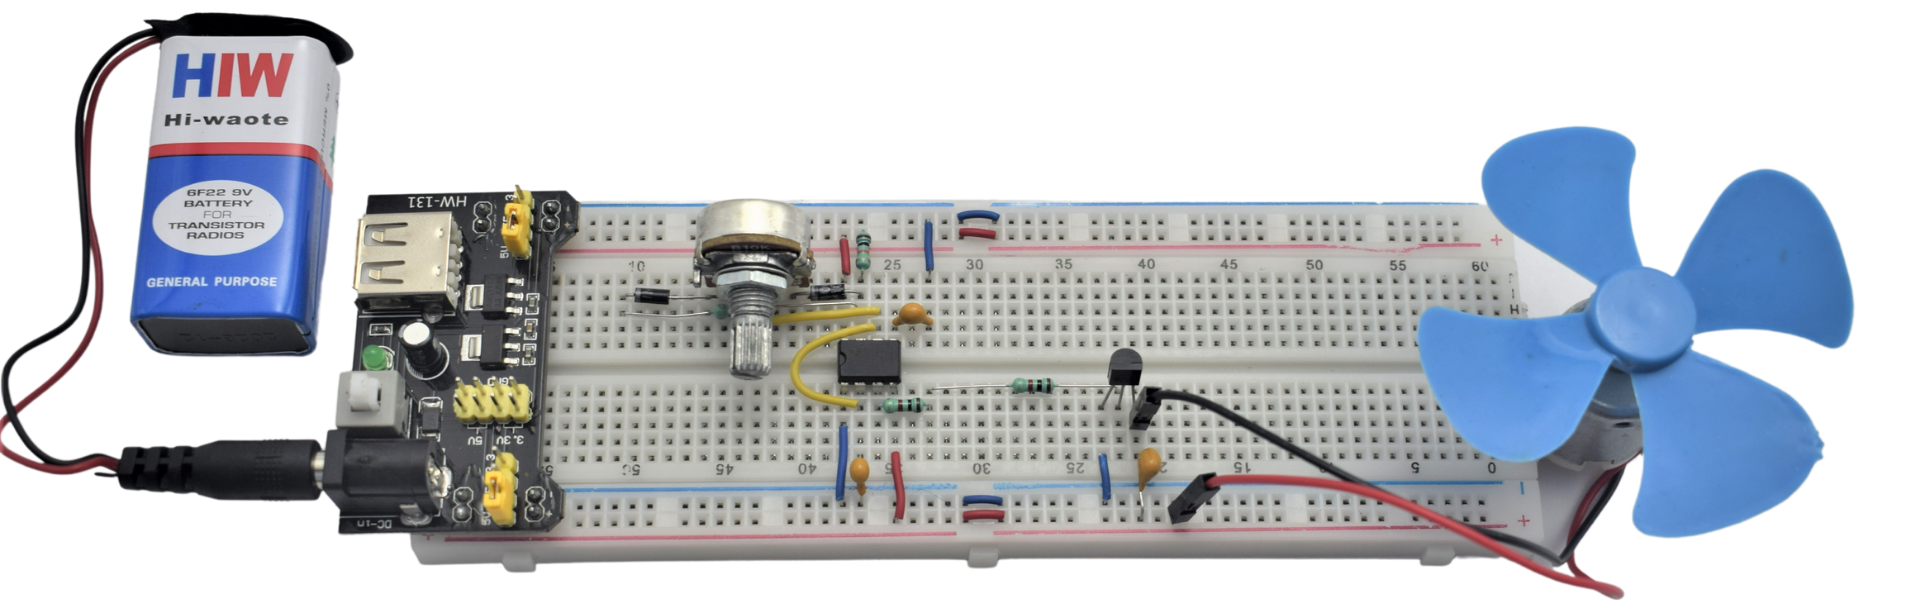
\includegraphics[width=\textwidth]{lesson_circuits/L24/L24-C.png}
    \caption{PWM 0 Duty Cycle}
    \label{fig:555_pwm_obb}
\end{figure}
\begin{figure}[!htp]
    \centering
    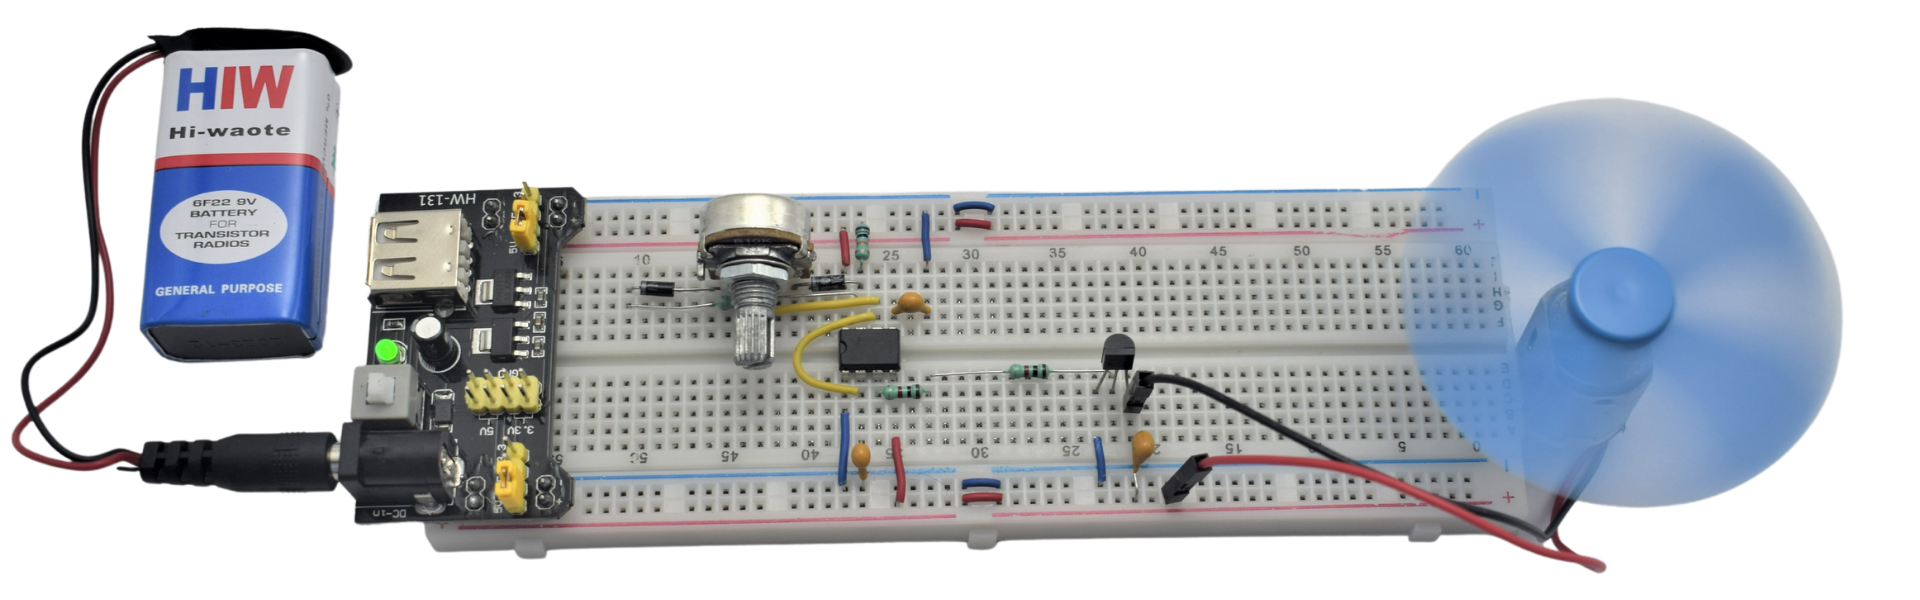
\includegraphics[width=\textwidth]{lesson_circuits/L24/L24-A.png}
    \caption{PWM half Duty Cycle}
    \label{fig:555_pwm_obb1}
\end{figure}
\begin{figure}[!htp]
    \centering
    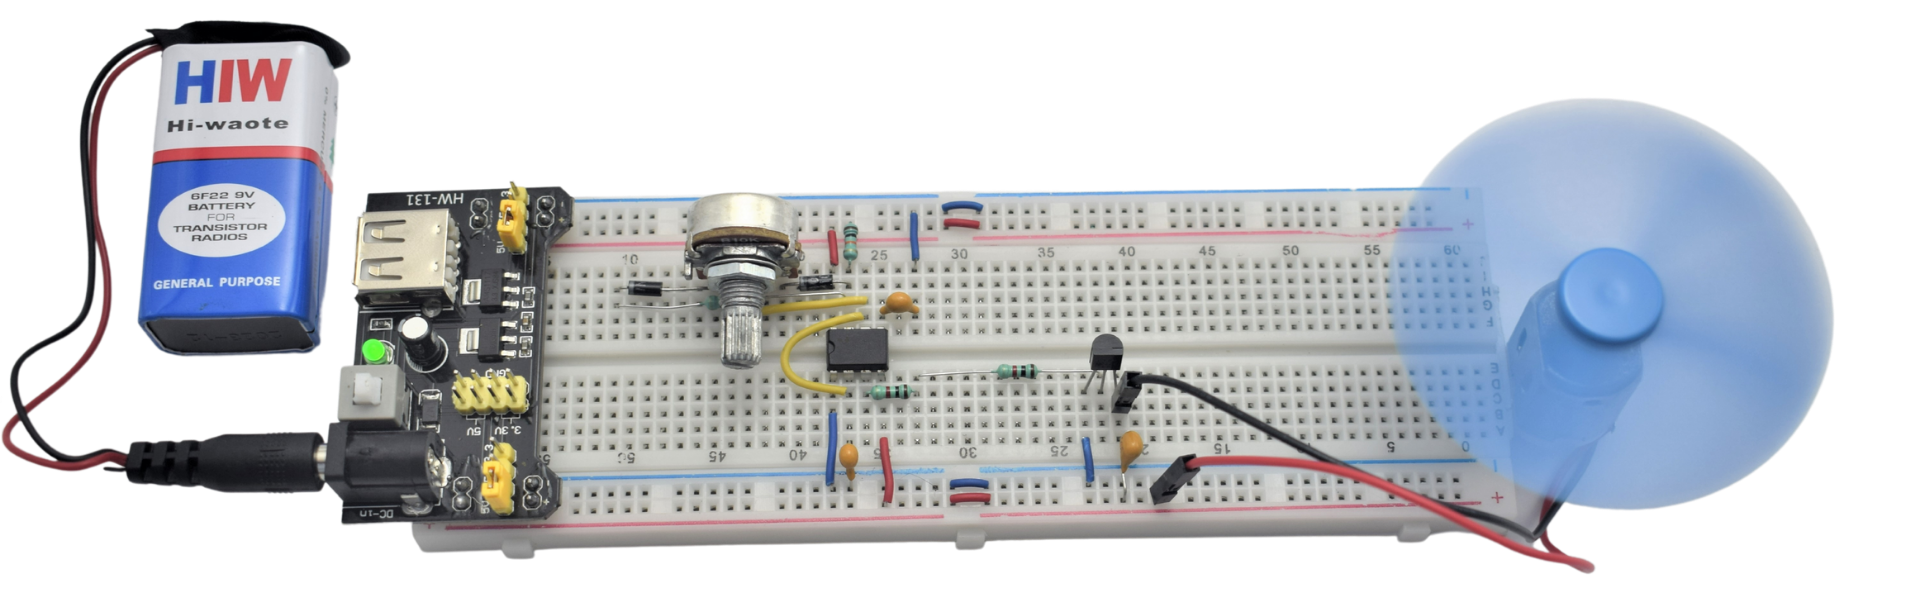
\includegraphics[width=\textwidth]{lesson_circuits/L24/L24-B.png}
    \caption{PWM full Duty Cycle}
    \label{fig:555_pwm_obb2}
\end{figure}
\section{Lesson 25: 555 RGB Flasher}
\subsection{Objective}
In this activity we'll use 3 astable 555 circuit to flash RGB LED
\subsection{Components Required}
\begin{enumerate}
    \item Breadboard Power Supply $\times$ 1
    \item 9V Battery $\times$ 1
    \item 9V Battery Connector $\times$ 1
    \item Breadboard $\times$ 1
    \item 555 IC $\times$ 3
    \item RGB LED $\times$ 1
    \item 2N2222 $\times$ 3
    \item \SI{220}{\ohm} $\times$ 3
    \item \SI{10}{\kilo\ohm} $\times$ 3
    \item \SI{100}{\kilo\ohm} $\times$ 3
    \item \SI{1}{\Mohm} $\times$ 3
    \item \SI{100}{\nano\farad} $\times$ 3
    \item \SI{2.2}{\micro\farad} $\times$ 1
    \item \SI{4.7}{\micro\farad} $\times$ 1
    \item \SI{10}{\micro\farad} $\times$ 4
    \item Male-Male jumper wire $\times$ 30
\end{enumerate}
\subsection{Circuit}
\begin{figure}[!htp]
    \centering
    \begin{circuitikz}[scale = 1]
        \TIMER555(0,8){1}
        \draw (1 GND) to[short, -*] ++(0,-0.7) node[ground](g1){};
        \draw (1 CTRL) to[C, l=$100\si{\nano\farad}$] ++(0,-0.5)
            to[short, -*] ++(0,-0.2)node[](ctr){} |- (g1);
        \draw (1 VCC) to[short, -*] ++(0,0.5) node[vcc](v1){$V_{cc}$};
        \draw (1 RESET) to[short, -*] ++(0,0.5)node[](rst){} |- (v1);
        \draw (1 THR) to[short, -*] ++(-0.5,0) node[](s6){};
        \draw (1 TRG) to[short, -*] ++(-0.5,0) node[](s2){};
        \draw (1 DIS) to[short, -*] ++(-0.5,0) node[](s7){};
        \draw (s7) to[R, l_=$10\si{\kohm}$] ($(1 THR)-(0.5,0)$);
        \draw (s7) to[R, l=$100\si{\kohm}$] ++(0,1.5) |- (v1);
        \draw (s6) -- (s2) to[C, l_=$10\si{\micro\farad}$] 
            ++(0,-1.5) |- (g1);
        \draw ($(1 OUT) + (2,0)$) node[npn](t1){};
        \draw (1 OUT) to[R,l=$100\si{\kohm}$] (t1.B);
        \draw (t1.B) to[short, *-] ++(0,-1)
                to[C, l_=$10\si{\uF}$] ++(0,-1.5) |- (ctr);
        \draw (rst) -| (t1.C);
        
        \TIMER555(0,0){2}
        \draw (2 GND) to[short, -*] ++(0,-0.7) node[ground](2g1){};
        \draw (2 CTRL) to[C, l=$100\si{\nano\farad}$] ++(0,-0.5)
            to[short, -*] ++(0,-0.2)node[](2ctr){} |- (2g1);
        \draw (2 VCC) to[short, -*] ++(0,0.5) node[vcc](2v1){$V_{cc}$};
        \draw (2 RESET) to[short, -*] ++(0,0.5)node[](2rst){} |- (2v1);
        \draw (2 THR) to[short, -*] ++(-0.5,0) node[](2s6){};
        \draw (2 TRG) to[short, -*] ++(-0.5,0) node[](2s2){};
        \draw (2 DIS) to[short, -*] ++(-0.5,0) node[](2s7){};
        \draw (2s7) to[R, l_=$10\si{\kohm}$] ($(2 THR)-(0.5,0)$);
        \draw (2s7) to[R, l=$100\si{\kohm}$] ++(0,1.5) |- (2v1);
        \draw (2s6) -- (2s2) to[C, l_=$10\si{\micro\farad}$] 
            ++(0,-1.5) |- (2g1);
        \draw ($(2 OUT) + (2,0)$) node[npn](2t1){};
        \draw (2 OUT) to[R,l=$100\si{\kohm}$] (2t1.B);
        \draw (2t1.B) to[short, *-] ++(0,-1)
                to[C, l_=$10\si{\uF}$] ++(0,-1.5) |- (2ctr);
        \draw (2rst) -| (2t1.C);
        
        \TIMER555(0,-8){3}
        \draw (3 GND) to[short, -*] ++(0,-0.7) node[ground](3g1){};
        \draw (3 CTRL) to[C, l=$100\si{\nano\farad}$] ++(0,-0.5)
            to[short, -*] ++(0,-0.2)node[](3ctr){} |- (3g1);
        \draw (3 VCC) to[short, -*] ++(0,0.5) node[vcc](3v1){$V_{cc}$};
        \draw (3 RESET) to[short, -*] ++(0,0.5)node[](3rst){} |- (3v1);
        \draw (3 THR) to[short, -*] ++(-0.5,0) node[](3s6){};
        \draw (3 TRG) to[short, -*] ++(-0.5,0) node[](3s2){};
        \draw (3 DIS) to[short, -*] ++(-0.5,0) node[](3s7){};
        \draw (3s7) to[R, l_=$10\si{\kohm}$] ($(3 THR)-(0.5,0)$);
        \draw (3s7) to[R, l=$100\si{\kohm}$] ++(0,1.5) |- (3v1);
        \draw (3s6) -- (3s2) to[C, l_=$10\si{\micro\farad}$] 
            ++(0,-1.5) |- (3g1);
        \draw ($(3 OUT) + (2,0)$) node[npn](3t1){};
        \draw (3 OUT) to[R,l=$100\si{\kohm}$] (3t1.B);
        \draw (3t1.B) to[short, *-] ++(0,-1)
                to[C, l_=$10\si{\uF}$] ++(0,-1.5) |- (3ctr);
        \draw (3rst) -| (3t1.C);
        
        \draw (8,-4) to[short, *-] ++(0,-1) node[ground]{};
        \draw (8,-4) to[full led, color=green] ++(0,1)
                to[R, l=$220\si{\ohm}$] ++(0,2)node[circ](g1){};
        \draw (8,-4) -- ++(1,0) to[full led, color=red] ++(0,1)
                to[R, l_=$220\si{\ohm}$] ++(0,2)node[circ](r1){};
        \draw (8,-4) -- ++(-1,0) to[full led, color=blue] ++(0,1)
                to[R, l=$220\si{\ohm}$] ++(0,2)node[circ](b1){};
        
        \draw (t1.E) -- ++(2,0) -| (r1);
        \draw (2t1.E) -- ++(2,0) -| (g1);
        \draw (3t1.E) -- ++(1,0) |- (b1);
        
    \end{circuitikz}
    \caption{RGB Flasher using 555 circuit}
    \label{fig:555_rgb_flash_cir}
\end{figure}
\subsection{Circuit Explanation}
In this circuit we have used 3 555 in astable configuration to flash a RGB LED.
\subsection{Circuit Picture}
\begin{figure}[!htp]
    \centering
    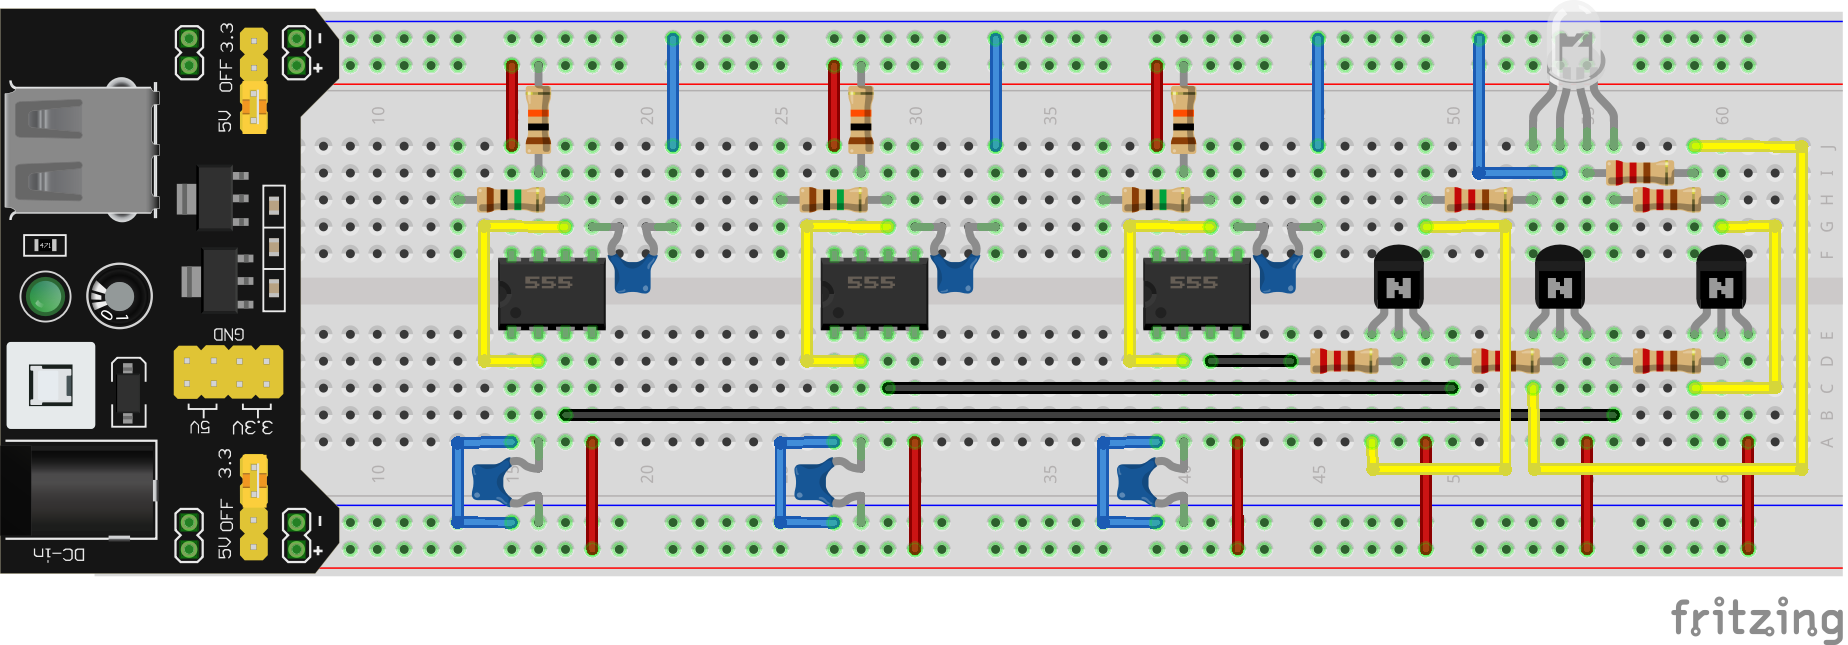
\includegraphics[width=0.8\textwidth]{lesson_circuits/L25/lesson_25.png}
    \caption{RGB LED Flasher Breadboard Schematic}
    \label{fig:555_rgb_sch}
\end{figure}
\begin{figure}[!htp]
    \centering
    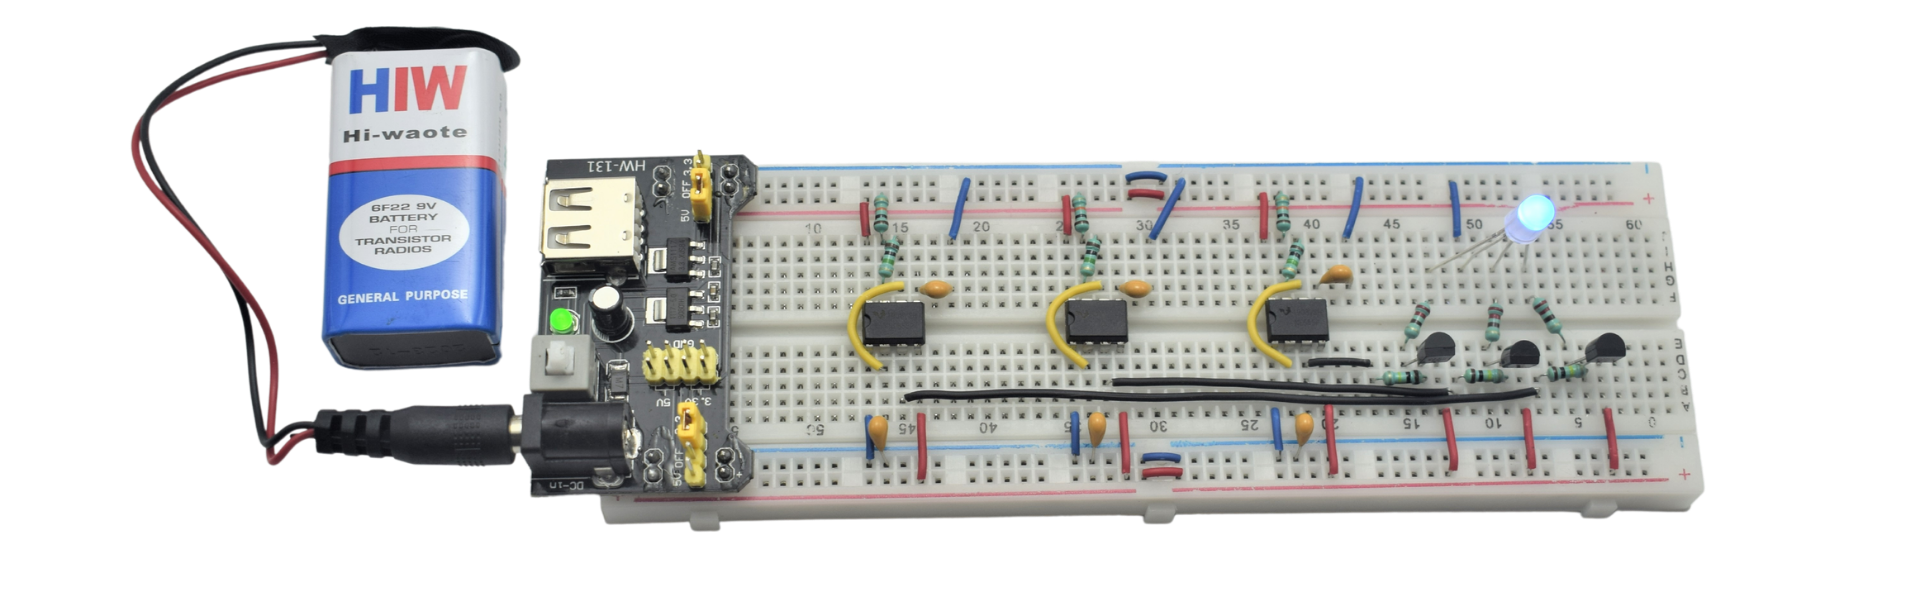
\includegraphics[width=\textwidth]{lesson_circuits/L25/L25-A.png}
    \caption{RGB Flasher}
    \label{fig:555_rgb_obb}
\end{figure}
\begin{figure}[!htp]
    \centering
    \includegraphics[width=\textwidth]{lesson_circuits/L25/L25-B.png}
    \caption{RGB Flasher}
    \label{fig:555_rgb_obb1}
\end{figure}